\documentclass[type=master]{thuthesis}
% 选项:
%   type=[bachelor|master|doctor|postdoctor], % 必选
%   secret,                                   % 可选
%   pifootnote,                               % 可选(建议打开)
%   openany|openright,                        % 可选,基本不用
%   arial,                                    % 可选,基本不用
%   arialtoc,                                 % 可选,基本不用
%   arialtitle                                % 可选,基本不用

% 所有其它可能用到的包都统一放到这里了,可以根据自己的实际添加或者删除。
\usepackage{thuthesis}

% 定义所有的图片文件在 figures 子目录下
\graphicspath{{figures/}}

% 可以在这里修改配置文件中的定义。导言区可以使用中文。
% \def\myname{薛瑞尼}

\begin{document}

%%% 封面部分
\frontmatter
\thusetup{%封面部分
  %******************************
  % 注意:
  %   1. 配置里面不要出现空行
  %   2. 不需要的配置信息可以删除
  %******************************
  %
  % 中国海洋大学研究生学位论文封面
  % 参考:中国海洋大学研究生学位论文书写格式20130307.doc
  % 为避免出现错误,下面保留[清华大学学位论文模板原有定义无需修改],
  % 请直接跳到后面[中国海洋大学学位论文模板部分请根据自己情况修改]。
  %
%%%%%%%%%%%%%%%%%%%%%%[清华大学学位论文模板原有定义无需修改]%%%%%%%%%%%%%%%%%%%%%%%
  %=====
  % 秘级
  %=====
  secretlevel={秘密},
  secretyear={10},
  %
  %=========
  % 中文信息
  %=========
  ctitle={清华大学学位论文 \LaTeX\ 模板\\使用示例文档 v\version},
  cdegree={工学硕士},
  cdepartment={计算机科学与技术系},
  cmajor={计算机科学与技术},
  cauthor={薛瑞尼},
  csupervisor={郑纬民教授},
  cassosupervisor={陈文光教授}, % 副指导老师
  ccosupervisor={某某某教授}, % 联合指导老师
  % 日期自动使用当前时间,若需指定按如下方式修改:
  % cdate={超新星纪元},
  %
  % 博士后专有部分
  cfirstdiscipline={计算机科学与技术},
  cseconddiscipline={系统结构},
  postdoctordate={2009年7月——2011年7月},
  id={编号}, % 可以留空: id={},
  udc={UDC}, % 可以留空
  catalognumber={分类号}, % 可以留空
  %
  %=========
  % 英文信息
  %=========
  etitle={An Introduction to \LaTeX{} Thesis Template of Tsinghua University v\version},
  % 这块比较复杂,需要分情况讨论:
  % 1. 学术型硕士
  %    edegree:必须为Master of Arts或Master of Science(注意大小写)
  %             “哲学、文学、历史学、法学、教育学、艺术学门类,公共管理学科
  %              填写Master of Arts,其它填写Master of Science”
  %    emajor:“获得一级学科授权的学科填写一级学科名称,其它填写二级学科名称”
  % 2. 专业型硕士
  %    edegree:“填写专业学位英文名称全称”
  %    emajor:“工程硕士填写工程领域,其它专业学位不填写此项”
  % 3. 学术型博士
  %    edegree:Doctor of Philosophy(注意大小写)
  %    emajor:“获得一级学科授权的学科填写一级学科名称,其它填写二级学科名称”
  % 4. 专业型博士
  %    edegree:“填写专业学位英文名称全称”
  %    emajor:不填写此项
  edegree={Doctor of Engineering},
  emajor={Computer Science and Technology},
  eauthor={Xue Ruini},
  esupervisor={Professor Zheng Weimin},
  eassosupervisor={Chen Wenguang},
  % 日期自动生成,若需指定按如下方式修改:
  % edate={December, 2005}
  %
  % 关键词用“英文逗号”分割
  ckeywords={\TeX, \LaTeX, CJK, 模板, 论文},
  ekeywords={\TeX, \LaTeX, CJK, template, thesis}
}

% 定义中英文摘要和关键字
\begin{cabstract}
  论文的摘要是对论文研究内容和成果的高度概括。摘要应对论文所研究的问题及其研究目
  的进行描述,对研究方法和过程进行简单介绍,对研究成果和所得结论进行概括。摘要应
  具有独立性和自明性,其内容应包含与论文全文同等量的主要信息。使读者即使不阅读全
  文,通过摘要就能了解论文的总体内容和主要成果。

  论文摘要的书写应力求精确、简明。切忌写成对论文书写内容进行提要的形式,尤其要避
  免“第 1 章……;第 2 章……;……”这种或类似的陈述方式。

  本文介绍清华大学论文模板 \thuthesis{} 的使用方法。本模板符合学校的本科、硕士、
  博士论文格式要求。

  本文的创新点主要有:
  \begin{itemize}
    \item 用例子来解释模板的使用方法;
    \item 用废话来填充无关紧要的部分;
    \item 一边学习摸索一边编写新代码。
  \end{itemize}

  关键词是为了文献标引工作、用以表示全文主要内容信息的单词或术语。关键词不超过 5
  个,每个关键词中间用分号分隔。(模板作者注:关键词分隔符不用考虑,模板会自动处
  理。英文关键词同理。)
\end{cabstract}

% 如果习惯关键字跟在摘要文字后面,可以用直接命令来设置,如下:
% \ckeywords{\TeX, \LaTeX, CJK, 模板, 论文}

\begin{eabstract}
   An abstract of a dissertation is a summary and extraction of research work
   and contributions. Included in an abstract should be description of research
   topic and research objective, brief introduction to methodology and research
   process, and summarization of conclusion and contributions of the
   research. An abstract should be characterized by independence and clarity and
   carry identical information with the dissertation. It should be such that the
   general idea and major contributions of the dissertation are conveyed without
   reading the dissertation.

   An abstract should be concise and to the point. It is a misunderstanding to
   make an abstract an outline of the dissertation and words ``the first
   chapter'', ``the second chapter'' and the like should be avoided in the
   abstract.

   Key words are terms used in a dissertation for indexing, reflecting core
   information of the dissertation. An abstract may contain a maximum of 5 key
   words, with semi-colons used in between to separate one another.
\end{eabstract}

% \ekeywords{\TeX, \LaTeX, CJK, template, thesis}
%%%%%%%%%%%%%%%%%%%%%%%%%%%%%%%%%%%%%%%%%%%%%%%%%%%%%%%%%%%%%%%%%%%%%%%%%%%%%%%%

%%%%%%%%%%%%%%%%%%[中国海洋大学学位论文模板部分请根据自己情况修改]%%%%%%%%%%%%%%%%%%%
% 中国海洋大学研究生学位论文封面
% 必须填写的内容包括(其他最好不要修改):
%   分类号、密级、UDC
%   论文中文题目、作者中文姓名
%   论文答辩时间
%   封面感谢语
%   论文英文题目
%   中文摘要、中文关键词
%   英文摘要、英文关键词
%
%%%%%[自定义]%%%%%
\newcommand{\fenleihao}{}%分类号
\newcommand{\miji}{}%密级 
                    % 绝密$\bigstar$20年 
                    % 机密$\bigstar$10年
                    % 秘密$\bigstar$5年
\newcommand{\UDC}{}%UDC
\newcommand{\oucctitle}{基于多核学习的浮游生物图像分类研究}%论文中文题目
\ctitle{基于多核学习的浮游生物图像分类研究}%必须修改因为页眉中用到
\cauthor{王如晨}%可以选择修改因为仅在 pdf 文档信息中用到
\cdegree{工学硕士}%可以选择修改因为仅在 pdf 文档信息中用到
\ckeywords{\TeX, \LaTeX, CJK, 模板, 论文}%可以选择修改因为仅在 pdf 文档信息中用到
\newcommand{\ouccauthor}{王如晨}%作者中文姓名
%\newcommand{\ouccsupervisor}{姬光荣教授}%作者导师中文姓名
%\newcommand{\ouccdegree}{博\hspace{1em}士}%作者申请学位级别
%\newcommand{\ouccmajor}{海洋信息探测与处理}%作者专业名称
%\newcommand{\ouccdateday}{\CJKdigits{\the\year}年\CJKnumber{\the\month}月\CJKnumber{\the\day}日}
%\newcommand{\ouccdate}{\CJKdigits{\the\year}年\CJKnumber{\the\month}月}
\newcommand{\oucdatedefense}{         }%论文答辩时间
%\newcommand{\oucdatedegree}{2009年6月}%学位授予时间
\newcommand{\oucgratitude}{谨以此论文献给我的导师和亲人!}%封面感谢语
\newcommand{\oucetitle}{Plankton image classification based on multiple kernel learning}%论文英文题目
%\newcommand{\ouceauthor}{Haiyong Zheng}%作者英文姓名
\newcommand{\oucthesis}{\textsc{OUCThesis}}
%%%%%默认自定义命令%%%%%
% 空下划线定义
\newcommand{\oucblankunderline}[1]{\rule[-2pt]{#1}{.7pt}}
\newcommand{\oucunderline}[2]{\underline{\hskip #1 #2 \hskip#1}}

% 论文封面第一页
%%不需要改动%%
\vspace*{5cm}
{\xiaoer\heiti\oucgratitude

\begin{flushright}
---\hspace*{-2mm}---\hspace*{-2mm}---\hspace*{-2mm}---\hspace*{-2mm}---\hspace*{-2mm}---\hspace*{-2mm}---\hspace*{-2mm}---\hspace*{-2mm}---\hspace*{-2mm}---~\ouccauthor
\end{flushright}
}

\newpage

% 论文封面第二页
%%不需要改动%%
\vspace*{1cm}
\begin{center}
  {\xiaoer\heiti\oucctitle}
\end{center}
\vspace{10.7cm}
{\normalsize\songti
\begin{flushright}
{\renewcommand{\arraystretch}{1.3}
  \begin{tabular}{r@{}l}
    学位论文答辩日期:~ & \oucunderline{2.5cm}{\oucdatedefense} \\
    指导教师签字:~ & \oucblankunderline{5cm} \\
    答辩委员会成员签字:~ & \oucblankunderline{5cm} \\
    ~ & \oucblankunderline{5cm} \\
    ~ & \oucblankunderline{5cm} \\
    ~ & \oucblankunderline{5cm} \\
    ~ & \oucblankunderline{5cm} \\
    ~ & \oucblankunderline{5cm} \\
    ~ & \oucblankunderline{5cm} \\
  \end{tabular}
}
\end{flushright}
}

\newpage

% 论文封面第三页
%%不需要改动%%
\vspace*{1cm}
\begin{center}
  {\xiaosan\heiti 独\hspace{1em}创\hspace{1em}声\hspace{1em}明}
\end{center}
\par{\normalsize\songti\parindent2em
本人声明所呈交的学位论文是本人在导师指导下进行的研究工作及取得的研究成果。据我所知,除了文中特别加以标注和致谢的地方外,论文中不包含其他人已经发表或撰写过的研究成果,也不包含未获得~\oucblankunderline{7cm}(注:如没有其他需要特别声明的,本栏可空)或其他教育机构的学位或证书使用过的材料。与我一同工作的同志对本研究所做的任何贡献均已在论文中作了明确的说明并表示谢意。
}
\vskip1.5cm
\begin{flushright}{\normalsize\songti
  学位论文作者签名:\hskip2cm 签字日期:\hskip1cm 年 \hskip0.7cm 月\hskip0.7cm 日}
\end{flushright}
\vskip.5cm
{\setlength{\unitlength}{0.1\textwidth}
  \begin{picture}(10, 0.1)
    \multiput(0,0)(0.2, 0){50}{\rule{0.15\unitlength}{.5pt}}
  \end{picture}}
\vskip1cm
\begin{center}
  {\xiaosan\heiti 学位论文版权使用授权书}
\end{center}
\par{\normalsize\songti\parindent2em
本学位论文作者完全了解学校有关保留、使用学位论文的规定,并同意以下事项:
\begin{enumerate}
\item 学校有权保留并向国家有关部门或机构送交论文的复印件和磁盘,允许论文被查阅和借阅。
\item 学校可以将学位论文的全部或部分内容编入有关数据库进行检索,可以采用影印、缩印或扫描等复制手段保存、汇编学位论文。同时授权清华大学“中国学术期刊(光盘版)电子杂志社”用于出版和编入CNKI《中国知识资源总库》,授权中国科学技术信息研究所将本学位论文收录到《中国学位论文全文数据库》。
\end{enumerate}
(保密的学位论文在解密后适用本授权书)
}
\vskip1.5cm
{\parindent0pt\normalsize\songti
学位论文作者签名:\hskip4.2cm\relax%
导师签字:\relax\hspace*{1.2cm}\\
签字日期:\hskip1cm 年\hskip0.7cm 月\hskip0.7cm 日\relax\hfill%
签字日期:\hskip1cm 年\hskip0.7cm 月\hskip0.7cm 日\relax\hspace*{1.2cm}}

\newpage

\pagestyle{plain}
\clearpage\pagenumbering{roman}

% 中文摘要
%%[需要填写:中文摘要、中文关键词]%%
\begin{center}
  {\sanhao[1.5]\heiti\oucctitle\\\vskip7pt 摘\hspace{1em}要}
\end{center}
{\normalsize\songti

  \indent
  浮游生物是海洋中生物的基本能量来源,构成了海洋食物链的基础,因此其丰富程度会影响海洋生态系统的平衡。并且,浮游生物对环境的改变较为敏感,专家们也可以利用其这一特点研究环境的变化。此外,大量有害浮游生物繁殖还会造成污染。因此,监测海洋浮游生物的分布和丰富度对海洋生态系统研究以及海洋环境保护等工作具有重要意义。

  早期对浮游生物的监测是通过人工采集浮游生物样本,并由专业人士借助显微镜等设备进行分类统计实现。这个过程不仅耗时耗力,而且专业要求高,因此导致浮游生物监测效率低下。为了解决这一问题,人们先后研制了浮游生物图像采集系统和自动识别系统,这两个系统可以高效的采集并识别大量浮游生物图像,他们的出现不仅提高浮游生物监测的效率,也降低了成本和专业需求。然而,现有浮游生物图像分类系统的泛化能力和分类性能有待提高。因此,本文以提高浮游生物图像分类系统整体性能为目标,研究并提出了基于多核学习的浮游生物图像分类系统,以提高浮游生物分类的准确率和适用范围,使其更好的应用于浮游生物监测中,主要工作如下:

  \begin{itemize}
    \item 构建不同的浮游生物数据集。为了降低所设计图像分类系统的数据集偏见,提高整个系统的泛化能力,我们搜集了不同机构和设备采集的浮游生物图像,用其构建不同的数据集进行实验,这些数据集中既包含浮游动物数据集,也包含浮游植物数据集。
    \item 研究从多角度对浮游生物的形态特征进行分析,提出结合多种有效特征的浮游生物描述方法。首先,根据浮游生物的形态,选用适合的统计方法提取几何灰度等特征;此外,将目标检测与识别领域的经典特征提取方法应用于浮游生物描述,例如局部二值模式、梯度方向直方图、内距离形状上下文等算法;然后,针对提取特征中的冗余部分,采用特征选择算法将其去除,为每个数据集保留最优的特征组合。
    \item 提出基于多核学习的浮游生物图像分类方法。对于提取的不同种类的浮游生物特征,分别为其设计适合的核函数,利用多核学习算法进行融合,从而充分发挥每种特征在分类中的积极作用。
    \item 设计对比实验,构建合理的评价体系,对提出的基于多核学习的浮游生物图像分类系统的性能进行评价。首先,根据目前应用较好的浮游生物图像分类方法设计基准实验,作为评价分类器性能的基准;然后在基准实验的基础上设计特征对比实验,对特征提取部分的性能进行评价;最后,采用本文设计的分类系统进行实验,与之前实验结果进行对比评价。
  \end{itemize}

  实验结果表明,本文提出的基于多核学习的浮游生物图像分类系统具有较好的分类性能和泛化能力,在不同浮游生物数据集上都取得了较好的分类结果。
}
\vskip12bp
{\xiaosi\heiti\noindent
关键词:\hskip1em 浮游生物,多核学习,特征提取,核函数,特征融合}

\newpage

% 英文摘要
%%[需要填写:英文摘要、英文关键词]%%
\begin{center}
  {\sanhao[1.5]\heiti\oucetitle\\\vskip7pt Abstract}
\end{center}
{\normalsize\songti

   Plankton is the main source of food for organisms in the ocean and forms the base of marine food chain. So the abundance of it will influence the ocean ecological balance. In addition, plankton is very sensitive to environment changes, thus it can be used to study the changing environment. And harmful plankton bloom pollutes the marine environment. Therefore, the study of plankton abundance and distribution is important, in order to understand environment change and protect marine ecosystems. 

   In the early days, researchers monitor the distribution and abundance of plankton with manually collecting plankton samples and classification by experts. The aforementioned process is so laborious and time consuming that hinders the plankton monitoring. To solve the problem, several imaging devices have been developed for collecting plankton images, and automatic classification system of plankton images also have been developed. The invention of imaging devices and classification system improves the efficiency of plankton monitoring. Meanwhile, the cost and specialized demand are reduced. At present, the generalization ability and classification performance wait for enhancing. This thesis studies the plankton image classification based on multiple kernel learning to improve the performance of classification system. So the system can be better used to monitor plankton. The main researches are as follows:

   \begin{itemize}
   \item Different plankton datasets are established for experiments. In order to reduce dataset bias and improve generalization ability, the plankton images gathered by different organizations and imaging devices are collected to build different datasets for experimental purposes. These datasets involve both phytoplankton dataset and zooplankton dataset.
   \item From various angles to analyze the characteristic of plankton, feasible and valid features can be combined and applied to decribe the characteristic of plankton. During the process of research, firstly, according to the characteristic of plankton, statistical methods are used to extract geometric and gray features. In addition, classical algorithms in object detection are applied to describe characteristic of plankton, such as Local Binary Pattern, Histogram of Oriented Gradients, Inner-Distance Shape Context and so on. Then, the redundant information of extracted feature is reduced by feature selection to choose the best features for each dataset.
   \item The system based on multiple kernel learning is proposed for plankton classification. In this process, predefined kernels are chose for each type of feature, and the optimal linear or non-linear combination of all kernels is learned with multiple kernel learning. So that features can give full play in classification.
   \item Contrast experiments are designed to establish system to evaluate the performance of plankton classification system. Firstly, according to the successful methods of plankton classification method at present, a baseline experiment is designed as the standard of contrast. Then, the second experiment is designed based on the baseline experiment to evaluate the property of feature extraction methods. Finally, we carry out the plankton classification system based on multiple kernel learning, and evaluate the performance of it by comparing with previous experiments.
   \end{itemize}

   Experimental results show that the plankton classification system based on multiple kernel learning has better classification performance and generalization ability. It is feasible and effective in plankton monitoring.
}
\vskip12bp
{\xiaosi\heiti\noindent 
\textbf{Keywords:\enskip plankton, multiple kernel learning, feature extraction, kernel function, feature fusion}}
%%%%%%%%%%%%%%%%%%%%%%%%%%%%%%%%%%%%%%%%%%%%%%%%%%%%%%%%%%%%%%%%%%%%%%%%%%%%%%%%
% 如果使用授权说明扫描页,将可选参数中指定为扫描得到的 PDF 文件名,例如:
% \makecover[scan-auth.pdf]
%\makecover

%% 目录
\tableofcontents

%% 符号对照表
%\begin{denotation}[3cm]
\item[HPC] 高性能计算 (High Performance Computing)
\item[cluster] 集群
\item[Itanium] 安腾
\item[SMP] 对称多处理
\item[API] 应用程序编程接口
\item[PI] 聚酰亚胺
\item[MPI] 聚酰亚胺模型化合物,N-苯基邻苯酰亚胺
\item[PBI] 聚苯并咪唑
\item[MPBI] 聚苯并咪唑模型化合物,N-苯基苯并咪唑
\item[PY] 聚吡咙
\item[PMDA-BDA]	均苯四酸二酐与联苯四胺合成的聚吡咙薄膜
\item[$\Delta G$] 活化自由能 (Activation Free Energy)
\item[$\chi$] 传输系数 (Transmission Coefficient)
\item[$E$] 能量
\item[$m$] 质量
\item[$c$] 光速
\item[$P$] 概率
\item[$T$] 时间
\item[$v$] 速度
\item[劝学] 君子曰:学不可以已。青,取之于蓝,而青于蓝;冰,水为之,而寒于水。木
  直中绳。輮以为轮,其曲中规。虽有槁暴,不复挺者,輮使之然也。故木受绳则直,金就
  砺则利,君子博学而日参省乎己,则知明而行无过矣。吾尝终日而思矣,不如须臾之所学
  也;吾尝跂而望矣,不如登高之博见也。登高而招,臂非加长也,而见者远;顺风而呼,
  声非加疾也,而闻者彰。假舆马者,非利足也,而致千里;假舟楫者,非能水也,而绝江
  河,君子生非异也,善假于物也。积土成山,风雨兴焉;积水成渊,蛟龙生焉;积善成德,
  而神明自得,圣心备焉。故不积跬步,无以至千里;不积小流,无以成江海。骐骥一跃,
  不能十步;驽马十驾,功在不舍。锲而舍之,朽木不折;锲而不舍,金石可镂。蚓无爪牙
  之利,筋骨之强,上食埃土,下饮黄泉,用心一也。蟹六跪而二螯,非蛇鳝之穴无可寄托
  者,用心躁也。—— 荀况
\end{denotation}



%%% 正文部分
\mainmatter
\chapter{绪论}
\label{cha:intro}


\section{课题研究的背景及意义}

在我们所生活的地球上,海洋是其表面上最为广阔的水域,占70\%以上。整个海洋环境以及生活在其中的动植物、微生物共同构成了海洋生态系统。在地球上,海洋生态系统为最大的生态系统,其中含有大量的浮游生物。浮游生物是海洋中其他生物的能量来源,因此为构成海洋生态系统必不可少的部分。浮游生物不仅包括浮游植物,还包括浮游动物。在海洋生态系统中,浮游植物是生成者,作为食物链的基本环节可以为其他的生物提供生活所需的能量。此外,浮游植物还会影响全球碳循环和海水中营养物质的浓度。而浮游动物以浮游植物为食,同时还是海洋食物链中高营养级动物的食物。因此,浮游动物作为海洋中生物间能力传递的桥梁,是海洋生态系统中必不可少的部分。综上,浮游动植物的丰富度及分布范围会影响整个海洋生态系统的平衡。

当浮游植物中有害的藻类大量繁殖时,会引发赤潮现象。赤潮会给海洋生态系统带来以下危害:(1)赤潮藻大量聚集会使水体缺氧,鱼类容易窒息死亡;(2)鱼类吞食有毒浮游植物会导致死亡;(3)赤潮发生后会导致水体pH值升高,造成水中生物死亡。因此,浮游植物的大量繁殖将破坏生态平衡,影响渔业的发展,甚至危害人类健康。同时,浮游动物大量繁殖也会对海洋环境造成一定的影响:(1)水域中浮游动物密度较高时会争夺海洋中其他生物的氧气;(2)浮游动物作为海洋食物链中的重要环节,它的丰富程度会影响食物链的平衡;(3)大量浮游动物聚集还会影响水下信号的传播。因此,人们越来越重视对海洋中浮游生物丰富程度的监测,这也是对海洋环境健康程度的一个评价指标。

浮游生物监测是统计在某一时间和空间范围内物种的数量以及丰富度。传统的浮游生物检测先采集样本,然后通过专业人员在显微镜下进行识别和统计,最终计算出该区域中浮游生物的丰富度。然而浮游生物体型小、数量多,人工进行采样、分类和统计不仅需要较高的专业水平,还需要消耗大量的人力、物力和时间。为了提高浮游生物监测的效率,人们研发出了浮游生物图像采集系统,可以方便的采集到水下的浮游生物图像。同时,利用图像处理和模式识别技术设计出浮游生物自动识别系统,对采集的浮游生物显微图像进行自动分类识别,可以实现对浮游生物的自动监测。这两个系统的出现大大提高了对浮游生物丰富度监测的效率,降低了成本。因此,目前人们越来越多的关注于研发性能更好的浮游生物自动分类系统,提高分类的准确率,扩大分类系统的适用范围,使其更好的应用于浮游生物丰富度的监测。



\section{国内外研究现状}
\label{sec:first}

浮游生物的自动监测主要包括浮游生物图像采集和分类识别两个部分,下面主要介绍这两部分的国内外研究现状。

\subsection{浮游生物图像采集技术}

传统的浮游生物采集通常使用网采、瓶采或泵采等方法,这些采集方法存在着一些问题:首先只能在相对较低的时间空间范围内采集样品,而且分析周期很长;其次,拖网容易扰乱浮游生物的分布结构~\cite{孙晓霞2014海洋浮游生物图像观测技术及其应用}。为了克服传统浮游生物采集方法的缺点,在过去的一段时间里浮游生物图像采集系统被广泛的研究与应用。浮游生物图像采集系统通常可以分为两类:实验室成像系统和原位图像采集系统。

实验室成像系统是指在实验室中使用的将浮游生物样本转换为数字图像的仪器设备。浮游动物图像扫描分析系统(ZooScan Integrated System)是一个比较有代表性的实验室成像系统,它由法国人Gorsky.等发明~\cite{grosjean2004enumeration},主要用于对采集到的液体样本中的浮游动物进行成像、检测、识别,该设备由ZooScan、ZooProcess和Plankton Identifier三部分组成。其中ZooScan是扫描成像部分,即图像采集部分,主要负责将采集到的浮游动物样本通过扫描的方式转换成数字图像。ZooProcess和Plankton Identifier主要对ZooScan得到的图像进行处理、测量和自动分类。目前,浮游动物图像扫描分析系统已经广泛应用于浮游动物图像采集和自动分类识别并有较高的效率和分类准确率,在国际上被广泛认可并投入商业化生产~\cite{毕永坤2011基于}。

浮游生物原位图像采集系统可以实时采集水下浮游生物原位图像,保证浮游生物的生存分布结构不被破坏。早在1992年Davis等人研制出了浮游生物视频记录器(Video Plankton Recorder, VPR)~\cite{davis1992video},这是最早的用来采集浮游生物原位图像的系统。后来随着浮游生物原位图像采集系统不断发展,先后出现了水下视频剖面仪(Underwater Video Profiler, UVP)~\cite{davis2004real}、流式细胞仪(Flow Cytometer and Microsocpe, FlowCAM)~\cite{sieracki1998imaging}、灰度图像颗粒探测系统(Shadowed Image Particle Platform and Evaluation Recorder, SIPPER)~\cite{samson2001system}、流式成像技术(Imaging FlowCytobot, IFCB)~\cite{olson2007submersible}等设备。这些设备的出现大大提高了采集浮游生物图像的效率,方便了对水下浮游生物丰富度的监测。

\subsection{浮游生物图像分类技术}
\label{chap1:sample:table} 

传统的浮游生物分类方法是生物学家根据其掌握的专业知识对采集的浮游生物样本进行人工分类。然而海洋中浮游生物种类繁多、形态各异,这使得传统人工分类方法存在以下几个问题:首先,对浮游生物进行分类时需要人员具有较高的专业水平;其次,浮游生物个体小、数量多,人工分类不仅需要大量人力,还会消耗大量时间;第三,人工分类速度较慢,难以实现对浮游生物丰富度的实时监测。因此,人们结合浮游生物图像采集系统研究出了浮游生物自动分类系统。

浮游生物自动分类系统通常采用图像处理和模式识别算法,可以对图像采集设备收集的浮游生物图像进行快速自动分类识别。其中,图像处理是为了获得图像中有用的信息,采用计算机对采集到的数字图像进行去噪、分割、增强并提取特征等操作。

早在20世纪末,硅藻图像数据库已经建立,在对该图像进行自动识别过程中人们结合了图像处理和模式识别方法。在1996年Culverhouse研发了一个对甲藻进行分类的系统,该系统提取图像中细胞的形状和表面特征进行分析,并采用了人工神经网络方法进行分类,实验结果在3种甲藻图像上的总体分类准确率可达72\%。汤晓鸥在1998年\cite{tang1998automatic}提出采用不变矩和傅里叶描述子对浮游生物视频记录器采集的浮游生物图像进行分类,该方法对含有接近2000张图像的浮游生物数据集(包括6类浮游生物)进行分类,得到的分类结果可以达到95\%。后来,在2005~\cite{zhao2005binary}和2006~\cite{tang2006binary}两年中,汤晓鸥还提出采用形状特征对二值浮游生物图像进行分类。Hu等人提出使用灰度共生矩阵描述图像中目标的灰度特征,然后采用支持向量机训练分类器。在2007年Sosik等人~\cite{sosik2007automated}结合多种特征设计了一个浮游生物分类系统,这些特征包括大小、形状、对称性、纹理等,并使用特征选择算法去掉其中的冗余部分,然后针对选择的结果采用支持向量机训练分类器,该分类系统在22类浮游生物图像上的分类准确率达到88\%。之前提到的ZooScan Integrated System~\cite{gorsky2010digital}中的Plankton Identifier是对ZooScan采集的浮游生物图像进行分类和识别的部分,该部分主要根据系统中提取的一系列描述浮游生物的形状、灰度等标量(例如面积、周长、圆形度、灰度对比度、曲率等)来进行分类,该系统在含有20类浮游动物的不平衡数据集上可以得到约78\%的分类准确率。Mosleh等~\cite{mosleh2012preliminary}采用形状和纹理特征对藻类进行描述,然后通过神经网络进行识别。在2015年Ellen等人~\cite{Quantifying2015Ellen}从不同角度对浮游生物分类方法进行分析,研究如何提高浮游生物分类的准确率。

分析国内外的研究现状可以发现,目前的浮游生物自动分类系统已经可以高效、准确的实现对采集的图像进行分类,然而也存在着一些有待改进的方面:(1)现有的分类系统中使用的特征提取方法较为单一,并不能全面的描述图像中浮游生物的形态特征;(2)部分系统在分类过程中使用多种特征描述浮游生物的形态特征,然而在融合不同特征时没有考虑每种特征的贡献比例,并不能充分发挥每种特征的积极作用;(3)由于浮游动物个体相对于浮游植物较大,并且形态相对复杂,因此人们设计的分类系统大多不能同时适用于浮游植物和浮游动物;(4)由于浮游生物种类繁多,国内外目前设计的自动分类系统大多只针对几个特定类别的浮游生物,适用范围较窄。

因此根据以上问题,我们结合多核学习设计了一个浮游生物图像分类系统,该系统从不同角度提取了浮游生物的多种特征,对形态进行全面描述;然后使用多核学习算法将所有特征融合,充分发挥每种特征在分类过程中的积极作用,提高系统的分类性能。同时,该系统具有广泛的适用范围,可以应用于不同的浮游生物数据集(既包括浮游植物也包括浮游动物),具有较好的泛化能力。


\section{课题来源}
\label{sec:complicatedtable}

国家自然科学基金项目“基于视觉注意结合生物形态特征的海洋浮游植物显微图像分析”(批准号:61301240)、国家自然科学基金项目“基于生物形态特征的中国海常见有害赤潮藻显微图像识别”(批准号:61271406)、中央高校基本科研业务费项目“海洋浮游动物原位探测与分析系统”(批准号:201562023)。


\section{论文内容和安排}
\label{sec:tableother}

本文的主要工作内容和安排如下:

第一部分为绪论,该部分主要针对浮游生物分类研究的背景意义、国内外研究现状以及课题来源进行介绍。

第二部分介绍浮游生物图像分类的预备知识,包括浮游生物的基本知识、后续实验使用的数据集、目前应用较广的浮游生物图像分类方法以及评价浮游生物分类系统性能所使用的评价方法。

第三部分根据对浮游生物形态特征的分析以及人们对浮游生物分类识别的过程,选用适合的特征提取方法,既包括简单的几何灰度特征,也包含计算机视觉领域的经典算法,例如局部二值模式、内距离形状上下文等。然后介绍特征选择算法,该方法可以去除提取特征中存在的冗余信息,保留最有效部分,从而降低特征维数,提高分类器的性能。

第四部分首先以支持向量和核函数理论为基础,介绍多核学习的基本思想,以及简单多核学习和非线性多核学习方法。然后,对设计的基于多核学习的浮游生物图像分类系统进行介绍。最后,设计一系列对系统性能进行评价的对比实验,根据对比实验的结果对基于多核学习的浮游生物图像分类系统的性能进行分析。

第五部分对本文研究的浮游生物图像分类工作进行总结,同时针对研究过程中存在的问题进行分析和展望。





\chapter{浮游生物图像分类}

研究浮游生物图像自动分类,既需要了解浮游生物领域的相关知识,也要掌握计算机视觉和机器学习领域的相关理论。本章作为介绍基于多核学习的浮游生物图像分类研究的预备知识章节,首先介绍浮游生物的基础知识,然后对后续实验使用的数据集进行说明,接下来介绍目前分类性能较好的浮游生物图像分类方法,在本章最后介绍评价分类系统性能所采用的评价方法。

\section{浮游生物基本知识介绍}

% 浮游生物介绍,分别介绍浮游植物和动物
浮游生物是指生活在水中运动能力较弱的生物体,它们是许多大型水生生物的食物,包括浮游植物和动物两大类。浮游植物是一种微小的植物,在水中以浮游状态生存,通常是指浮游藻类,包括裸藻门、黄藻门、金藻门、绿藻门、甲藻门、硅藻门、蓝藻门、隐藻门八个门类,目前已知的浮游植物约有4万种。浮游动物是生活在水中的无脊椎动物和脊索动物幼体的总称,其种类繁多,主要的门类有原生动物、浮游幼虫、甲壳纲、毛颚动物、腔肠动物、被囊动物等。

% 浮游生物个体大小
浮游生物通常较小,个体从几微米到几毫米大小不等,按照个体的大小可以将其分为以下几类:小于5微米为超微型浮游生物;5至50微米之间为微型浮游生物;50微米到1毫米之间为小型浮游生物;1至5毫米之间为中型浮游生物;5毫米到10毫米间为大型浮游生物;大于1厘米为巨型浮游生物。通常浮游植物的个体相对浮游动物较小,一般属于微型和小型浮游生物;而浮游动物体型通常较大,主要为中型、大型以及巨型浮游生物。由于大多浮游生物较小,因此必须使用显微镜进行观测。

% 浮游生物形态特征
浮游生物是按照界、门、纲、目、科、属、种的分类学原理进行分类的,从上层的“界”到下层的“种”,越往下层被归为同一个分支的浮游生物之间形态特征越相似。因此在对浮游生物进行分类时,时常会遇到形态特征十分相似的两个不同类别的浮游生物生物,这一特点增加了浮游生物分类识别的难度。例如,图~\ref{fig:changjian}中的浮游生物为长腹剑水蚤属,而图~\ref{fig:beikou}中为杯口水蚤目,这两幅图像中的浮游生物分别属于桡脚类亚纲下的剑水蚤目和杯口水蚤目,但它们的形态特征十分相似,不易区分。
\begin{figure}[h]
  \centering%
  \subcaptionbox{长腹剑水蚤属\label{fig:changjian}}%标题的长度,超过则会换行,如下一个小图。
    {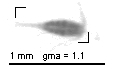
\includegraphics[height=2.5cm]{chart2/changjian}}%
  \hspace{2em}%
  \subcaptionbox{杯口水蚤目\label{fig:beikou}}
      {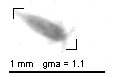
\includegraphics[height=2.5cm]{chart2/beikou}}\\
  \caption{桡脚类亚纲下的两类浮游生物图像}
  \label{fig:raojiao}
\end{figure}


\section{数据集介绍}
\label{sec:dataset}

为了设计一个泛化能力强、适用范围广的浮游生物图像分类系统,本文搜集构建了以下三个不同浮游生物数据集进行实验:一个是由伍兹霍尔海洋研究所(Woods Hole Oceanographic Institution, WHOI)使用FlowCytobot采集的浮游植物数据集;另一个是使用ZooScan系统采集的浮游动物数据集;还有Kaggle竞赛中使用的浮游生物数据集。

\subsection{WHOI采集的数据集}
\label{sec:whoidataset}

在美国的大西洋海岸上有一个综合性海洋科学研究机构——伍兹霍尔海洋研究所,其致力于对海洋中各个领域进行研究。本数据集~\cite{sosik2007automated}是由该机构研究人员使用FlowCytobot采集的2004至2005年间伍兹霍尔港附近的浮游植物图像组成,该数据集一共包括22类浮游植物图像,其例图如图~\ref{fig:whoi}所示。
\begin{figure}[H] % use float package if you want it here
  \centering
  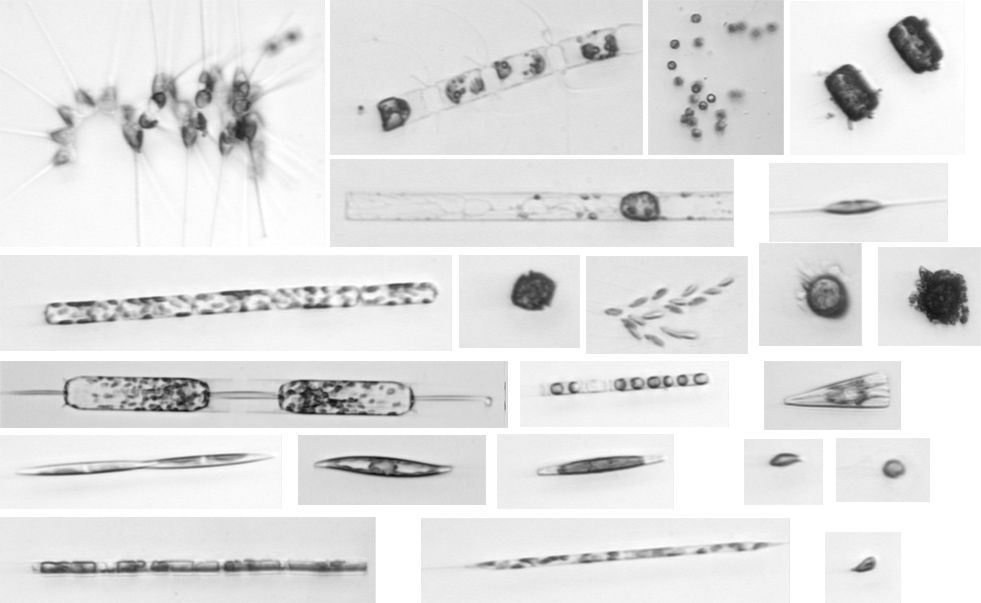
\includegraphics[height=5cm]{dataset/whoi/whoi}
  \caption{WHOI采集的数据集中每类浮游植物的例图}
  \label{fig:whoi}
\end{figure}

这22类图像中包含16类硅藻类图像:(1)星杆藻属(Asterionellopsis),(2)角毛藻属(Chaetoceros),(3)细柱藻属(Cylindrotheca),(4)指管藻属(Dactyliosolen),(5)DactFragCeratul,(6)双尾藻属(Ditylum),(7)几内亚藻属(Guinardia),(8)楔形藻属(Licmophora),(9)斜纹藻属(Pleurosigma),(10)拟菱形藻(Pseudonitzschia),(11)根管藻属(Rhizosolenia),(12)骨条藻属(Skeletonema),(13)海链藻属(Thalassiosira),(14)锥囊藻属(Dinobryon),(15)眼虫属(Euglena),(16)棕囊藻属(Phaeocystis)。除此之外还有4类由形态相似的浮游生物图像构成:(1)各种形状的纤毛虫(ciliate),(2)双鞭毛虫门(dinoflagellate),(3)鞭毛虫(nanoflagellate),(4)有翼的硅藻类(pennate diatoms)。另外还有两种海洋中的其他物质:一种是个体小于20$um$的不明物;另一种是碎石。整个数据集分为训练集和测试集,各包含3300张浮游植物图像,共6600张,其中每个类别中图像数量相等。

\subsection{ZooScan系统采集的数据集}
\label{sec:caldataset}

该数据集~\cite{gorsky2010digital}由ZooScan系统~\cite{grosjean2004enumeration}采集的浮游动物图像组成。数据集中包含20类浮游动物图像,其例图如图~\ref{fig:zooscan}所示。这20类图像中有14类为浮游动物:(1)螔螺属(Limacina),(2)翼足目(Pteropoda),(3)尖头溞属(Penilia),(4)长腹剑水蚤属(Oithona),(5)杯口水蚤目(Poecilostomatoida),(6)桡脚类亚纲(Copepoda)中的其他类生物,(7)十足目(Decapoda),(8)尾海鞘纲(Appendicularia),(9)樽海鞘纲(Thaliacae),(10)毛鄂动物门(Chaetognatha),(11)各类浮游生物的卵,(12)放射虫门(Radiolaria),(13)钟泳亚目(Calycophorae),(14)水母亚门(Medusae)。另外6类为非浮游生物:(1)气泡(bubble),(2)纤维(fiber),(3)聚集物(aggregates),(4)暗色聚集物(dark aggregates),(5)假浮游生物(pseudoplantkon),(6)采集到的聚焦不好的图像。该数据集共3771张图像,每类的图像数量各不相同,图~\ref{fig:zooscanNum}显示了数据集中每个类图像的数量,数量最少的类别有28张图像,最多的类别有427张。
\begin{figure}[H] % use float package if you want it here
  \centering
  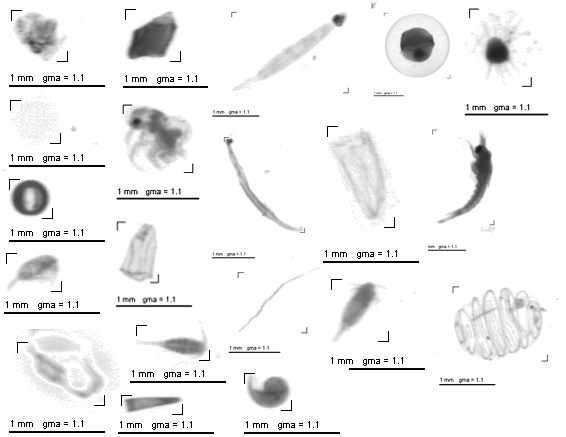
\includegraphics[height=7cm]{dataset/zooscan/zooscan}
  \caption{ZooScan系统采集的数据集中每类浮游动物的例图}
  \label{fig:zooscan}
\end{figure}
\begin{figure}[H] % use float package if you want it here
  \centering
  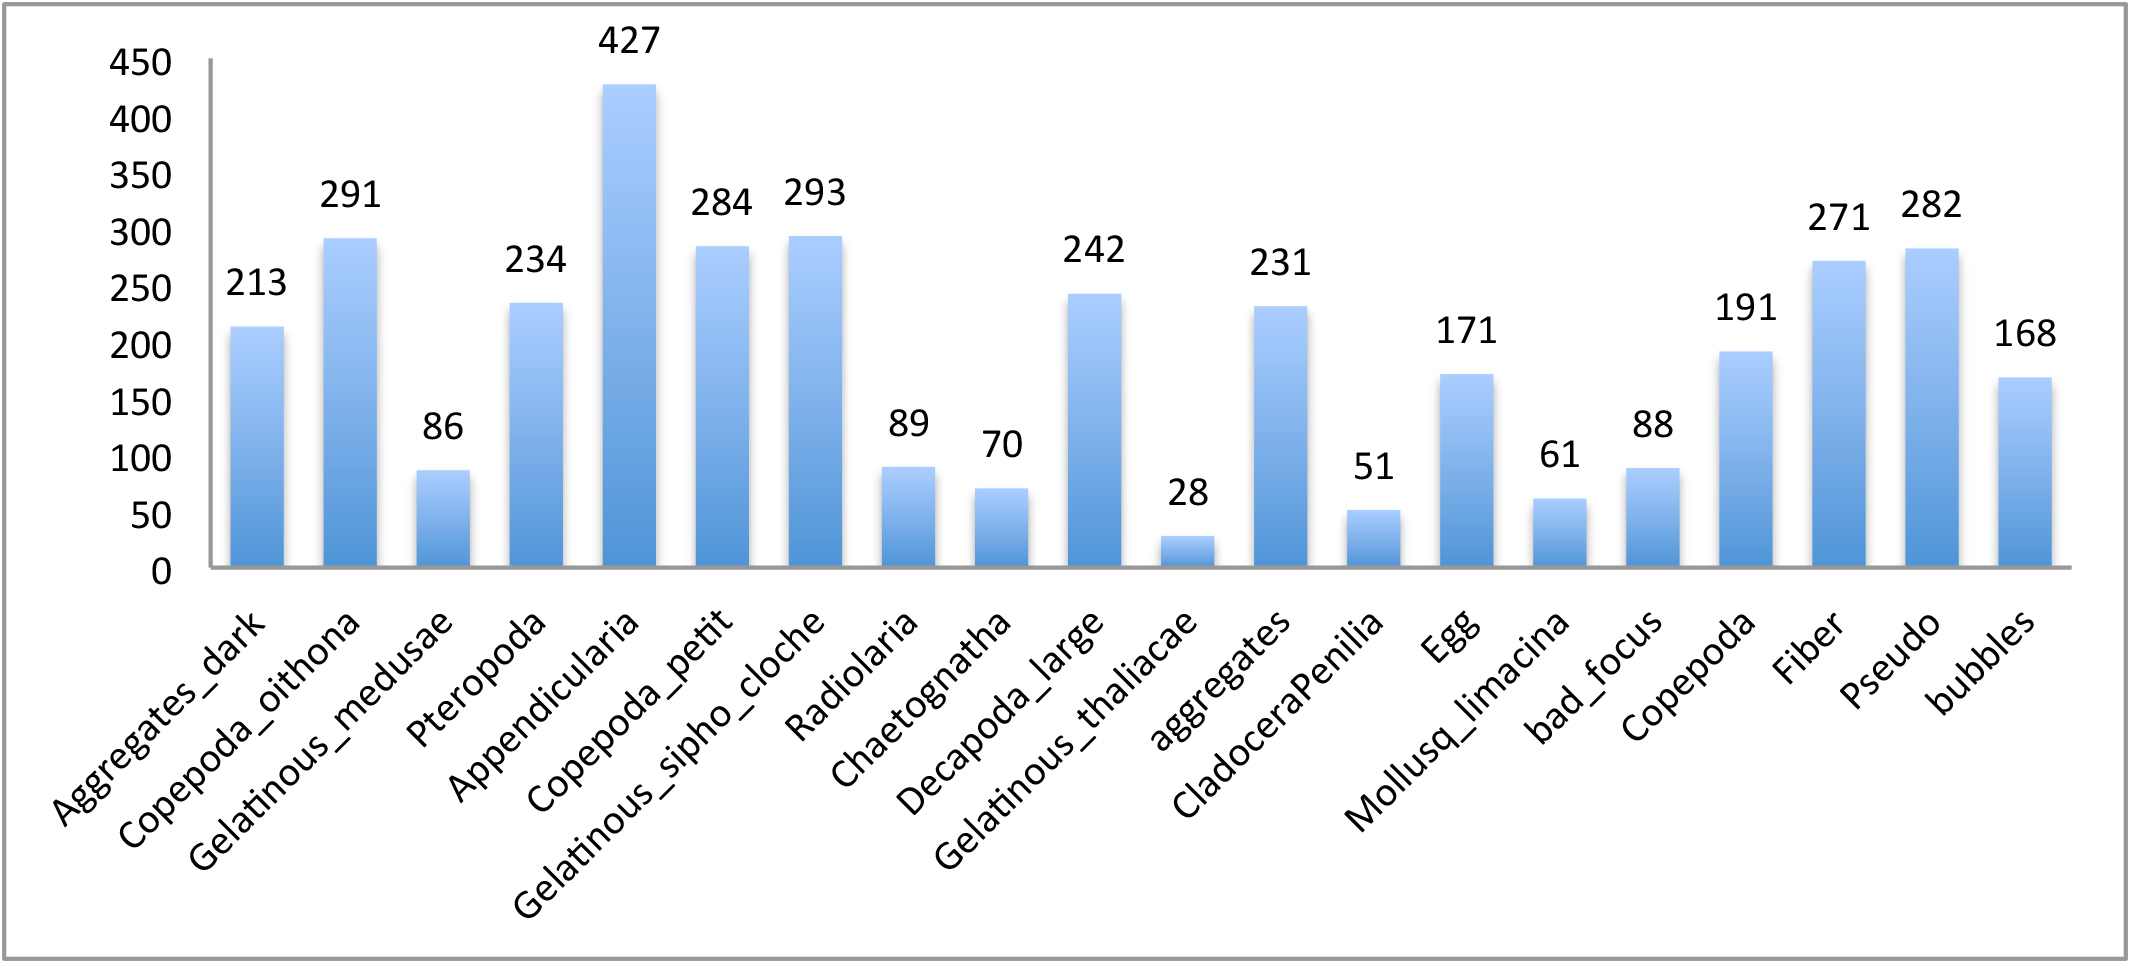
\includegraphics[height=5cm]{dataset/zooscan/zooscanNum}
  \caption{ZooScan系统采集的数据集中每类图像的数量}
  \label{fig:zooscanNum}
\end{figure}

%由于该数据集只有训练集,在用其进行实验时采用2折交叉验证的方法对分类器性能进行评价。

\subsection{Kaggle竞赛数据集}
\label{sec:kaggledataset}

Kaggle是一个数据分析的竞赛平台,研究者或企业可以将数据、问题发布在Kaggle平台上,通过竞赛的方式向大家征集解决方案。为了预测海洋健康程度,并为促进海洋健康做贡献,Kaggle竞赛平台上组织了浮游生物识别竞赛,根据浮游生物种群的丰富度衡量海洋生态系统的健康程度。Kaggle平台上的竞赛数据集由俄亥冈州立大学菲尔德海洋科学中心采集并提供,训练集共121类。本文实验中采用的数据集为该竞赛训练集的一部分,共选用38类浮游生物,例图如图~\ref{fig:kaggle}所示,其中35类为浮游生物,另外3类为非浮游生物。该数据集共28748张图像,每个类别数量各不相同,图~\ref{fig:kaggleNum}显示了每类图像的数量,数量最少的类别仅有108张图像,最多的有1979张图像。
\begin{figure}[H] % use float package if you want it here
  \centering
  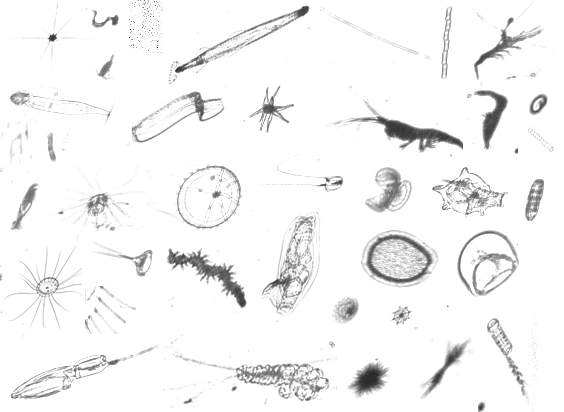
\includegraphics[height=7cm]{dataset/kaggle/kaggle}
  \caption{Kaggle竞赛数据集中每类浮游生物的例图}
  \label{fig:kaggle}
\end{figure}
\begin{figure}[H] % use float package if you want it here
  \centering
  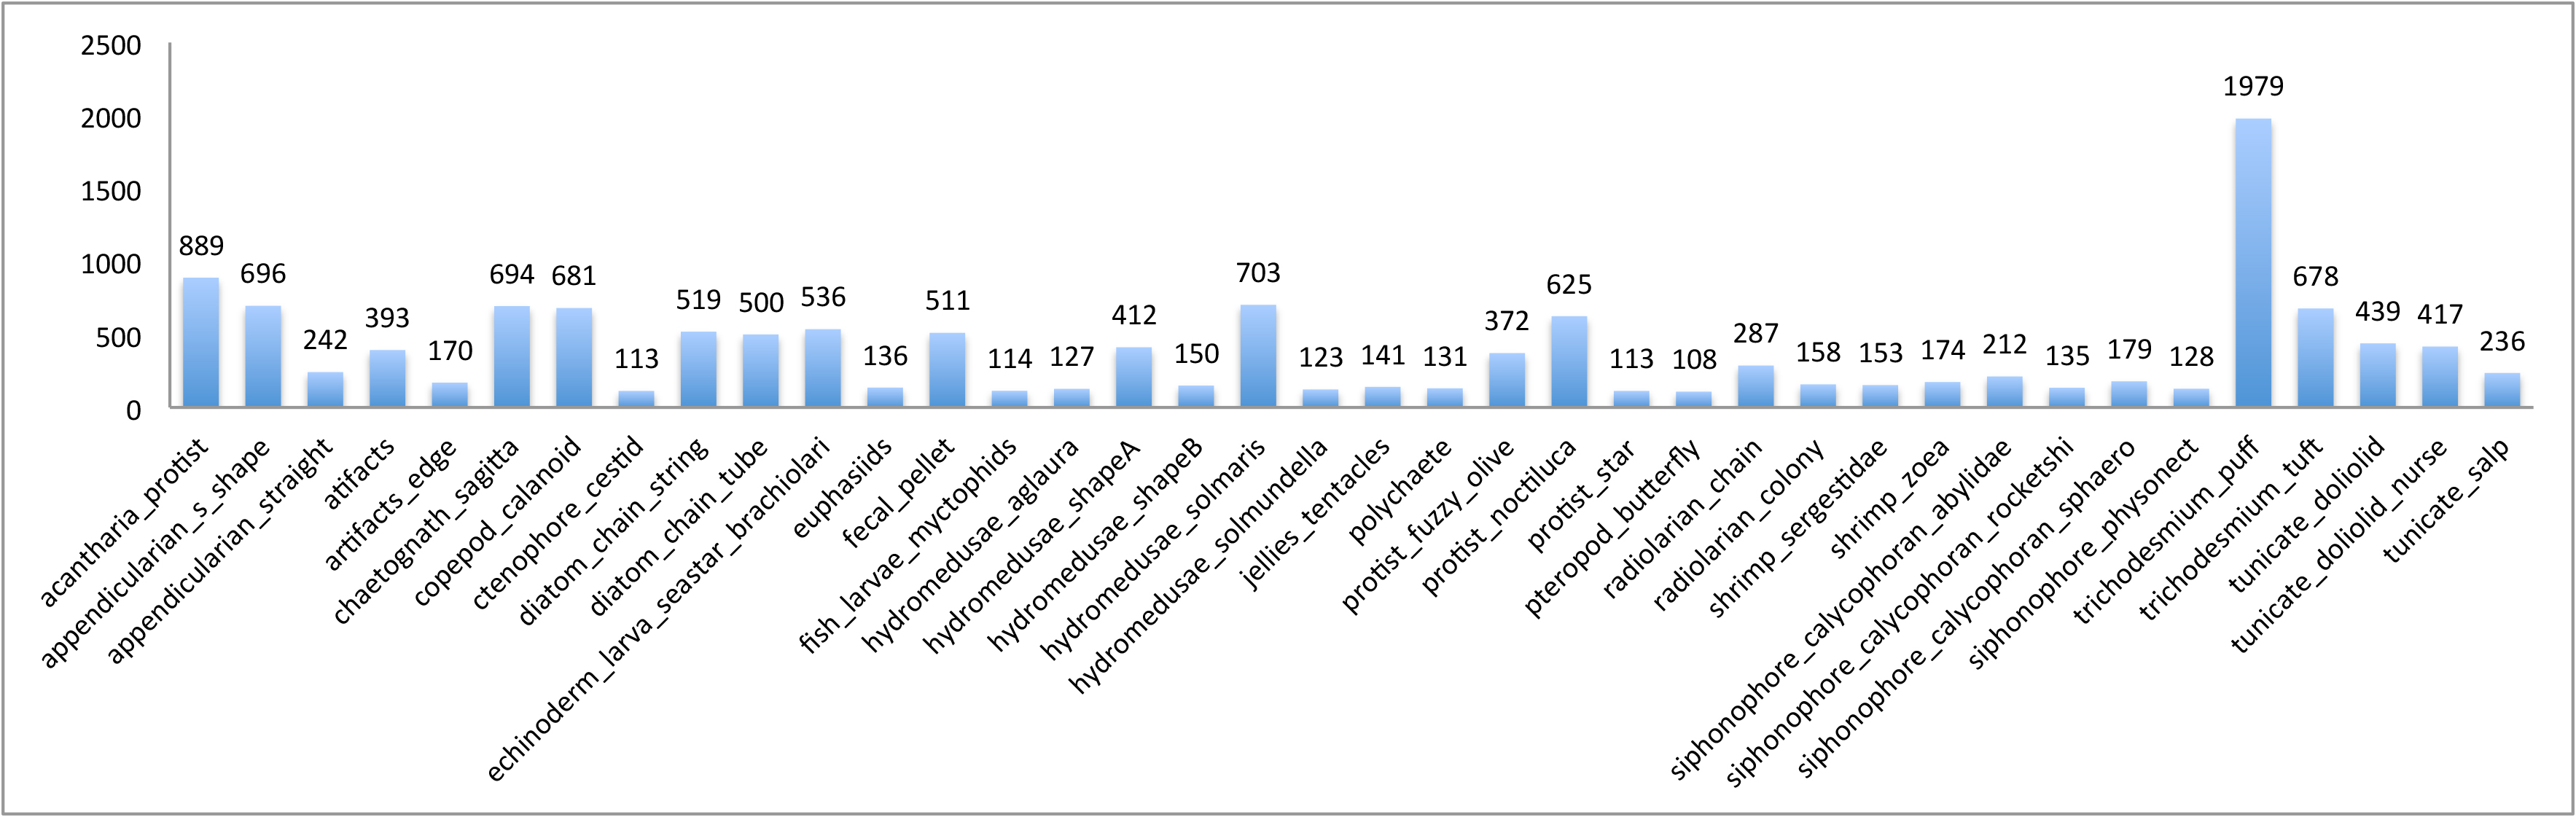
\includegraphics[height=5cm]{dataset/kaggle/kaggleNum}
  \caption{Kaggle竞赛数据集中每类图像的数量}
  \label{fig:kaggleNum}
\end{figure}


\section{浮游生物图像分类方法介绍}

目前对浮游生物图像分类的研究众多,下面分别介绍两种浮游生物图像分类系统:一个为浮游植物自动分类,由伍兹霍尔海洋研究所的Sosik等人提出;另一个是由法国国家科学院Gorsky等人研制的浮游动物图像扫描分析系统。这两个系统不仅具有较好的分类性能,而且被广泛应用于浮游生物分类,在后续实验中根据它们可以设计浮游生物分类系统性能的评价基准。

\subsection{伍兹霍尔海洋研究所浮游植物分类方法}

由于浮游生物个体小并且数量多,人工对其进行分类是不切实际的。伍兹霍尔海洋研究所的研究人员为了处理FlowCytobot采集的大量浮游植物图像,他们根据特征提取和模式识别算法提出一种浮游植物自动分类系统,该系统主要包括以下几个部分:

\begin{enumerate}
\item 图像预处理。在对图像中浮游植物形态特征进行提取时,除了需要目标的灰度纹理信息外,还需要用到目标的轮廓信息,因此要进行图像预处理,提取图像中目标生物的轮廓。在提取目标轮廓时,先采用相位一致性计算、边缘检测、数学形态学处理得到目标生物的二值图像,然后重新提取目标区域的简单边缘,从而可以获得图像中浮游生物的轮廓信息。
\item 特征提取。根据采集的原始浮游生物图像以及其对应的二值图像和轮廓边缘可以提取以下特征:简单的几何特征,例如目标的周长、长宽比、面积等;形状和对称性特征;纹理特征;不变矩;灰度共生矩阵等,共得到210个特征信息。这些特征主要通过MATLAB、DIPUM工具箱以及自定义函数生成。
\item 特征选择。由于采集的浮游生物特征中可能包含冗余或不相关的信息影响分类器的整体性能,因此采用特征选择去除冗余特征。
\item 训练分类器。特征选择后采用支持向量机来训练分类器,使用的核函数为高斯核函数(即径向基核函数),并采用10折交叉验证来确定核函数中的最优参数,该部分实验主要使用LIBSVM函数库实现。
\end{enumerate}

该分类方法在~\ref{sec:whoidataset}数据集上进行实验,使用训练集训练分类器,用获得的分类器对测试集图像进行分类,得到分类准确率可以达到88\%,其中有12个类别的分类结果超过了90\%,只有4类图像低于80\%。

\subsection{法国国家科学院浮游动物图像扫描分析系统}

浮游动物图像扫描分析系统(ZooScan Integrated System)是由法国国家科学院Villefranche海洋实验Gorsky等人发明的实验室浮游动物成像系统,该系统不仅可以完成对水下浮游动物从采集,而且能够对采集的图像进行识别~\cite{毕永坤2011基于}。与其他设备相比,ZooScan系统方便实用,并且具有较好的分类性能,目前该系统已经被广泛的商业化生产。

Zooscan系统由三部分组成,分别是Zooscan、ZooProcess和Plankton Identifier (PkID)。其中ZooScan为图像采集部分,将采集的浮游动物样本放在ZooScan仪器上,通过扫描形成数字图像。ZooProcess为软件部分,对ZooScan采集的浮游动物图像进行处理,分割提取并测量图像中的个体,可以自动得到图像中每个目标的参数,如灰度、大小、形状等参数。Plankton Identifier可以根据得到的参数对浮游生物图像进行分类。用ZooScan系统采集并识别浮游动物图像的过程如图~\ref{fig:zooscanframe}所示。
\begin{figure}[H] % use float package if you want it here
  \centering
  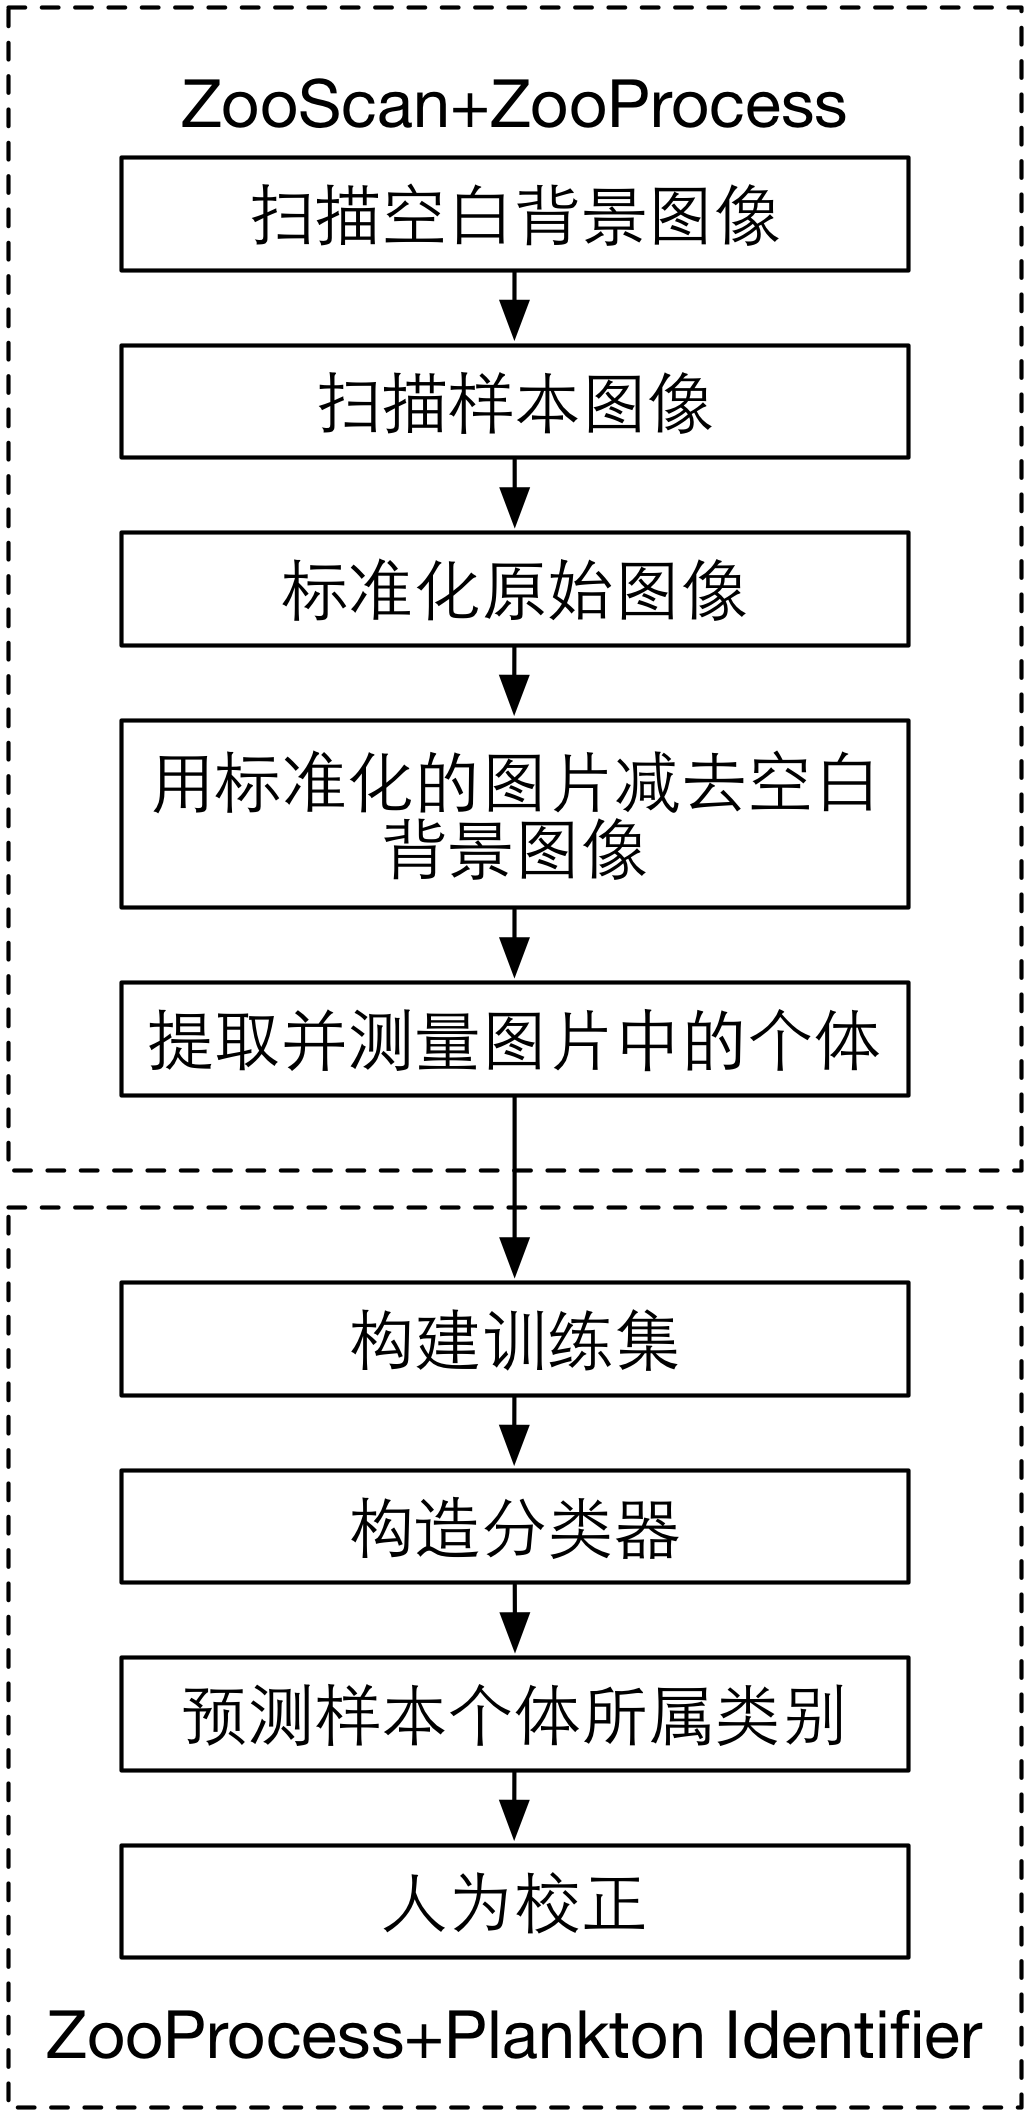
\includegraphics[height=8cm]{chart2/zooscan}
  \caption{ZooScan系统的基本流程}
  \label{fig:zooscanframe}
\end{figure}

使用ZooScan系统对采集的浮游动物进行分类时,首先用ZooProcess软件控制ZooScan扫描仪采集浮游动物图像:(1)扫描空白的背景图像;(2)扫描样本图像;(3)标准化原始图像;(4)用标准化得到的样本图像减去背景,并去除图像中的扫描框;(5)提取图像中的个体并测量每个个体的特征参数,测量得到的浮游生物特征参数共67个,大致可以分为四类:
\begin{enumerate}
\item 灰度参数,例如:
  \begin{itemize}
  \item Max,Min 物体灰度的最大、小值
  \item Mean 物体灰度的平均值
  \item IntDen 物体灰度值的总和
  \item StdDev 物体灰度值的标准差
  \end{itemize}
\item 大小参数,例如:
  \begin{itemize}
  \item Area 物体面积
  \item Perim 物体的周长
  \item Feret 物体的最大费雷特径
  \end{itemize}
\item 形状参数,例如:
  \begin{itemize}
  \item Fractal 物体的分形维数
  \item Circ 物体的圆形度
  \item Skelarea 物体骨架的像素数量
  \end{itemize}
\item 位置参数,例如:
  \begin{itemize}
  \item X,Y 物体的重心
  \item XM,YM 物体的灰度重心
  \item Height,Width 物体最小外接矩形的高和宽
  \end{itemize}
\end{enumerate}

然后,根据ZooProcess提取的特征参数,采用Plankton Identifier对采集的浮游动物图像进行分类:(1)构建训练集;(2)选用模式识别算法来训练分类器,PkID中提供的算法有K近邻、随机森林、C4.5、多层感知机、支持向量机(线性核函数、高斯核函数)等;(3)用训练得到分类器可以识别未知的浮游生物图像;(4)对预测结果进行人工校准。该分类系统在其采集的~\ref{sec:caldataset}数据集上的分类准确率可以达到78\%,分类效果最好的类别其准确率可以达到90\%以上。


\section{评价方法介绍}

评价一个分类系统性能主要从分类的准确度和可靠性两个方面进行,常用的评价方法有混淆矩阵、ROC曲线等,本文中采用的是混淆矩阵。

\subsection{混淆矩阵}

在机器学习领域,混淆矩阵(Confusion Matrix, CM)也被称为误差矩阵,是用来呈现算法性能的可视化工具,通常用于监督学习。若有n个类别,则混淆矩阵由n行n列组成,其中每一列表示每一类的预测样本数量,每一行表示每一类的实际样本数量,识别正确的样本数量为对角线,如表~\ref{tab:cm}所示。
\begin{table}[htbp]
  \centering
  \caption{混淆矩阵}
  \label{tab:cm}
  \begin{tabular}[c]{cccc}
    %\hline
    \toprule
    \multicolumn{2}{c}{\multirow{2}*{}} & \multicolumn{2}{c}{预测结果}\\
    %\cline{3-4}
    \multicolumn{2}{c}{} & 正样本 & 负样本\\
    %\hline
    \midrule
    \multirow{2}*{实际结果} & 正样本 & a & b\\
    %\cline{2-4}
     & 负样本 & c & d\\
    \bottomrule
    %\hline
  \end{tabular}
\end{table}

上表中a表示真阳性(True positives,TP),即正样本预测正确的数量;b表示正样本预测错误的样本数,即假阴性(False negatives,FN);c表示负样本被分为正样本的数目,即假阳性(False positives ,FP);d表示负样本预测正确的数量,即真阴性(True negatives ,TN)。根据这些数据可以计算出以下几个指标:
\begin{itemize}
\item 真阳性率(True positive rate,TPR),也是召回率(Recall),它表示正样本被正确识别的概率。
  \begin{eqnarray}
    TPR = \frac{a}{a+b}
  \end{eqnarray}
\item 假阳性率(False positive rate,FPR)表示负样本被误分为正样本的概率。
  \begin{eqnarray}
    FPR = \frac{c}{c+d}
  \end{eqnarray}
\item 真阴性率(True negative rate,TNR)表示负样本被正确分类的概率。
  \begin{eqnarray}
    TNR = \frac{d}{c+d}
  \end{eqnarray}
\item 假阴性率(False negative rate,FNR)表示正样本被误分为负样本的概率。
  \begin{eqnarray}
    FNR = \frac{b}{a+b}
  \end{eqnarray}
\item 错误发现率(False discovery rate,FDR)表示被预测为正样本中负样本的概率。
  \begin{eqnarray}
    FDR = \frac{c}{a+c}
  \end{eqnarray}
\item 阳性预测值(Positive predictive value,PPV),也称为命中率(Precision),表示在预测为正样本的样本中真正的正样本所占的比重。
  \begin{eqnarray}
    Precision = \frac{a}{a+c}
  \end{eqnarray}
\end{itemize}

本文实验中主要采用以下两个指标:Recall和Precision。由于Recall和Precision有时会出现矛盾情况,因此本文采用F-Measure评价分类器的性能。

%Recall越高,1-Precision越低,分类器的性能越好。

\subsection{F-Measure}

F-Measure是一种综合评价指标,也被称为F-Score,当Recall和Precision出现矛盾时,就可以采用该方法进行评价。
\begin{eqnarray}
F=\frac{(\alpha^{2}+1)P*R}{\alpha^{2}(P+R)}
\end{eqnarray}
其中$\alpha$为参数,$P$代表Precision,$R$为Recall。

当$\alpha=1$就得到F1-Measure:
\begin{eqnarray}
F1=\frac{2*PR}{P+R}
\end{eqnarray}

F1的值较高说明试验分类模型性能更好。

\subsection{交叉验证}

交叉验证(Cross Validation)是一种检验分类器性能的方法,该方法将数据集分为训练集和验证集,首先用训练集训练分类器,然后用获得的分类器对验证集进行识别,其分类结果为评价分类器性能的指标\cite{王怀亮2011交叉验证在数据建模模型选择中的应用}。在评价过程中使用交叉验证可以得到更加稳定可靠的评价结果。常用的交叉验证形式有:Hold-out验证、K折交叉验证(K-fold Cross Validation,K-CV)、留一验证(Leave-One-Out Cross Validation,LOO-CV)。
\begin{itemize}
\item Hold-out验证是将数据集划分为两集合:一个作为训练集,用其训练分类器;另一个作为验证集,用其对分类器进行测试,最终得到的分类结果可以作为该分类器的性能指标。
\item K折交叉验证就是将数据集划分为K个子集,将每一个子集分别看做验证集进行实验,与此同时另外K-1个部分作为训练集。一共要进行K次实验,训练获得K个分类模型,每个模型对验证集进行分类会得到一个准确率,这K个准确率的平均值可以作为该分类器评价指标。
\item 留一验证的基本思想为:若原数据集一共n个样本,则将每个样本单独看做验证集,另外n-1个组成训练集。与K折交叉验证类似,留意验证一共需要进行n次实验,获得n个训练模型和分类准确率,计算n个准确率的平均值可以作为分类器的评价指标。
\end{itemize}

本文对分类器性能进行评价时采用K折交叉验证。

\section{本章小结}

在介绍基于多核学习的浮游生物分类研究之前,本章先介绍了浮游生物分类的相关背景。首先介绍的是浮游生物的相关内容;然后详细介绍后续实验中所用的数据集;接下来介绍目前分类性能较好的浮游生物分类方法,在后面的实验里将根据它们设计对比实验的基准;在本章最后介绍了对分类系统性能进行评价的方法,本文使用了K折交叉验和混淆矩阵来统计得到的分类结果,从而对分类器性能进行评价。






\chapter{浮游生物特征分析}
\label{cha:phy}

在浮游生物分类过程中,特征分析是一个重要环节,得到特征的好坏会直接影响分类的最终结果。我们对浮游生物特征进行分析,根据浮游生物形态特征,从各个角度选取适合的特征提取方法进行特征描述,然后从获得的特征中选取有效的特征子集。本章主要介绍对浮游生物形态特征进行提取的方法,以及去除特征中冗余信息采用的特征选择算法。


\section{浮游生物特征提取}
\label{sec:FeatureExtraction}

人们在识别浮游生物过程中,会根据浮游生物的形状、纹理等特征对浮游生物进区分。浮游生物自动分类识别系统正是模拟人类对浮游生物分类识别的过程进行设计的,因此选择特征提取方法时可以结合人类在识别浮游生物时采用的特征。在本文中,根据浮游生物的形态特征,并结合经典计算机视觉算法对浮游生物特征进行提取,主要使用的方法有以下几种:几何灰度特征;粒子测度;纹理特征,包括变差函数、Gabor滤波器、二元梯度轮廓、局部二值模式;局部特征,包括方向梯度直方图、内距离形状上下文、尺度不变特征变换。

\subsection{几何和灰度特征}
\label{sec:graphs}

目标的几何灰度为浮游生物的基本特征,简单的几何和灰度(例如面积、周长、灰度对比度等)等统计标量可以用来表示浮游生物的形态特征。在本文的研究中,共使用43个几何和灰度特征对浮游生物进行描述,下面介绍其中部分特征。

\textbf{几何标量特征:}

\begin{enumerate}
\item 周长:为图像中包围目标的轮廓边缘上所有像素数量之和。
  \begin{eqnarray}
  L = \sum^{M}_{x=1}\sum^{N}_{y=1}n(x,y)
  \end{eqnarray}
  其中,$L$表示周长,$x,y$为像素点坐标,$n(x,y)$表示物体的边缘二值图,$M,N$为图像高和宽。
\item 面积:是指图像中目标区域内像素数量之和。
  \begin{eqnarray}
  A = \sum^{M}_{x=1}\sum^{N}_{y=1}f(x,y)
  \end{eqnarray}
  其中,$A$为面积,$f(x,y)$代表目标的二值图。
\item 体态比:表示可以包围目标的最小外接矩形的长和宽之比。
  \begin{eqnarray}
  C = \frac{W}{H}
  \end{eqnarray}
  其中,$C$为体态比,$W,H$为最小外接矩形的长宽。
\item 圆形度:表示目标区域的圆形程度。
  \begin{eqnarray}
  e = \frac{4\pi A}{L \times L}
  \end{eqnarray}
  其中,$e$表示圆形度,当$e$等于1时目标的形状为圆形,$e$越小表示目标的形状越不规律,形状与圆形差距较大。
\item 伸长率:是指可以拟合目标形状的最优椭圆的长轴和短轴之比。
  \begin{eqnarray}
  \delta = \frac{Major}{Minor}
  \end{eqnarray}
  其中,$\delta$表示伸长率,$Major$表示椭圆的长轴,$Minor$表示短轴。
\item 凸率:是指目标物体的面积与目标物体的凸壳面积之间的比值。
  \begin{eqnarray}
  C_{R} = \frac{A}{\sum^{M}_{x=1}\sum^{N}_{y=1}k(x,y)}
  \end{eqnarray}
  其中,$C_R$为凸率,$k(x,y)=\left\{ \begin{array}{ll} 1 & (x,y)\in \textrm{目标区域凸包部分}\\ 0 & (x,y)\notin \textrm{目标区域凸包部分} \end{array} \right.$。
\item 等效球直径:是指与目标物体体积相同的球的直径。
  \begin{eqnarray}
  Esc = 2 \times \sqrt{\frac{A}{\pi}}
  \end{eqnarray}
\item 最大费雷特直径:弗雷特直径是一种粒径表示方法,沿着一定方向可以测量获得的投影目标区域轮廓两边界平行线间的距离。最大弗雷特直径即目标物体轮廓边界上两平行线间距离的最大值。
\end{enumerate}

\textbf{灰度标量特征:}
\begin{enumerate}
\item 最小值:是指目标范围中全部像素点的最小灰度值。
  \begin{eqnarray}
  I_{min} = \min_{I}I(x,y)
  \end{eqnarray}
  其中,$I$表示灰度图像,$x,y$表示图像中像素点的坐标。
\item 最大值:是指目标范围中全部像素点的最大灰度值。
  \begin{eqnarray}
  I_{max}=\max_{I}I(x,y)
  \end{eqnarray}
\item 平均值:是指目标范围中全部像素点灰度值的均值。
  \begin{eqnarray}
  I_{arg} = \frac{\sum_{I}I(x,y)}{A}
  \end{eqnarray}
\item 总密度:是指目标范围中所有像素点灰度值之和。
  \begin{eqnarray}
  I_{den}=\sum_{I}I(x,y)
  \end{eqnarray}
\item 标准差:是指目标范围中灰度值的标准差。
  \begin{eqnarray}
  I_{\sigma} = \sqrt{\frac{1}{A}\sum_{I}(I(x,y)-I_{arg})^{2}}
  \end{eqnarray}
\item 对比度:表示目标区域中最亮和最暗像素区域的对比程度。
  \begin{eqnarray}
  CON = \sum^{k}_{x=1}\sum^{k}_{y=1}{G(x,y)}^2
  \end{eqnarray}
  其中,$G$表示目标图像的灰度共生矩阵,$k$表示目标图像中灰度值级数。
\item 自相关:反映目标区域中纹理的一致性。
  \begin{eqnarray}
  COR = \sum^{k}_{x=1}\sum^{k}_{y=1}\frac{xyG(x,y)-u_{x}u_{y}}{s_{x}s_{y}}
  \end{eqnarray}
  其中
  \begin{eqnarray}
  u_{x}=\sum^{k}_{x=1}\sum^{k}_{y} x G(x,y),  ~~~~  u_{y}=\sum^{k}_{x=1}\sum^{k}_{y=1} y G(x,y)
  \end{eqnarray}
  \begin{eqnarray}
  s^{2}_{x}=\sum^{k}_{x=1}\sum^{k}_{y=1}G(x,y)(x-u_{y})^{2},  ~~~~   s^{2}_{y}=\sum^{k}_{x=1}\sum^{k}_{y=1}G(x,y)(y-u_{y})^{2}
  \end{eqnarray}
\item 熵:是图像中所具有信息量的度量。
  \begin{eqnarray}
  ENT = -\sum^{k}_{x=1}\sum^{k}_{y=1}G(x,y)\log G(x,y)
  \end{eqnarray}
\end{enumerate}

除了上述几种几何和灰度特征以外,在本文还使用了不变矩、对称性等标量值来描述浮游生物的基本形态特征。

\subsection{粒子测度}

粒子测度(Granulometry)由Matheron等人在1978年提出~\cite{matheron1978randoms},可以用来计算二值图像中目标区域的大小分布情况。粒子测度的基本思想是对二值图做开运算,在开运算过程中不断增加结构元素的大小,并记录下在此过程中图像中区域内像素数量的变化。
\begin{eqnarray}
G\circ T = \cup\{T+x : T+x \subset G \}
\end{eqnarray}
\begin{eqnarray}
\psi_{\lambda}(G) = G\circ\lambda T
\end{eqnarray}

其中G为二值图,T为结构元素,$\circ$为开运算,$\lambda$为一个正数变量,表示进行开运算的次数,$\psi_{\lambda}(G)$表示经过开运算后得到的二值图像。
\begin{eqnarray}
F_{G}(\lambda) = 1-\frac{v(\psi_{\lambda}(G))}{v(G)}
\end{eqnarray}

其中$v(G)$表示得到原始图像中目标区域的像素数量,$F_{G}(\lambda)$为粒子分布,它可以描述图像中目标的区域分布特征。

在本文采用粒子测度提取浮游生物的特征,在实验中设置了两组参数,分别采用不同变换的结构元素进行开运算。第一组参数是将结构元素大小由2变到50,间隔为4,记录下图像中目标区域像素数量的变化情况。第二组参数是将结构元素大小由5变到60,间隔为5,记录图像中像素数量的变化。

\subsection{纹理特征}

\subsubsection{变差函数}

变差函数(Variogram)是Motheron在1965年提出的一种矩估计方法,可以表示区域化变量的随机性,反应了区域化变量在某个方向上某一距离范围内的相关程度。从描述纹理特征的角度来考虑,图像中浮游生物的灰度值可以看成反应图像纹理的随机性和相关程度的区域化变量~\cite{曹健渭2010基于散斑纹理变差函数的平磨表面粗糙度测量技术},因此用变差函数能够有效表示图像的纹理特性,具体形式如下:
\begin{eqnarray}
\gamma(h) = \frac{1}{2N(h)}\sum^{N(h)}_{i=1}[Z(x)-Z(x+h)]^{2}
\end{eqnarray}

其中$h$是两个像素之间沿着某一方向的距离,$N(h)$是指在一定的区域内像素间距离为h的对数,$Z(x)$和$Z(x+h)$为点$x$和$x+h$的灰度值。用变差函数描述纹理特征时,选用一定的窗口、步长和方向计算函数值,然后取平均值赋给窗口中心点,得到差变函数纹理图。

\subsubsection{Gabor滤波器}
\label{sec:multifig}

Gabor滤波器是一种基于信号处理的纹理分析方法,其实质是一种加了高斯窗口的傅里叶变换,通过窗口的变化可以提取图像不同尺度和不同位置上的纹理信息。Gabor变换符合人和动物的视觉机理,具有良好的方向选择性和空间局部性~\cite{高梓瑞2012gabor},可以精确的描述局部纹理特性,因此该方法被广泛的用来提取纹理特征。本文中使用二维Gabor滤波器来描述浮游生物的纹理特征。

二维Gabor滤波器的冲击响应为~\cite{王铌2006海洋浮游生物数字图像处理方法}:
\begin{eqnarray}
h(x,y) = \frac{1}{2\pi \sigma^{2}} e^{-\frac{x^{2}+y^{2}}{2\sigma^{2}}+2\pi jF(x\cos\theta+y\sin\theta)}
\end{eqnarray}
其中$\theta$为方向,$F$为中心频率,这两个参数决定着Gabor滤波器的位置,即改变这两个参数可以得到不同滤波通道。Gabor滤波器的本质就是与原图像进行卷积,即
\begin{eqnarray}
Q(x,y)=I(x,y)*h(x,y)
\end{eqnarray}
其中$I(x,y)$为原图像,$Q(x,y)$为Gabor滤波的结果。采用不同参数卷积后会得到不同的输出图像,每幅输出图像的均值和标准差可以表示该图像的纹理特性,所有图像的值可以组成一个特征向量来描述原始图像的纹理特征。
\begin{eqnarray}
mean = \frac{\sum^{n-1}_{x=0}\sum^{m-1}_{y=0}Q(x,y)}{m \times n}
\end{eqnarray}
\begin{eqnarray}
std=\sqrt{\frac{\sum^{n-1}_{x=0}\sum^{m-1}_{y=0}[Q(x,y)-mean]^{2}}{m \times n}}
\end{eqnarray}
其中$m, n$表示图像的长和宽,mean和std分别为卷积后图像的均值和标准差。若在实验中参数选用a个方向,b个中心频率,那么一共会得到$a \times b$个不同的Gabor滤波器,从而获得$a \times b$张图像。然后分别计算每张滤波后得到图像的均值和标准差,将获得$a \times b \times 2$个值组成一个特征向量,该向量可以有效的描述目标图像的纹理特征。在本文实验中,我们为Gabor滤波器选定了不同的参数,包括6个频率、8个方向,如图~\ref{fig:gabor}。用Gabor滤波器提取特征时,每幅图像会获得一个96($6 \times 8 \times 2$)维的特征向量。
\begin{figure}[H] % use float package if you want it here
  \centering
  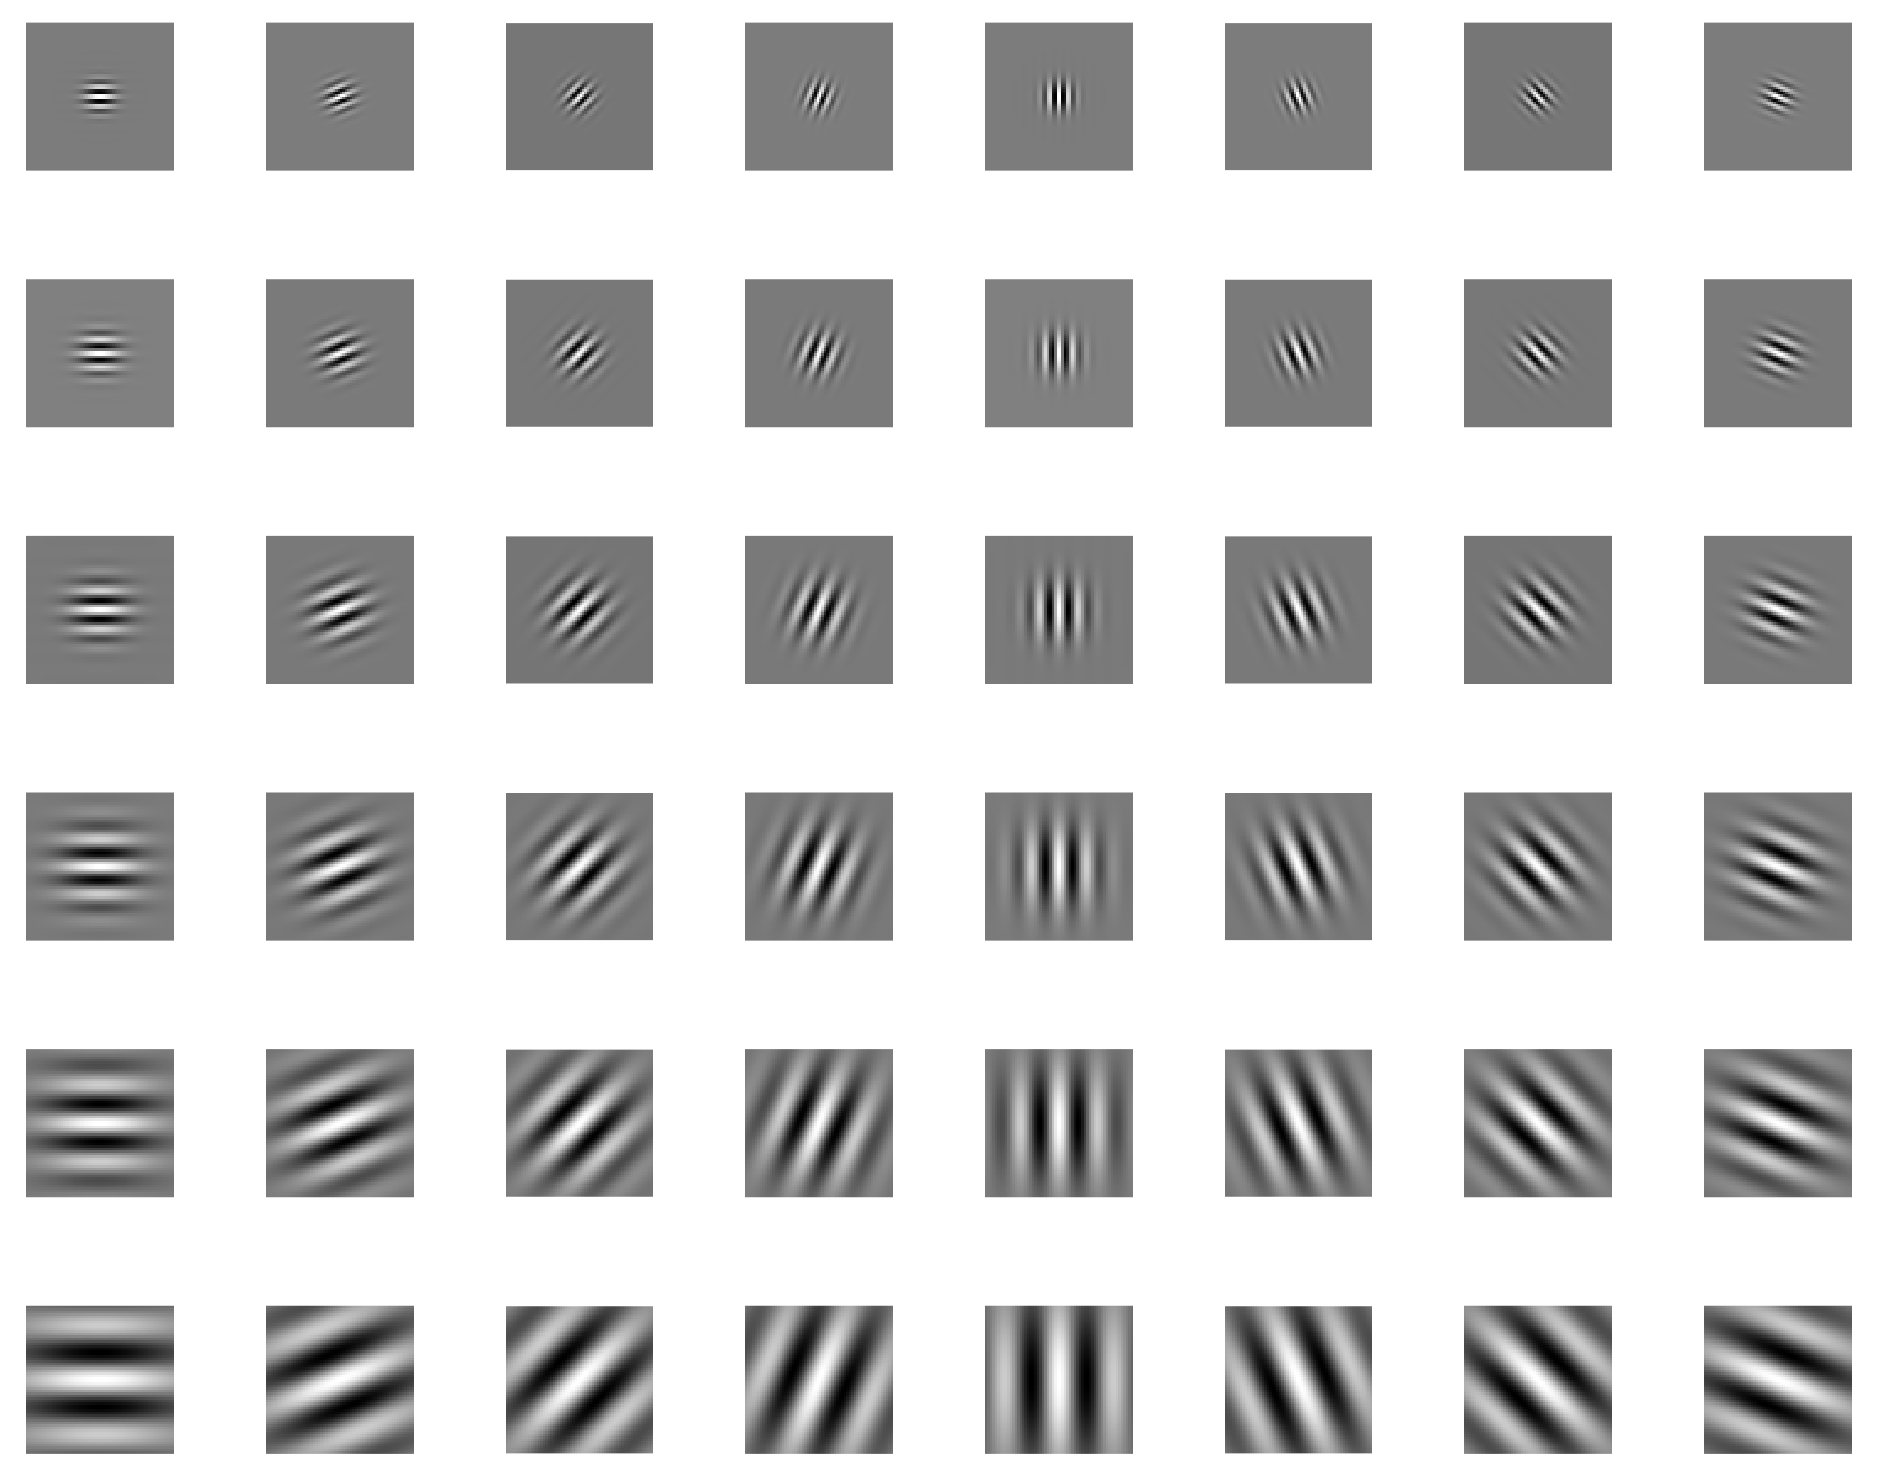
\includegraphics[height=7cm]{Gabor/gabor}
  \caption{不同参数下的Gabor滤波器}
  \label{fig:gabor}
\end{figure}

\subsubsection{局部二值模式}

局部二值模式(Local Binary Pattern, LBP)由Timo Objala等人在1994年提出~\cite{ojala1994performance},它是一种描述图像纹理特征的方法,该算法有灰度不变性和旋转不变性。局部二值模式的基本思想是用LBP值描述目标中每一个像素与其邻域像素之间的差别,然后通过统计整幅图像中的LBP值出现的频率来描述图像的特征。

通常LBP算子以每个像素点的$3 \times 3$邻域为窗口,假设中心点的灰度值为$g_{c}$,邻域点的值为$g_{0},g_{1},\dots,g_{7}$,则该区域内灰度值的联合分布可以表示为:
\begin{eqnarray}
T=t(g_{c},g_{0},\cdots,g_{7})
\end{eqnarray}

在计算图像中每一个像素点的LBP值时,将该点的灰度值作为阈值,$3 \times 3$邻域内另外8个点的灰度值分别与阈值比较,即:
\begin{eqnarray}
T=t(g_{c},g_{0}-g_{c},\cdots,g_{7}-g_{c})
\end{eqnarray}
由于联合分布$T$的取值比较广范,不利于描述,因此将灰度做差的结果用两个值来表示,即若中心阈值与其邻域像素点的灰度值之差值为负数,则将邻域中该点值记为0,否则记为1:
\begin{eqnarray}
T\approx t(s(g_{0}-g_{c}),s(g_{1}-g_{c}),\cdots,s(g_{7-g_{c}}))
\end{eqnarray}
其中$s$为符号函数,即$s(x)=\left \{ \begin{array}{ll} 1 & x>0\\ 0 & x<0 \end{array}\right.$。

给每个像素点乘以一个权值$2^{i}$并求和,就可以得到中心点周围区域纹理的描述值,称为LBP值,计算方法为:
\begin{eqnarray}
LBP_{8} = \sum^{7}_{i=0}s(g_{i}-g_{c})2^{i}
\end{eqnarray}

图~\ref{fig:lbpvalue}为LBP描述子的计算过程。
\begin{figure}[H] % use float package if you want it here
  \centering
  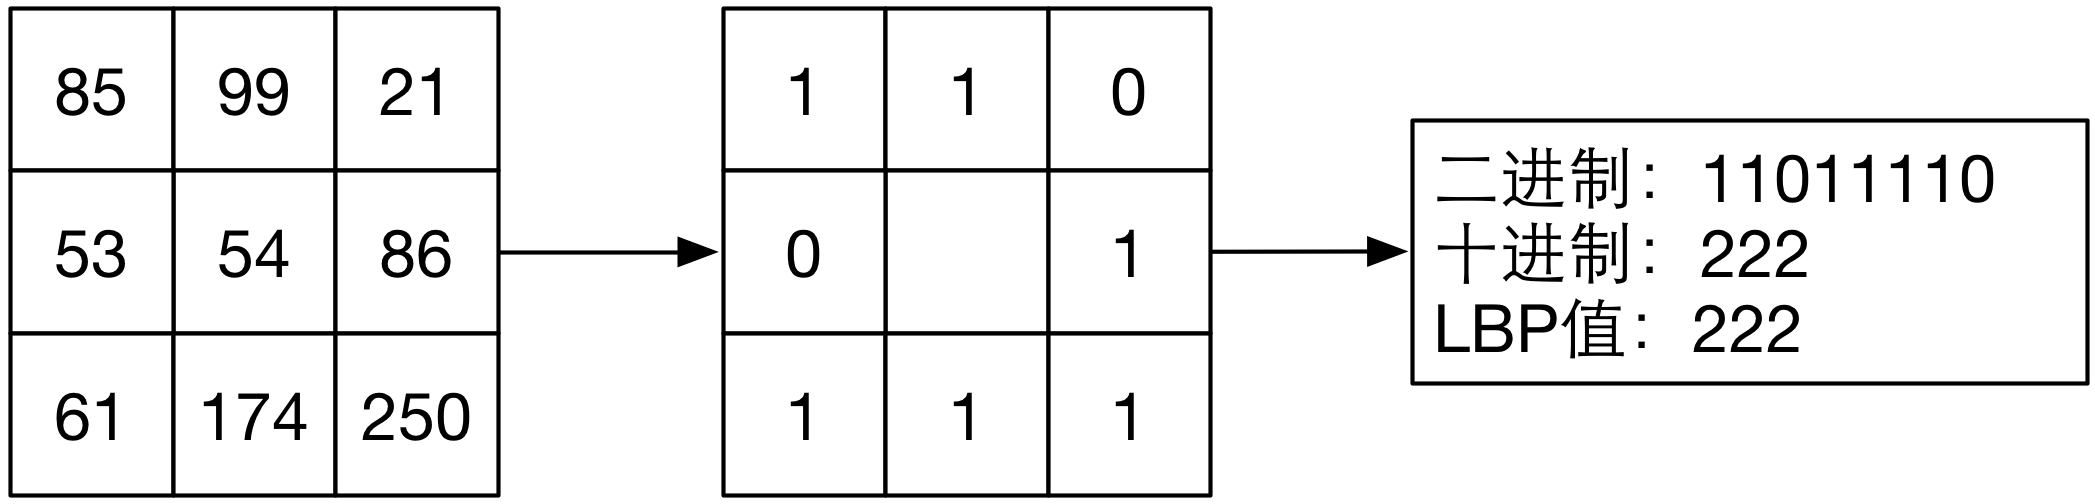
\includegraphics[height=2.5cm]{LBP/lbpvalue}
  \caption{计算LBP值}
  \label{fig:lbpvalue}
\end{figure}

经过上述过程后就能够得到图像中所有像素点的LBP值,然后用直方图统计图像中LBP值的出现频率,用其描述目标图像的纹理特征。综上采用LBP算法提取图像纹理特征的基本过程如下(如图~\ref{fig:lbpframework}):
\begin{figure}[H] % use float package if you want it here
  \centering
  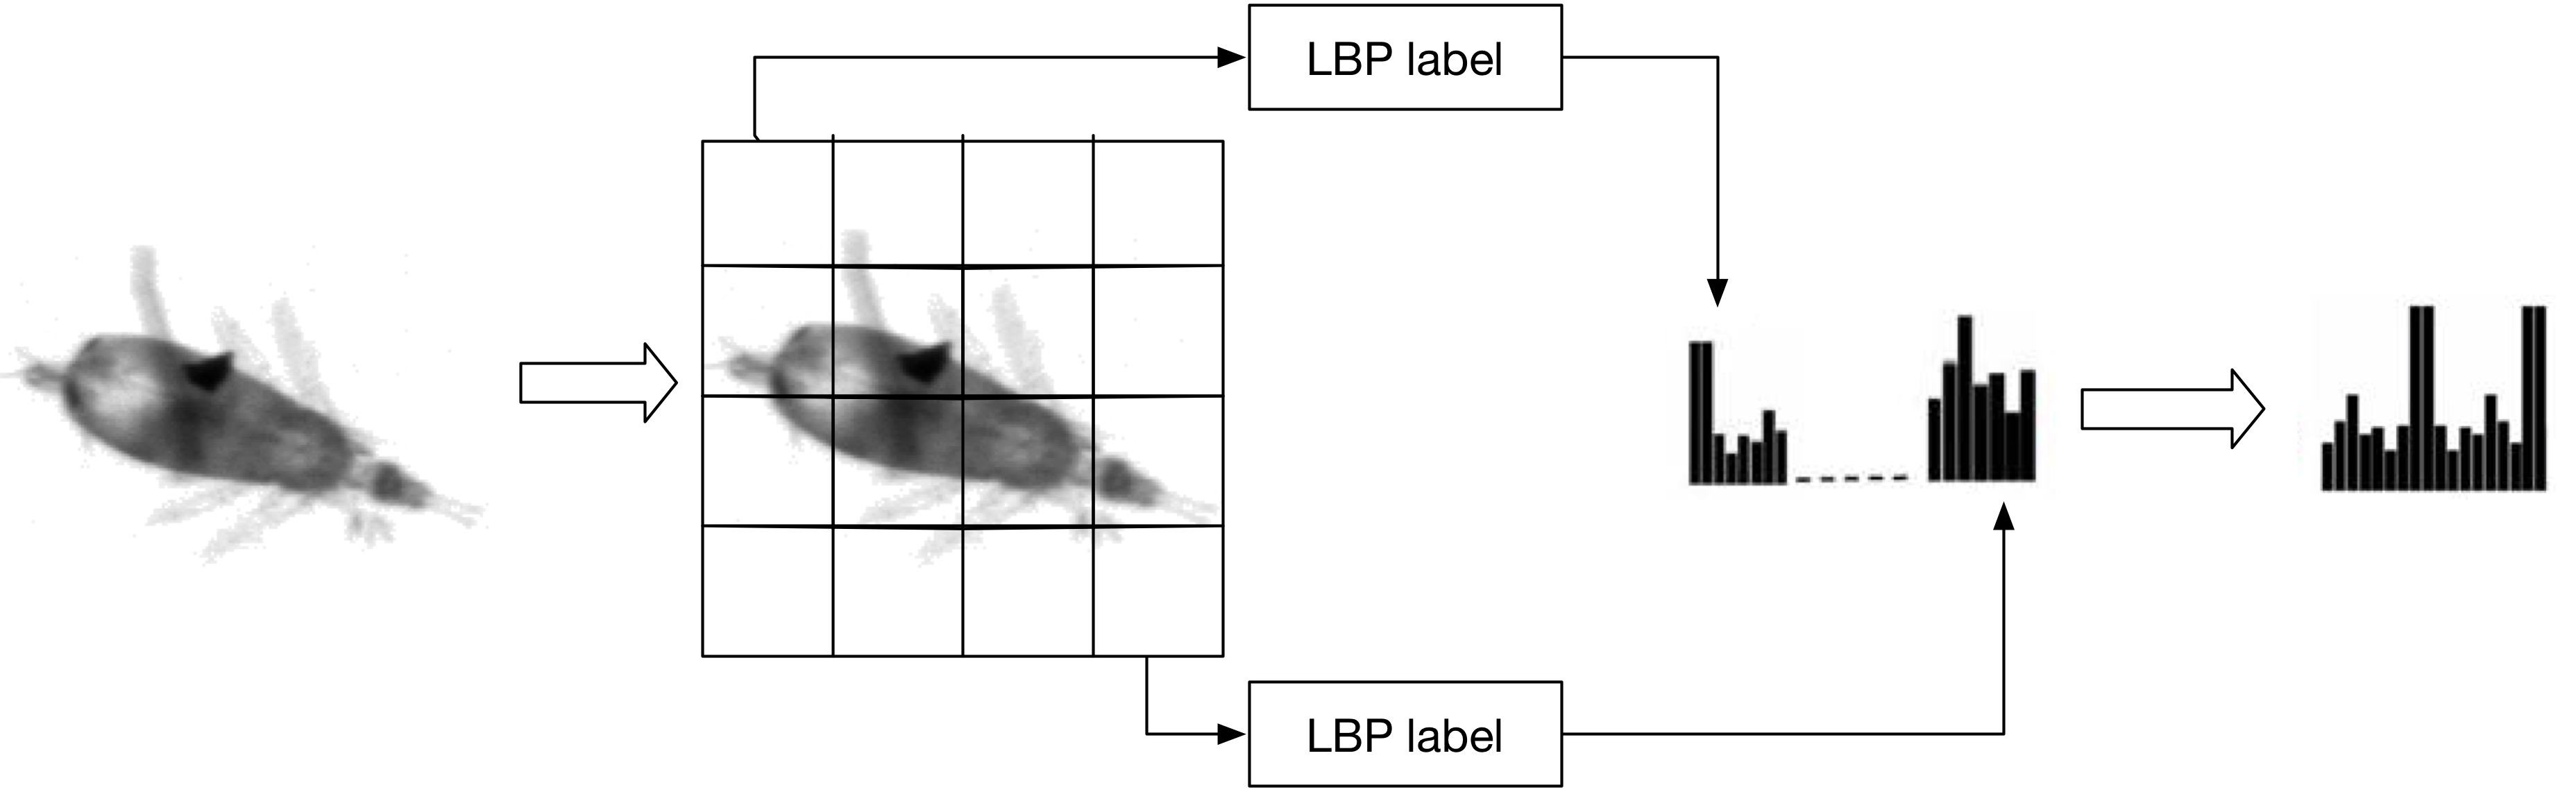
\includegraphics[height=4.5cm]{LBP/lbpframework}
  \caption{LBP特征提取过程}
  \label{fig:lbpframework}
\end{figure}
\begin{enumerate}
\item 先将图像分为多个子区域。
\item 分别计算子区域中每个像素点的LBP值。
\item 用直方图分别统计每个子区域内LBP值的出现频率,对每个子区域内的纹理特征进行描述。
\item 将一幅图像中全部子区域的直方图串联到一起,就可以得到描述该幅图像的LBP特征向量。
\end{enumerate}

\subsubsection{二元梯度轮廓}

二元梯度轮廓(Binary Gradient Contours, BGC)由Fernandez等人在2011年提出~\cite{fernandez2011image},是一种纹理特征描述算子。二元梯度轮廓与局部二值模式相似,它的基本思想是用BGC值对图像中每个像素与其$3 \times 3$邻域内像素梯度的差别进行描述,通过直方图统计BGC值的出现频率来描述图像的纹理特征。

二元梯度轮廓与局部二值模式的不同之处在于,二元梯度轮廓沿一定封闭路径计算中心像素的8邻域像素之间的梯度,然后使用0作为阈值,若两像素间梯度值大于0则记为1,否则记为0。在这个过程中,计算梯度的路径有多种,其中典型的三种路径如图~\ref{fig:BGCpath}所示。
\begin{figure}[h]
  \centering%
  \subcaptionbox{单程二元梯度轮廓\label{fig:BGC1}}%标题的长度,超过则会换行,如下一个小图。
    {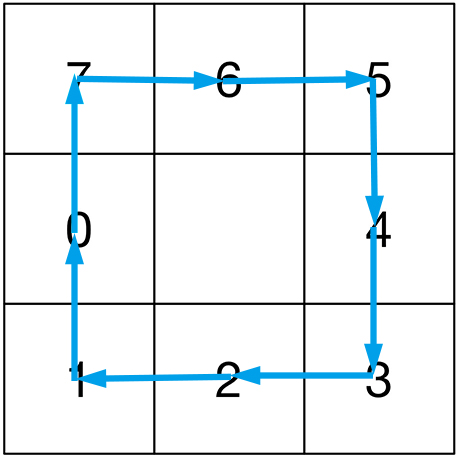
\includegraphics[height=3cm]{BGC/BGC1}}%
  \hspace{4em}%
  \subcaptionbox{双程二元梯度轮廓\label{fig:BGC2}}
      {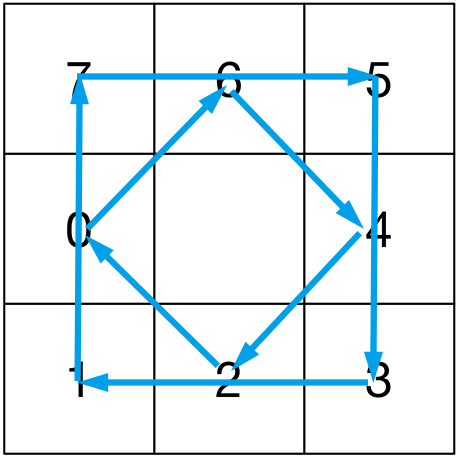
\includegraphics[height=3cm]{BGC/BGC2}}
  \hspace{4em}%
  \subcaptionbox{三程二元梯度轮廓\label{fig:BGC3}}
      {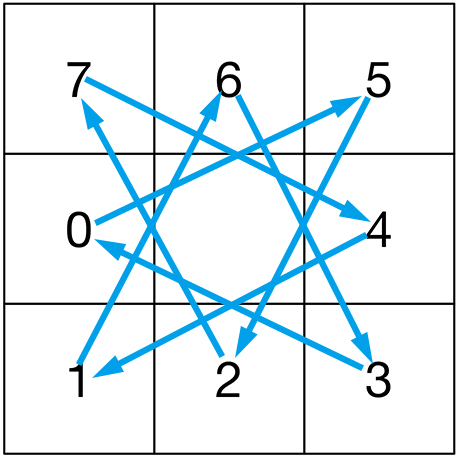
\includegraphics[height=3cm]{BGC/BGC3}}
  \caption{二元梯度轮廓的路径}
  \label{fig:BGCpath}
\end{figure}

图~\ref{fig:BGC1}由一条路径构成,叫做单程二元梯度轮廓(BGC1),公式如下:
\begin{eqnarray}
g_{1}=\left[ \begin{array}{l} s(I_{7}-I_{0}) \\ s(I_{6}-I_{7}) \\ s(I_{5}-I_{6}) \\ s(I_{4}-I_{5})\\ s(I_{3}-I_{4})\\ s(I_{2}-I_{3})\\ s(I_{1}-I_{2})\\ s(I_{0}-I_{1}) \end{array} \right]
\end{eqnarray}

图~\ref{fig:BGC2}中有两条路径,叫做双程二元梯度轮廓(BGC2),将两个回路计算的结果连接在一起来共同来表示每一个点:
\begin{eqnarray}
g_{2_{1}}=\left[ \begin{array}{l} s(I_{6}-I_{0})\\ s(I_{4}-I_{6})\\ s(I_{2}-I_{4})\\ s(I_{0}-I_{2}) \end{array} \right] , ~~~ g_{2_{2}}=\left[ \begin{array}{l} s(I_{7}-I_{1})\\ s(I_{5}-I_{7})\\ s(I_{3}-I_{5})\\ s(I_{1}-I_{3}) \end{array} \right]
\end{eqnarray}
\begin{eqnarray}
g_{2}=\left[ \begin{array}{l} g_{2_{1}}\\ g_{2_{2}} \end{array} \right]
\end{eqnarray}

同样,图~\ref{fig:BGC3}叫做三程二元梯度轮廓(BGC3),其表达式为:
\begin{eqnarray}
g_{3}=\left[ \begin{array}{l} s(I_{5}-I_{0})\\ s(I_{2}-I_{5})\\ s(I_{7}-I_{2})\\ s(I_{4}-I_{7})\\ s(I_{1}-I_{4})\\ s(I_{6}-I_{1})\\ s(I_{3}-I_{6})\\ s(I_{0}-I_{3}) \end{array} \right]
\end{eqnarray}

因此每个像素都可以获得一个8位二进制二元梯度轮廓值,求取图像点的各种二元梯度轮廓值的公式如下:
\begin{eqnarray}
BGC_{1} = w^{T}_{8}g_{1}-1\\
BGC_{2} = 15w^{T}_{4}g_{2_{2}}+w^{T}_{4}g_{2_{1}}-16\\
BGC_{3} = w^{T}_{8}g_{3}-1
\end{eqnarray}
其中,$w^{T}_{j}=[2^{j-1}  2^{j-2}  \dots  2^{1} 2^{0}]$。

根据以上式子可以求出图像中每个像素点的二元梯度轮廓值,然后用直方图统计图像中二元梯度轮廓值的出现频率。

\subsection{局部特征}

\subsubsection{内距离形状上下文}
\label{sec:onefig}

内距离形状上下文(Inner-Distance Shape Context, IDSC)由凌海滨在2007年提出~\cite{ling2007shape},它是对形状上下文方法(Shape Context, SC)~\cite{belongie2002shape}的一种改进。形状上下文是一种描述目标形状特征的方法,在2002年由Serge Belongie等人提出,该方法通过考察目标物体边缘上的点之间的空间位置关系来描述目标的形状特征,具体实现过程如下。

\begin{enumerate}
\item 首先提取目标物体(如图~\ref{fig:a})的轮廓边缘(如图~\ref{fig:a-edge})。由于轮廓上的像素点较多,需要从中采样n个点$P=\{p_1,\dots,p_n\}$来近似表示目标物体的轮廓(如图~\ref{fig:a-point})。在采集这n个点时要尽量保证采样点的重心和目标物体重心重合。
  \begin{figure}[H]
  \begin{minipage}{0.33\textwidth}
    \centering
    
\includegraphics[height=3cm]{IDSC/a}
    \caption{目标图像}
    \label{fig:a}
  \end{minipage}\hfill
  \begin{minipage}{0.33\textwidth}
    \centering
    
\includegraphics[height=3cm]{IDSC/a-edge}
    \caption{轮廓边缘}
    \label{fig:a-edge}
  \end{minipage}
  \begin{minipage}{0.33\textwidth}
    \centering
    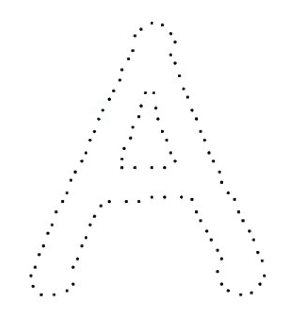
\includegraphics[height=3cm]{IDSC/a-point}
    \caption{采样点}
    \label{fig:a-point}
  \end{minipage}
  \end{figure}
\item 假设图~\ref{fig:a-point}中第i个采样点为$p_{i}$,则连接这个采样点$p_i$与其他$n-1$个点可以构成$n-1$个向量,这些向量可以表示该点$p_i$与轮廓上其他点间的相对位置关系。以$p_{i}$为原点建立对数极坐标系,如图~\ref{fig:a-log}所示,将图像中的坐标变换为极坐标,公式如下:
\begin{eqnarray}
r=\sqrt{(x-x_{0})^{2}+(y-y_{0})^{2}}, ~~~ \theta=arctan(\frac{y-y_{0}}{x-x_{0}})
\end{eqnarray}
其中$r$为欧式距离。将该极坐标系的半径$\log{r}$和测量角度$\theta$划分为5、12bin。这个对数空间将被分为48个区域,用直方图$h_{i}$统计边缘上其他$n-1$个点落在对数空间每个区域内的数量,即:
  \begin{eqnarray}
  h_{i}(k) = \#\{q \ne p_{i} : (q-p_{i})\in bin(k)\}
  \end{eqnarray}
其中,$k$为直方图中区域数量,直方图$h_{i}$就是点$p_i$的形状上下文,它可以表示点$p_i$与其他$n-1$个点之间的空间位置关系。图~\ref{fig:a-his}为图~\ref{fig:a-log}中点$p_{i}$的形状上下文。
  \begin{figure}[H]
  \begin{minipage}{0.5\textwidth}
    \centering
    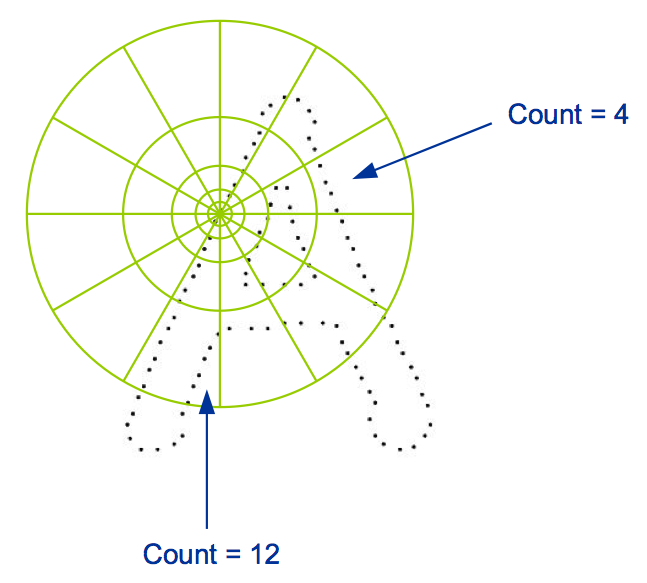
\includegraphics[height=4cm]{IDSC/a-log}
    \caption{对数极坐标系}
    \label{fig:a-log}
  \end{minipage}\hfill
  \begin{minipage}{0.5\textwidth}
    \centering
    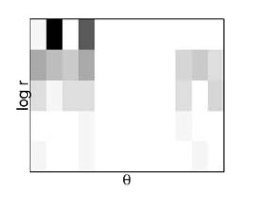
\includegraphics[height=3cm]{IDSC/a-his}
    \caption{形状直方图}
    \label{fig:a-his}
  \end{minipage}
  \end{figure}
\item 计算表示目标边缘上所有采样点之间位置关系的形状上下文,得到的所有点的结果构成了对目标物体形状的描述。
\end{enumerate}

在获得两个目标边缘上每一个采样点的形状上下文后,可以计算这两个目标上采样点之间的匹配关系,根据两目标上所有采样点之间的匹配程度可以得到两形状之间的相似程度,具体实现过程如下。

\begin{enumerate}
\item 假设形状$P$上的采样点为$p_i$和形状$Q$上的采样点为$q_j$,根据$C_{ij}=C(p_i,q_j)$可以计算这两点的匹配代价。
  \begin{eqnarray}
  C_{ij} \equiv C(p_{i},q_{j}) = \frac{1}{2}\sum^{n}_{k=1}\frac{[h_{i}(k)-h_{j}(k)]^{2}}{h_{i}(k)+h_{j}(k)}
  \end{eqnarray}
  其中$C_{ij}$为点$p_i$和$q_j$匹配的代价值,$h_{i}(k)$和$h_{j}(k)$表示点$p_i$和$q_j$的形状上下文。若$C_{ij}$值越小,则点$p_i$和$q_j$的形状上下文越相似,这两点的匹配程度越高~\cite{杨小娜2013基于形状上下文的目标形状识别与匹配}。
\item 对两个形状轮廓边缘上的采样点进行匹配时,必须将采样点一一对应,并且使全部点的匹配代价值的和最小,即
  \begin{eqnarray}
  H(\pi) = \sum_{i}C(p_{i},q_{\pi(i)})
  \end{eqnarray}
  其中$\pi$是一种置换,约束条件是实现采样点的一一对应匹配,使用匈牙利算法可以解决。
\item 使用薄板样条(Thin Plate Spline, TPS)模型表示弹性坐标转换。用两个独立的TPS函数来模拟坐标的变换,从第一个形状的任意位置映射到第二个形状。
  \begin{eqnarray}
  T(x,y)=(f_{x}(x,y),f_{y}(x,y))
  \end{eqnarray}
\item 计算两个形状之间的距离:
  \begin{multline}
  D_{sc}(P,Q)=\frac{1}{n}\sum_{p\in P}arg \min_{q\in Q}C(p,T(q))+\\
  \frac{1}{m}\sum_{q\in Q}arg \min_{p\in P}arg \min_{p\in P}C(p,T(q))
  \end{multline}
  其中$T$为形状$Q$上的点到$P$的TPS变换。
\end{enumerate}

内距离形状上下文是在形状上下文的基础上进行改进,即在内距离形状上下文中统计采样点的位置关系时使用内距离代替了形状上下文中的欧式距离。内距离是指目标轮廓上的两点位于其形状内部距离的最短值,如图~\ref{fig:innerdistance}所示。内距离形状上下文相对应形状上下文而言,对目标的非刚性变化更加敏感,描述局部特征具有更好的鲁棒性。
\begin{figure}[H] % use float package if you want it here
  \centering
  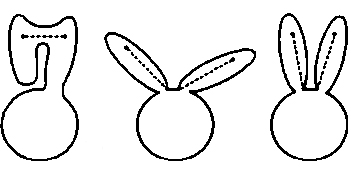
\includegraphics[height=2.5cm]{IDSC/innerdistance}
  \caption{内距离}
  \label{fig:innerdistance}
\end{figure}

在本文研究中使用内距离形状上下文来提取浮游生物的形状特征,主要思想是通过内距离形状上下文计算待识别样本形状与已知浮游生物形状模板之间的相似度来描述形状特征,具体实现过程如下。

\begin{enumerate}
\item 针对每个数据集,选取$n$张不同形状的浮游生物图像,通过人工标注的方法得到这些图像中浮游生物的形状真值图作为形状模板。
\item 采用内距离形状上下文计算数据集中所有浮游生物图像和n张形状模板之间的距离,每张图像都会得到$n$个距离,这些距离表示每张图像的形状与形状模板之间的相似程度。针对每幅图像计算得到的$n$个值可以构成一个$n$维向量,这个向量可以描述该目标形状特征。
\end{enumerate}


\subsubsection{方向梯度直方图}

方向梯度直方图(Histogram of Oriented Gradients, HOG)由Dalal等人在2005年提出~\cite{dalal2005histograms},是一种特征描述方法,具有良好的旋转和平移一致性,被广泛的用于目标检测中。方向梯度直方图的基本思想是通过描述局部区域内的灰度梯度来表示图像的特征,其算法过程如下:

\begin{enumerate}
\item 先将图像进行灰度化,然后采用Gamma校正和灰度归一化处理获得的灰度图像。由于采集的图像受到光照变化、阴影的影响,通过Gamma校正来调节对比度,减少光照等其他因素的影响。

  Gamma压缩公式为:
  \begin{eqnarray}
  I(x,y) = I(x,y)^{gamma}
  \end{eqnarray}
\item 采用梯度算法计算所获得的灰度图像的梯度,获得目标的轮廓信息。

  在计算图像梯度时,通常采用一阶微分模板$[-1,0,1]$求梯度,对图像上任意一点用该模板可以得到垂直和水平方向上的梯度:
  \begin{eqnarray}
  G_{x}(x,y)=H(x+1,y)-H(x-1,y)\\
  G_{y}(x,y)=H(x,y+1)-H(x,y-1)
  \end{eqnarray}

  梯度的幅值和方向计算公式为:
  \begin{eqnarray}
  G(x,y)=\sqrt{G_{x}(x,y)^{2}+G_{y}(x,y)^2}
  \end{eqnarray}
  \begin{eqnarray}
  \theta(x,y)=\tan^{-1}\frac{G_{y}(x,y)}{G_{x}(x,y)}
  \end{eqnarray}

\item 将图像分为Cell(即单元),每个单元都由若干个像素组成。%,如$6 \times 6 \frac{\textrm{像素}}{\textrm{单元}}$。
\item 用直方图对图像中所有单元中的梯度方向加权统计。梯度的范围为0至360度,将其分为n份,统计梯度方向落在每份区域内的梯度加权值。
\item 每几个单元组成一个块(Block),将重叠单元块进行标准化,然后把块中所有单元的直方图向量组合起来得到的向量就是该块的特征描述符。
\item 图像中所有块的特征向量组合到一起就得到了该幅图像的HOG特征。
\end{enumerate}

在本文实验中,使用方向梯度直方图来提取浮游生物的形态特征,在实验中将图像处理为$256 \times 256$,将单元大小设定为$32 \times 32$。

\subsubsection{尺度不变特征变换}

尺度不变特征变换(Scale Invariant feature transform, SIFT)是一种局部特征描述算法,在1999年由Lowe提出\cite{lowe1999object},后来又进行了完善。SIFT有旋转不变和尺度不变等性质,并且被广泛的用于目标识别、目标匹配等领域中。SIFT算法的基本思想是提取图像中的高健壮性的特征点,通过对这些特征点的描述实现对图像中目标特征的描述,该算法的基本实现如下:

\begin{enumerate}
\item 采用高斯函数和图像下采样构建多尺度空间。

  将原图像与不同参数的高斯函数卷积可以实现在不同尺度下对图像滤波:
  \begin{eqnarray}
  L(x,y,\sigma) = G(x,y,\sigma) \ast I(x,y)
  \end{eqnarray}
  其中$I(x,y)$表示原始图像,$L(x,y,\sigma)$表示滤波后得到的图像,$G(x,y,\sigma)$表示高斯函数,
  \begin{eqnarray}
  G(x,y,\sigma)=\frac{1}{2\pi \sigma^{2}}e^{-\frac{x^{2}+y^{2}}{2\sigma^{2}}}
  \end{eqnarray}
  上式中$x,y$是空间坐标,参数$\sigma$决定着对图像滤波程度。为了有效的确定图像中的关键点,将图像与两个相邻尺度高斯函数的卷积结果做差,从而构建高斯差分尺度空间(DOG):
  \begin{multline}
  D(x,y,\sigma)=(G(x,y,k\sigma)-G(x,y,\sigma))\ast I(x,y) \\
  = L(x,y,k\sigma)-L(x,y,\sigma)
  \end{multline}

  采用以上方法来建立图像金字塔。图~\ref{fig:dog}为图像金字塔的结构,从中可以看出每个金字塔包括i个子八度(Octave),并且每个子八度有包括s层。子八度是通过对图像下采样得到i个不同大小的图像(即不同尺度的图像,每次采样得到的图像都为原图的四分之一)组成的。每个子八度中的s(通常为3至5)层是使用高斯函数对图像进行不同程度滤波得到的。
  \begin{figure}[H] % use float package if you want it here
  \centering
  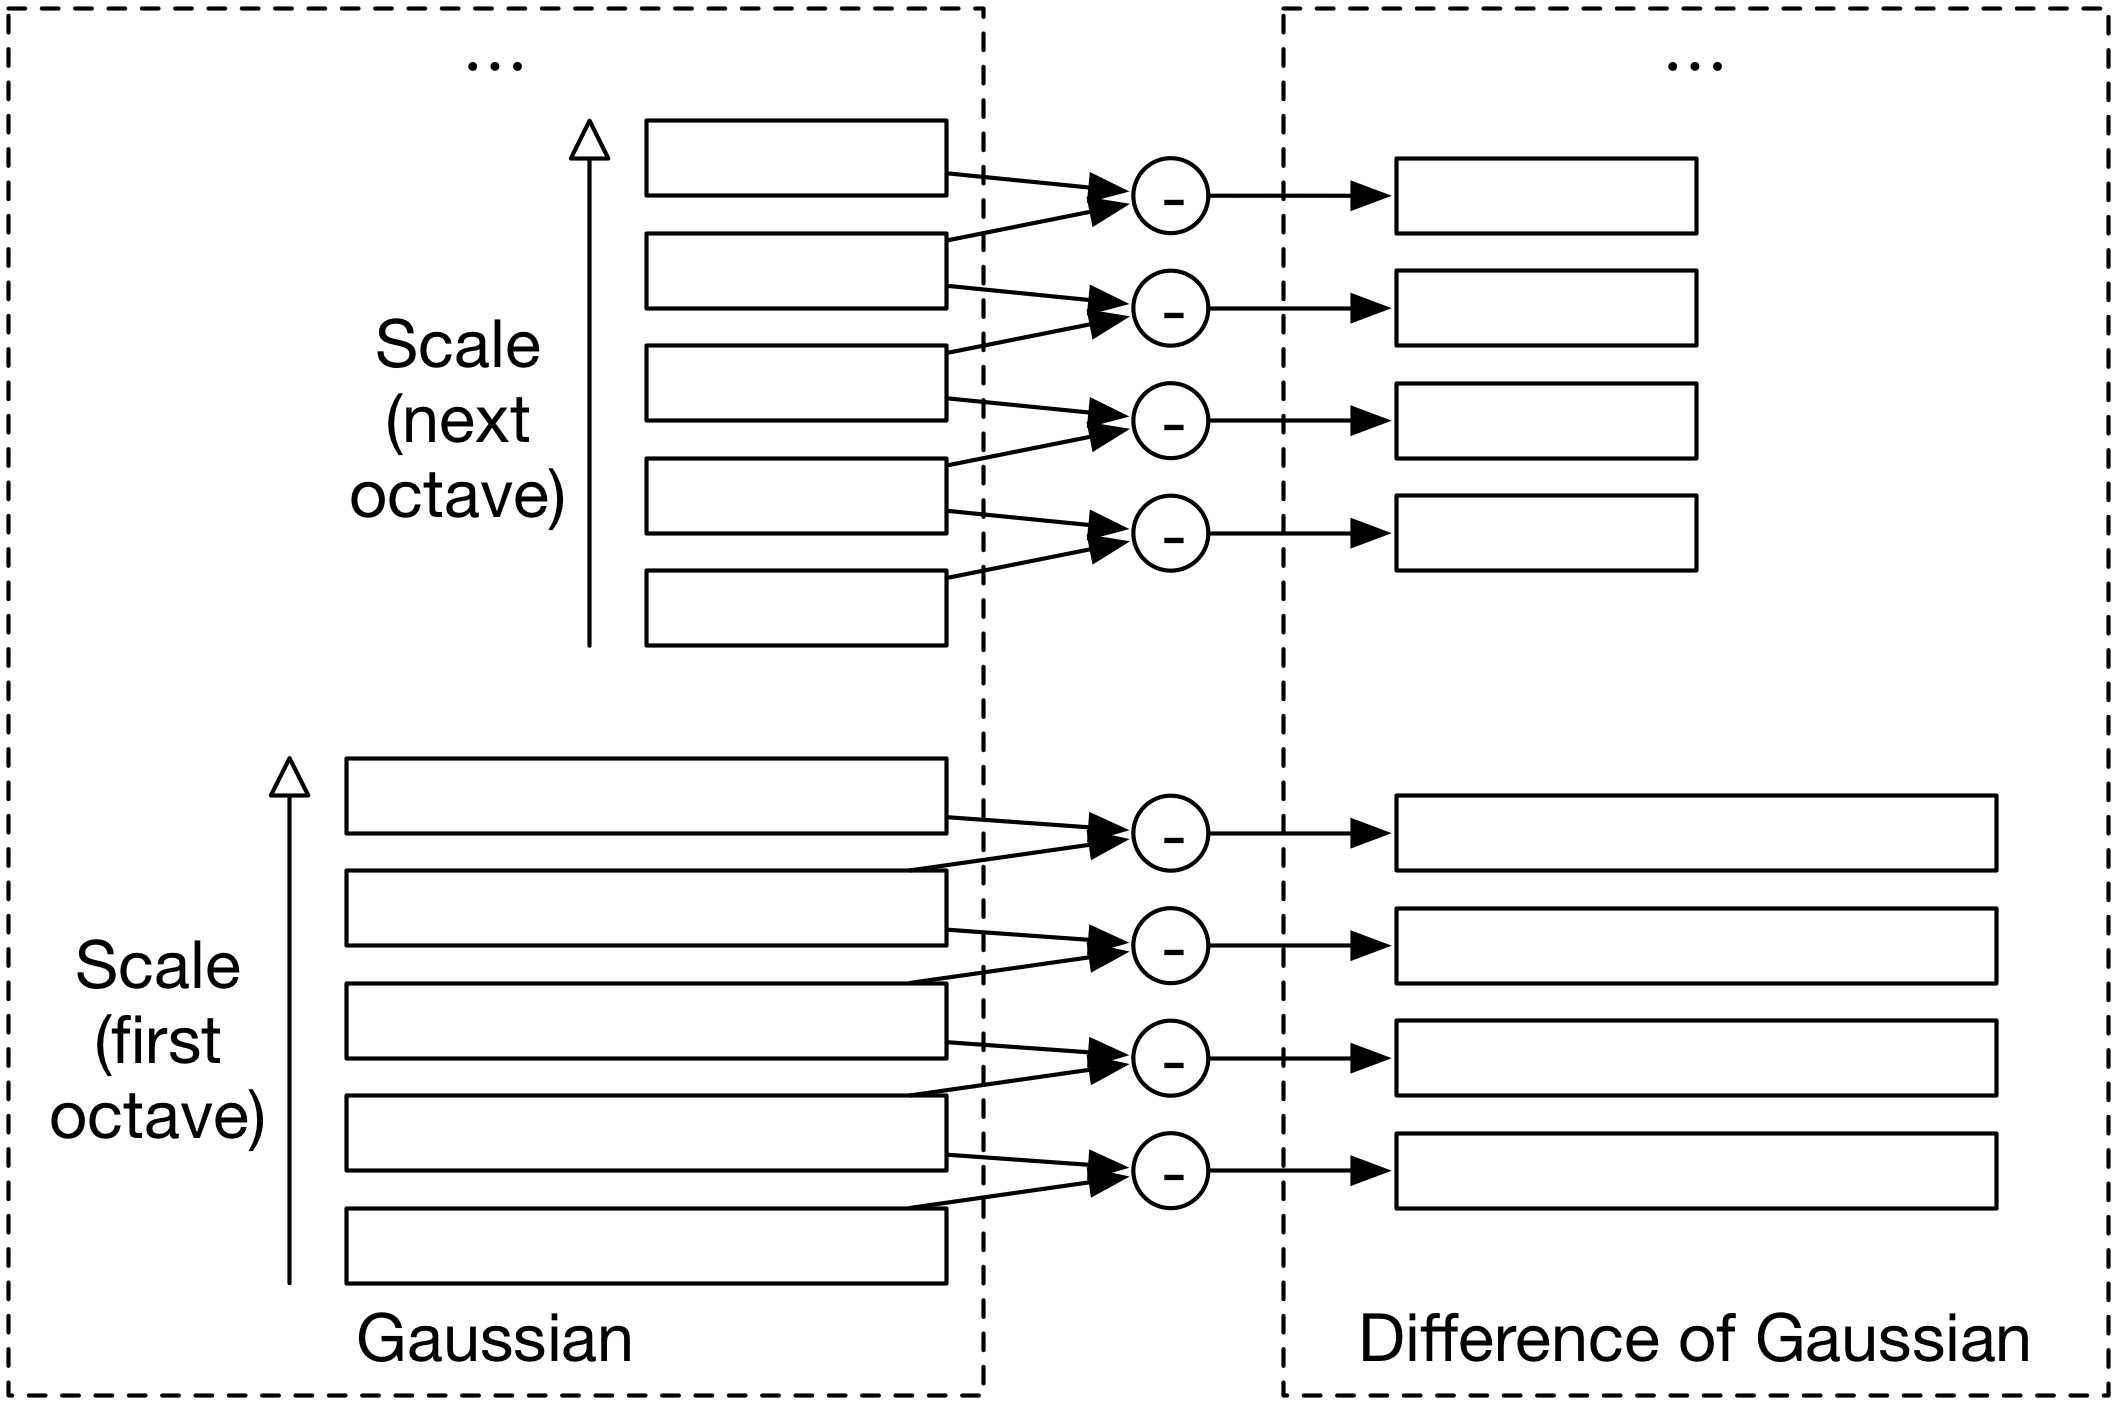
\includegraphics[height=6cm]{sift/DOG}
  \caption{图像金字塔}
  \label{fig:dog}
  \end{figure}

\item 确定图像中的极值点。在DOG空间中确定极值点时,将每一个点与其空间中的邻域比较,观察该点是否是其邻域中的最大值或最小值点。如图~\ref{fig:neg}所示,每一个点的邻域包括其所在层的8邻域以及上下两层的9邻域,所以在确定极值点时每个点要与其空间邻域中的26个相邻点比较。
  \begin{figure}[H] % use float package if you want it here
  \centering
  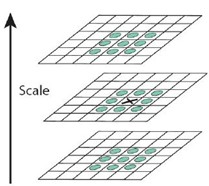
\includegraphics[height=4cm]{sift/neg}
  \caption{检测尺度空间的极值点}
  \label{fig:neg}
  \end{figure}
\item 精确定位特征点。得到的极值点中会存在着一些对比度较低和边缘响应点,将它们去除后保留下来的点就是特征点,即关键点。

  在对关键点的位置和尺度进行精确定位时,采用拟和三维二次函数将关键点中对比度较低的点和边缘相应点去除,从而增强特征描述的稳定性和抗噪能力,实现过程如下。

  尺度空间的泰勒展开式如下:
  \begin{eqnarray}
  D(x)=D+\frac{\partial D^{T}}{\partial x}x+\frac{1}{2}x^{T}\frac{\partial^{2}D}{\partial x^{2}}x
  \end{eqnarray}
  对上式中$x$求导,且让导数为零可得到:
  \begin{eqnarray}
  \hat{x} = -\frac{\partial^{2}D^{-1}}{\partial x^{2}}\frac{\partial D}{\partial x}
  \end{eqnarray}
  将上式代入$D(x)$得:
  \begin{eqnarray}
  D(\hat{x})=D+\frac{1}{2}\frac{\partial D^{T}}{\partial x}\hat{x}
  \end{eqnarray}
  若$|D(\hat{x})| \ge 0.03$,则该关键点保留,否则将其去掉。

  另外还要排除图像中边缘上的关键点,位于图像横跨边缘处的关键点主曲率较大,而在竖直边缘处点的主曲率较小~\cite{陈健斌2012图像特征提取及其相似度的研究和实现},通过这一性质来排除无用的关键点。主曲率可以通过Hessian矩阵求得:
  \begin{eqnarray}
  H=\left[ \begin{array}{ll} D_{xx} & D_{xy}\\ D_{xy} & D_{yy} \end{array} \right]
  \end{eqnarray}
  若H的特征值为$\alpha, \beta$,其中$\alpha$较大,$\beta$较小,则
  \begin{eqnarray}
  Tr(H)=D_{xx}+D_{yy}=\alpha + \beta\\
  Det(H)=D_{xx}D_{yy}-(D_{xy})^{2}=\alpha\beta
  \end{eqnarray}
  因此,令$\alpha = \lambda\beta$,则:
  \begin{eqnarray}
  \frac{Tr(H)^{2}}{Det(H)}=\frac{(\alpha+\beta)^{2}}{\alpha\beta}=\frac{(\gamma\beta+\beta)^{2}}{\gamma\beta^{2}}=\frac{(\gamma+1)^{2}}{\gamma}
  \end{eqnarray}

\item 确定关键点方向参数。在得到图像中关键点后,为了使其具有旋转不变性,需要确定它们的主方向。若关键点邻域内其他像素点$(x,y)$的梯度幅值和方向如下:
  \begin{eqnarray}
  m(x,y)=\sqrt{(L(x+1,y)-L(x-1,y))^{2}+(L(x,y+1)-L(x,y-1))^{2}}
  \end{eqnarray}
  \begin{eqnarray}
  \theta(x,y)=\tan 2\frac{L(x,y+1)-L(x,y-1)}{L(x+1,y)-L(x-1,y)}
  \end{eqnarray}

  用直方图对关键点相邻区域内所有像素点的梯度方向进行统计,其横坐标的范围为0至360度。关键点的方向就是梯度直方图的峰值所表示的梯度方向。
\item 对关键点进行描述。在确定完关键点方向后,以关键点方向为轴建立坐标系生成关键点的特征描述子,具体过程如下:
  \begin{enumerate}
  \item 首先,将关键点作为中心点,取其$16\times16$邻域,然后计算其中所有像素点的梯度。
  \item 将这个邻域分为16个$4\times4$的子区域,用8个bin的直方图加权统计每个子区域内像素的梯度方向。
  \item 将得到的所有直方图结合在一起可以得到一个128($16 \times 8$)维的向量,该向量就是对关键点的特征描述。
  \end{enumerate}
\end{enumerate}

SIFT算法通过提取并描述图像中的关键点来表示图像的特征。SIFT对不同图像提取得到的关键点数量是不同的,每幅图可能包含成百上千个。因此,在进行目标识别过程中,采用SIFT特征来描述每幅图像时得到特征向量数量各不相同,特征点数量越多特征向量越多,分类计算量也越大。因此,用SIFT算法进行图像分类时通常要用到Bag of Words模型。

Bag of Words模型也称为“词袋”,最初用于文本分类中,基本思想是假设两个文本,不考虑其中的语法、词序等,把文本看成一系列词汇的组合,将构成这两个文本的所有词汇放在一起,得到一个词袋,然后这两个文本又可以用这个词袋中的词汇重新描述。同理,将SIFT算法用于目标识别时,每幅图像可以看成一个文本,描述图像中每个特征点的特征向量看做为词汇,将所有图像中所有特征点的特征向量放在一起构成一个词袋,然后用这个词袋重新对每幅图像的特征进行描述。这样得到的描述每幅图像的特征向量不仅规整,而且减少了计算量,大大提高了计算效率。使用BOW模型描述图像特征的基本步骤如下:
\begin{enumerate}
\item 若数据集中有n张图像,采用SIFT算法提取所有图像中的特征点,并得到每一个特征点的128维特征向量。
\item 将SIFT提取的n张图像的所有特征点放在一起,采用K-means对这些特征点聚类,假设一共聚为m类。
\item 每个类别分别有一个聚类中心,计算每幅图像中所有特征点到这m个中心的距离,将每个特征点分别归到距其最近中心所属的类别中去,可以使用直方图向量统计每幅图像中特征点在m个类别中出现频率,该向量就是对图像特征的描述。
\end{enumerate}

在本文研究中,采用SIFT提取数据集中全部图像的特征点,然后用K-means算法将所有特征点聚为100类,分别描述每幅图像中特征在100类中出现的频率,因此每幅图像的特征可以得到一个100维的特征向量。

\section{浮游生物特征选择}
\label{sec:featureselection}

特征选择是指去除特征中的冗余部分,降低特征维数,保留有用的特征,同时提高分类的效率和准确率。在分类识别中,有效的特征信息是训练优秀分类器的重要因素,特征中的冗余部分不仅会影响分类的结果~\cite{姚旭2012特征选择方法综述},还会降低效率,因此在机器学习过程中对特征进行选择是至关重要的。

到目前为止,已经有很多研究者对特征选进行研究定义:在1992年Kria和Rendell~\cite{Kira1992The}提出特征选择是找到可以对目标进行识别的最小特征集合;后来John等人~\cite{John1998Irrelevant}提出减少特征维数是在能够提高或不要降低准确率的前提下进行;Koller等人~\cite{Koller2000Toward}认为在选择最小的特征集合时确保分类结果的分布与原始类分布相似;后来Dash等人\cite{Dash1997Feature}结合上述观点,将特征选择定义为在不降低分类准确度且不改变类比分布的情况下保留尽可能小的特征集合。

特征选择方法的基本步骤是:先生成候选的特征子集,然后对其进行评价,判断选择结果是否符合停止准则,若符合则对检验结果,否则重新生成候选特征子集。目前特征选择的方法有很多,按照搜索测量和评价标准的不同将其分类。

\subsection{按搜索测量进行特征选择的方法}

根据特征选择方法在选取子集时使用的搜索策略将其分为:全局最优、随机搜索和启发式搜索,下面对这三种方法分别进行介绍。

\subsubsection{基于全局最优搜索策略的特征选择方法}

分支界定是基于全局最优搜索策略的特征选择方法中可以获得最优结果的唯一算法~\cite{姚旭2012特征选择方法综述},该算法的基本思想是:将所有可能的特征选择组合构成一个树状结构,按照特定的规则对树进行搜索,使搜索过程尽可能得到最优解而不必须遍历整个树。使用这种方法的前提是需要准则判据对特征有单调性,但是在处理高纬度特征时,该算法的时间复杂度较高。所以,基于全局最优搜索策略的算法虽然可以获得最优结果,但是很难被广泛的使用。

\subsubsection{基于随机搜索策略的特征选择方法}

基于随机搜索策略的特征选择方法通过有一定智能的随机搜索策略实现,在计算过程中该方法结合了特征选择与粒子群优化算法、模拟退火算法、遗传算法等,将采样和概率推理看做选择的基本,按照每个特征分类时的有效性,给它们分别赋予一个权值,然后按照设定或自适应阈值确定对分类有用的特征。若某个特征的权重超过该阈值,则这个特征便是有用的~\cite{宁永鹏2014高维小样本数据的特征选择研究及其稳定性分析}。

\subsubsection{基于启发式搜索策略的特征选择方法}

利用问题的启发信息作为引导,并进行搜索的方法称为启发式搜索,该方法可以降低问题的复杂度,并且减少搜索的范围。在特征选择过程中全局最优的搜索算法计算量可能很大,因此出现了以启发式搜索策略为基础的特征选择算法,该方法可以分为以下几种:单独最优特征组合、浮动搜索、增l去r选择方法、序列前向选择方法、广义序列前向选择方法、序列后向选择方法、广义序列后向选择方法、广义增l去r选择方法。虽然启发式搜索策略的效率较高,但是是以牺牲全局最优为代价。

\subsection{按评价准则进行特征选择的方法}

在特征选择过程中,对所选择特征好坏的有不同的评价方法。根据评价方法是否依赖于后续的学习算法能够将特征选择方法分为两种:过滤式(Filter)和封装式(Wrapper)~\cite{宁永鹏2014高维小样本数据的特征选择研究及其稳定性分析}。过滤式特征选择独立于之后的学习算法,通常情况下可以直接使用训练数据的统计性能对特征进行评估,虽然计算效率较高,但是之后使用学习算法得到的结果和评估结果可能相差较大。封装式方法需要用后续的学习算法来对特征子集进行评价,因此结果与之后学习算法相差较小,但是计算量大。下面分别介绍这两种方法。

\subsubsection{过滤式评价准则的特征选择方法}

过滤式特征选择具有较高的效率,该方法通常用评价准则来增加特征与类别之间的相关性,去除掉不相关的杂质特征,优化特征子集,就像过滤器一样。根据评价准则可以将过滤式方法分成:一致性度量、依赖性度量、信息度量以及距离度量。这些方法的一个主要问题在找到的最优特征子集的规模往往较大,其中会包含一些噪声,但计算效率较高。

\subsubsection{封装式评价准则的特征选择方法}

封装式方法需要用之后的学习算法对选取的特征进行评估,将学习算法看做特征选择的一部分,按照学习得到的分类器性能进行特征选择。采用封装式方法进行特征选择时,用选取的特征集合来训练分类器,获得分类器的分类准确率可以作为评价所选特征重要性的标准。基于封装式的特征选择方法的计算速度要比基于过滤式的方法慢,但是它选择得到的特征子集维数较小,如今该方法在特征选择领域有较为广泛的应用。

在本文实验中,由于提取的图像特征种类丰富并且维数较高,因此其中会包含部分的冗余特征,这些特征不仅不利于分类准确率的提高,还降低了计算效率,因此在特征提取后又进一步进行了特征选择,采用的特征选择算法为基于封装式评价准则的特征选择算法。

\section{本章小结}

浮游生物种类繁多,类别相近的生物之间形态特征相差较小,而浮游植物和动物之间的差异又较大,这些特点增加了浮游生物分类的难度,因此需要全面充足的特征信息对浮游生物的形态特征进行描述。本章介绍了根据浮游生物形态特征选用的特征提取方法,包括:几何灰度统计特征;局部二值模式、二元梯度轮廓、Gabor滤波器等纹理特征描述算法;内距离形状上下文、尺度不变特征变换等局部特征描述算法。这些特征提取算法可以对浮游生物的大小、形状、灰度、纹理等信息全面的描述。

由于提取的浮游生物特征较多,在提取的特征中可能存在冗余或不相关的信息,这些信息的存在不利于分类性能和准确率的提高,因此我们引入了基于封装式评价准则的特征选择方法对提取的特征进行筛选,去除冗余信息,降低维数,进而可以提高的分类器的泛化能力和整体性能。











\chapter{基于多核学习的浮游生物图像分类研究}

使用多核学习融合多种不同特征可以更好的发挥每种特征在分类过程中的积极作用。本章首先对多核学习的理论进行介绍;然后介绍设计的分类系统;最后,设计一系列对比实验分析分类系统的性能,并根据实验结果对分类系统性能进行评价。

\section{多核学习理论}

在图像分类识别过程中采用多种特征对目标进行描述有利于提高分类的准确率,而在这个过程中如何融合多种特征的方法又是人们关注的重点。通常特征融合算法可以分为决策级融合、特征级融合和数据级融合三类。数据级融合是将未加工的图像信息结合来得到更丰富的信息,常用的算法有主成分分析、线性加权法等。特征级融合是通过选择去除多余的特征,然后融合不相关的特征,例如聚类分析法、信息熵法等。决策级融合是将多个分类器结合,常用算法有贝叶斯融合、模糊聚类法、多核学习算法等。在本文中使用多核学习算法对提取的多种特征进行融合并训练分类器。

多核学习属于多视角学习。我们经常使用的支持向量机是一种单核学习方法,往往不能满足处理多种特征的需求,而多核学习为融合几种不同的核进行训练的学习方法,可以充分发挥每种特征在分类过程中的积极作用。下面以支持向量机为基础介绍核函数的原理,进而介绍多核学习的理论和方法。

\subsection{支持向量机}

早在1995年Cortes等人提出了支持向量机(Support Vector Machine, SVM)~\cite{Cortes1995Support},该方法属于监督学习,常用于目标分类和回归分析。支持向量机以VC维理论和结构风险最小化原理为基础,基本思想是在特征空间中构建一个最大间隔分类超平实现对未知样本的分类。因此,该方法适合处理二分类和回归问题,被普遍的应用在统计分类和回归分析中。

\subsubsection{线性可分支持向量机}

线性可分支持向量机是指训练样本在特征空间中线性可分,可以找到一个线性超平面将不同类别的样本完全正确的分开。设给定的样本为$(x_{1},y_{1}),\cdots,(x_{n},y_{n})$,其中$x_{i}\in X = R^{n}$,$y_{i}\in \{1,-1\}$,$x_{i}$为第$i$个样本的特征向量,$y_{i}$为第$i$个样本所属的类别。支持向量机对样本进行分类是通过在特征空间中找到最大间隔超平面将不同类别的样本划分开,如图~\ref{fig:svm}所示,超平面的方程可以表示为:
\begin{figure}%[H] % use float package if you want it here
  \centering
  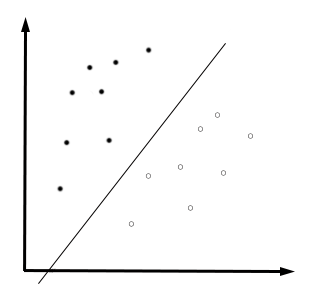
\includegraphics[height=4cm]{MKL/svm}
  \caption{SVM分类超平面}
  \label{fig:svm}
\end{figure}
\begin{eqnarray}
w^{T}x+b=0
\end{eqnarray}
其中,$w$表示垂直于超平面的向量,$b$表示超平面的截距,该分类问题的决策函数为:
\begin{eqnarray}
f(x)=s(w^{T}x+b)
\end{eqnarray}
若$f(x_{i})$大于0,则$x_{i}$为类别$1$,否则为类别$-1$。

若要找到最大间隔超平面,则需要计算样本到超平面的距离。通常$|wx_{i}+b|$可以表示样本点$i$距离超平面的远近,而$wx_{i}+b$与$y_{i}$的符号相同,因此可以用$\hat{\gamma}=y(wx+b)$表示样本到分类平面的距离,这就是函数间隔。然而在选择超平面时,$w$和$b$等比例的变化并不会改变超平面,但是却会改变函数间隔。因此,引入几何间隔:
\begin{eqnarray}
\tilde{\gamma}=\frac{\hat{\gamma}}{||w||}
\end{eqnarray}

一个超平面的几何间隔是所有训练样本距离该超平面的几何间隔中的最小值,而支持向量机得学习目标是要在特征空间中找到一个超平面,使其几何间隔最大。对线性可分的样本集来说,其线性可分超平面有很多个,然而几何间隔最大的分类超平面就一个。

若要找到最大间隔分类超平面,需要令几何间隔最大,即:
\begin{eqnarray}
\max \tilde{\gamma}=\max\frac{\hat{\gamma}}{||w||}=\max\frac{y(w^{T}x+b)}{||w||}
\end{eqnarray}

其中函数间隔$\hat{\gamma}$的大小并不会对上述最优化问题造成影响,因此令$\hat{\gamma}=1$,将其代入\ref{equ:chap4:youhua},并且最大化$\frac{1}{||w||}$和最小化$\frac{1}{2}||w||$是等价的,得到求解支持向量机的最优化问题为:
\begin{eqnarray}
\min\frac{1}{2}||w||^{2},~~~s.t. ~~ y_{i}(w^{T}x_{i}+b) \ge 1, i=1,\cdots,n
\end{eqnarray}
可以将上述最优化问题看做其原始问题,求解其对偶问题可以获得最优解。首先构建拉格朗日函数:
\begin{eqnarray}
\label{equ:chap4:youhua}
L(w,b,\alpha)=\frac{1}{2}||w||^{2}-\sum^{n}_{i=1}\alpha_{i}[y_{i}(w^{T}x_{i}+b)-1]
\end{eqnarray}
按照拉格朗日对偶性,原始问题可以转换为对偶问题的极大极小问题,即:
\begin{eqnarray}
\min_{w,b}\theta(w)=\min_{w,b}\max_{\alpha_{i}\ge 0}L(w,b,\alpha)
\end{eqnarray}
求解以上对偶问题首先要固定$\alpha$求$L(w,b,\alpha)$关于$w,b$的极小,然后求对$\alpha$的极大,就可以得到与之等价的对偶优化问题:
\begin{eqnarray}
\min_{\alpha}\frac{1}{2}\sum^{n}_{i=1}\sum^{n}_{j=1}\alpha_{i}\alpha_{j}y_{i}y_{j}<x_{i}\cdot x_{j}>-\sum^{n}_{i=1}\alpha_{i}\\
s.t. ~~~ \sum^{n}_{i=1}\alpha_{i}y_{j}=0\\
\alpha_{i} \ge 0, i=1,2,\cdots,n
\end{eqnarray}

在KKT条件成立的前提下,可以得到:
\begin{eqnarray}
w = \sum^{n}_{i=1}\alpha_{i}y_{i}x_{i}
\end{eqnarray}
\begin{eqnarray}
b = y_{j}-\sum^{n}_{i=1}\alpha_{i}y_{i}<x_{i}\cdot x{j}>
\end{eqnarray}

由此可以得到分类超平面和决策函数分别为:
\begin{eqnarray}
\sum^{n}_{i=1}\alpha_{i}y_{j}<x\cdot x_{i}>+b=0
\end{eqnarray}
\begin{eqnarray}
f(x)=s(\sum^{n}_{i=1}\alpha_{i}y_{i}<x_{i},x>+b)
\end{eqnarray}

\subsubsection{线性不可分支持向量机}

对于分类中遇到线性不可分情况,需要把原始的特征映射到高维空间中,采用非线性变换将它转换为高维空间中的线性可分问题。假设低维空间的数据到高维空间的映射为$\phi$,则式~\ref{equ:chap4:youhua}可以转化为:
\begin{eqnarray}
L(w,b,\alpha)=\sum^{n}_{i=1}\alpha_{i}-\frac{1}{2}\sum^{n}_{i,j=1}\alpha_{i}\alpha_{j}y_{i}y_{j}\phi(x_{i})\cdot\phi(x_{j})
\end{eqnarray}

由于非线性映射比较复杂,因此引入核函数计算两个向量在映射到高维空间的内积函数:
\begin{eqnarray}
K(x_{i},x_{j})=\phi(x_{i})\cdot\phi(x_{j})
\end{eqnarray}

这样在对样本点进行预测时,只需要计算其在高维空间中的内积。引入核函数后,不必知道低维空间到高维空间映射$\phi$的具体形式,能够根据原空间的函数计算得到内积。优化问题中引入核函数可得:
\begin{eqnarray}
L(w,b,\alpha)=\sum^{n}_{i=1}\alpha_{i}-\frac{1}{2}\sum^{n}_{i,j=1}\alpha_{i}\alpha_{j}y_{i}y_{j}K(x_{i},x_{j})
\end{eqnarray}

同样可以得到决策函数为:
\begin{eqnarray}
f(x)=s(\sum^{n}_{i=1}\alpha_{i}y_{i}K(x_{i},x_{j})+b)
\end{eqnarray}

\subsection{核函数}

核函数理论出现的较早,可以追溯到1909年的Mercer定理和之后再生核希尔伯特空间的出现。后来人们在研究势函数时将核函数应用到机器学习领域,之后核函数在将线性支持向量机推广到非线性支持向量机时充分发挥了作用。

支持向量机在处理线性不可分的问题时,使用核函数将低维空间中的数据转换到高维空间中,通过在高维特征空间中建立超平面把样本区分开,从而实现将线性不可分问题转换成高维空间中的线性可分问题。在这个过程中,无需知道数据在高维空间中的具体形式,既避免“维数灾难”等问题的发生,也减少了计算的复杂度。

\begin{definition}
核函数:设$\chi$是输入空间,$H$为希尔伯特空间,如果存在一个从$\chi$到$H$的映射$\phi:\chi\to H$,使得对所有$x_{i},x_{j}\in \chi$,函数$K(x_{i},x_{j})$满足条件
\begin{gather*}
\begin{split}
K(x_{i},x_{j})=\phi(x_{i})\cdot\phi(x_{j})
\end{split}
\end{gather*}
则称$K(x_{i},x_{j})$为核函数。
\end{definition}

使用核函数的优点是在训练分类器过程中,不需要知道$\phi$的具体形式,可以直接使用核函数进行计算。目前比较常用的核函数有以下几种:
\begin{enumerate}
\item 线性核函数:
	\begin{eqnarray}
	k(x_{1},x_{2})=<x_{1},x_{2}>
	\end{eqnarray}
\item 多项式核函数:是采用$n$阶多项式实现。
	\begin{eqnarray}
	k(x_{1},x_{2})=(\gamma<x_{1},x_{2}>+R)^{n}
	\end{eqnarray}
\item 高斯径向基核函数:是最常用的核函数,可以把低维空间中的数据映射到无穷维。
	\begin{eqnarray}
	k(x_{1},x_{2})=e^{-\gamma||x_{1}-x_{2}||^{2}}
	\end{eqnarray}
\item Sigmoid核函数:
	\begin{eqnarray}
	k(x_{1},x_{2})=\tanh(\gamma<x_{1},x_{2}>+R)
	\end{eqnarray}
\end{enumerate}

\subsection{多核学习}

\subsubsection{多核学习原理}

支持向量机是基于单核的分类算法,使用同一个核函数处理所有特征数据。然而不一样的核函数反应着的映射关系是不同的,因此针对不同数据使用不一样的核函数得到的分类效果会有一定差异。然而,在处理实际分类问题时,针对一幅图像提取一种特征往往是不够的,需要提取多种特征。显然,这时采用单个核函数并不能实现对所有特征的最优映射,在这种情况下,采用多个核函数比一个核函数更有助于提高分类的准确率。多核学习为每类特征指定核函数,给每个核赋予适合的权重,然后将所有的核函数组合到一起。在这个过程中,多核学习的研究重点是如何选择基本核及其权重。

构造多核学习模型的过程就是为每类特征选定合适的基本核,然后将它们组合到一起形成合成核。多核学习算法结构如图~\ref{fig:MKL}所示。从图中可以看出,对于输入的数据中的不同特征分别为其选定适合的核函数,计算每个核函数的对应权重,按照一定的规则结合到一起形成合成核。合成核的基本形式为:
\begin{eqnarray}
K(x_{i},x_{j})=f({k_{m}(x^{m}_{i},x^{m}_{j})}^{P}_{m=1})
\end{eqnarray}
其中$k_{m}(x_{i},x_{j})$是基本核函数;$m$表示使用的基本核数量;$f$表示核结合函数,它决定基本核函数的结合形式,可以是线性或非线性函数。
\begin{figure}[H] % use float package if you want it here
  \centering
  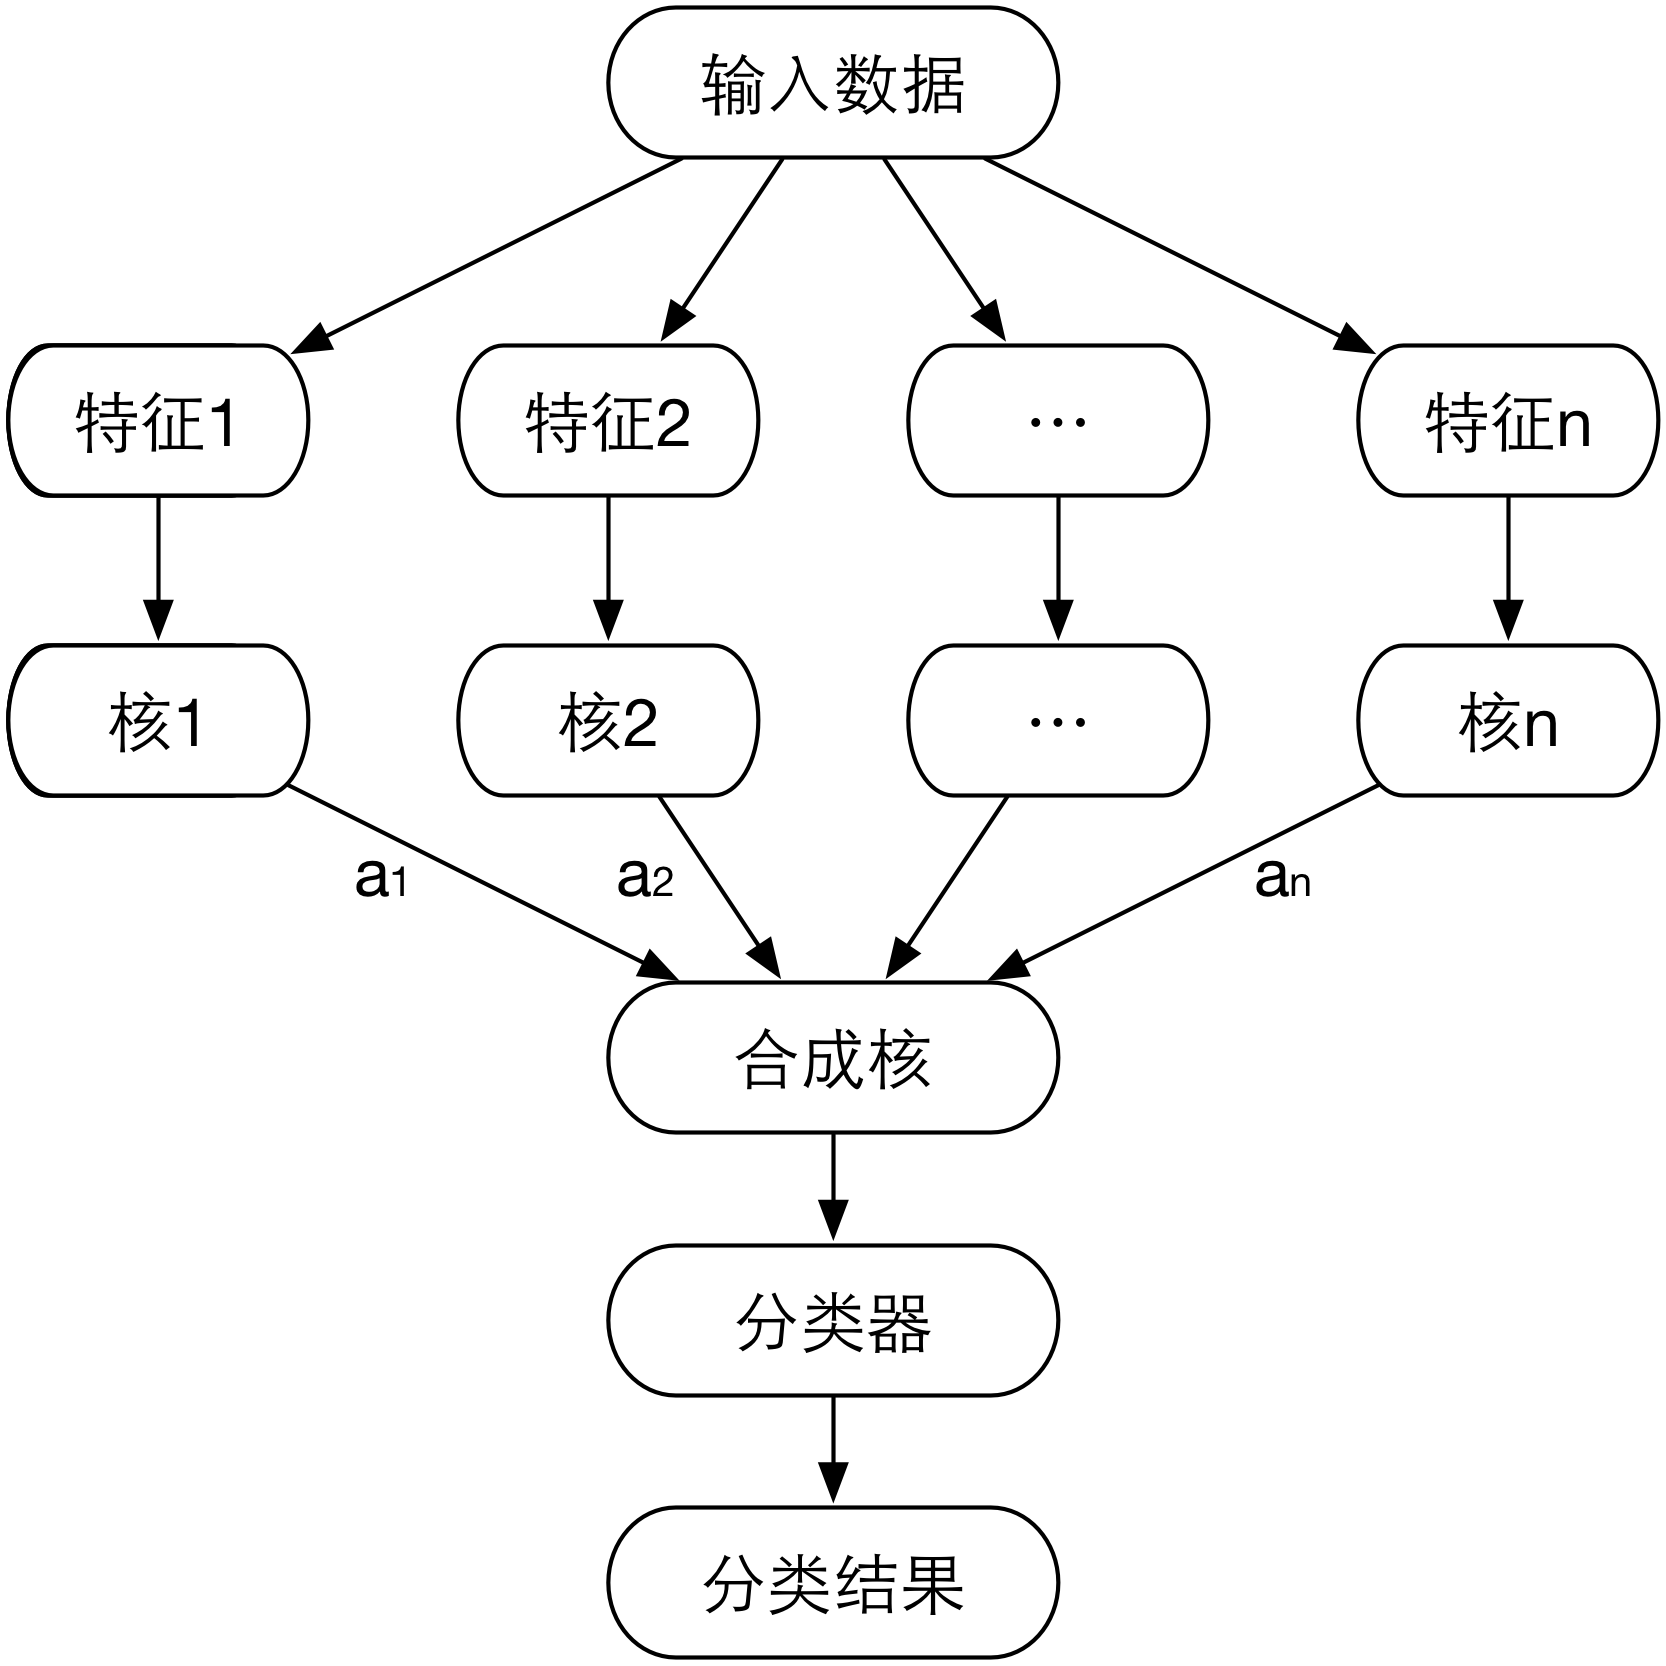
\includegraphics[height=7cm]{MKL/MKL}
  \caption{多核学习算法结构}
  \label{fig:MKL}
\end{figure}


% 确定上述判别函数通过解以下二次优化问题实现:
% \begin{eqnarray}
% \left\{ \begin{array}{l} \min \frac{1}{2}||w||^{2}_{2}+C\sum^{N}_{i=1}\xi_{i}\\
% w \in R^{s}, \xi \in R^{N}_{+}, b \in R\\
% y_{i}(<w,\phi(x_{i})>+b) \ge 1-\xi_{i} ~~~ \forall i \end{array} \right.
% \end{eqnarray}
% 其中,$w$是向量的权重,$C$为惩罚因子,$\xi$为松弛变量,$b$为超平面的偏置项。以上最优化问题并不是直接解,而是通过拉格朗日变换转化为对偶问题:
% \begin{eqnarray}
% \left\{ \begin{array}{l} \max\sum^{n}_{i=1}\alpha_{i}-\frac{1}{2}\sum^{n}_{i,j=1}\alpha_{i}\alpha_{j}y_{i}y_{j}\underbrace{< \phi(x_{i}),\phi(x_{j}) >}_{k(x_{i},x_{j})}\\
% \alpha \in R^{N}_{+}\\
% \sum^{N}_{i=1}\alpha_{i}y_{i}=0\\
% C \ge \alpha_{i} \ge 0 ~~~ \forall i\end{array} \right.
% \end{eqnarray}
% 上式中$k$为核函数。将上式代入到判别函数中可以得到:
% \begin{eqnarray}
% f(x)=\sum^{N}_{i=1}\alpha_{i}y_{i}k(x,x_{i})+b
% \end{eqnarray}



多核学习有六个关键属性:(1)确定结合函数的方法,(2)结合核函数的形式,(3)确定结合函数参数的目标函数形式,(4)计算结合函数参数的训练方法,(5)基本学习算法,(6)多核学习的计算复杂度。根据上述不同属性可以将多核学习算法进行分类~\cite{gonen2011multiple}:
\begin{enumerate}
\item 现有的多核学习算法用不同的学习方法来确定核结合函数的形式,根据方法的不同可以将这些算法分为5类:固定形式结合方法、启发式方法、最优化方法、贝叶斯方法和Boosting方法。
  \begin{itemize}
  \item 固定形式是指结合函数中没有任何参数,不需要训练,例如将核以固定的形式相加或相乘。
  \item 启发式方法采用有参数的结合函数组合基本核,根据核矩阵或每个核单独使用时的表现来确定函数的参数。
  \item 最优化方法也是使用有参数的结合函数,通过解最优化问题来确定参数。
  \item 贝叶斯方法将核结合函数的参数看做随机值,先设定这些参数先验值,然后通过推理学习参数。
  \item Boosting方法的思想来源于集成学习,通过迭代增加新的核直到分类性能不再提高为止。
  \end{itemize}
\item 多核学习算法根据核函数融合方式不同可以将其分为:线性结合、非线性结合和数据依赖结合。
  \begin{itemize}
  \item 线性结合是目前应用较广的方法,主要包括无权重求和和有权重求和两种。
  \item 非线性结合方法是指使用非线性函数做为结合函数,例如包含相乘、幂运算的函数。
  \item 数据依赖结合是指定特定的核权重给每组数据,学习每个区域中最优核结合方式。
  \end{itemize}
\item 确定结合函数参数能够根据优化不同目标函数得到,现有的目标函数一般分为三类:相似性函数、结构风险函数和贝叶斯函数。
  \begin{itemize}
  \item 相似性目标函数是通过最大化相似度来确定结合函数的参数(相似度是根据训练集计算出结合核矩阵和最优核矩阵之间的相似性)。
  \item 结构风险函数根据最小化正则项和误差项之和来确定结合函数的参数,这称之为结构风险最小化。
  \item 贝叶斯函数是用贝叶斯公式计算结合核的参数。
  \end{itemize}
\item 计算结合函数参数的训练方法包括两种。一种是直接计算出结合函数参数和基础核函数参数;另一种是通过迭代的方法实现,先固定基础核函数的参数,更新结合函数的参数,然后再固定结合函数的参数,更新基础核函数的参数,直到最终收敛就完成了训练。
\item 多核学习的基础学习算法有很多,例如支持向量机、核Fisher判别分析、核岭回归等。
\item 多核学习的计算复杂度主要依赖于训练方法和基础学习方法的复杂度。
\end{enumerate}

同支持向量机这样的单核学习算法相比,多核学习在训练中不仅要计算w,b的值,还要得到每个核函数的权重。在这里最重要的问题是如何确定权重,近年来许多多核学习算法都是针对这一问题提出的。

多核学习算法中最经典的方法是简单多核学习(SimpleMKL)~\cite{rakotomamonjy2008simplemkl},它被看做为多核学习算法的具体实现。后来人们还提出了广义多核学习(Generalized Multiple Kernel Learning, GMKL)~\cite{varma2009more}、局部多核学习(Localized Multiple Kernel Learning, LMKL)~\cite{gonen2008localized}、非线性多核学习(Non-Linear Multiple Kernel Learning, NLMKL)~\cite{cortes2009learning}等算法,下面对简单多核学习和本文中使用的非线性多核学习算法进行介绍。

\subsubsection{简单多核学习}
SimpleMKL~\cite{rakotomamonjy2008simplemkl}使用线性结合的方式将多个基础核函数组合得到一个新的核函数,并采用梯度下降法求解,其核函数形式为:
\begin{eqnarray}
K(x_{i},x_{j})=\sum^{M}_{m=1}d_{m}k_{m}(x_{i},x_{j}), ~~~ with ~ d_{m} \ge 0, ~\sum^{M}_{m=1}d_{m}=1
\end{eqnarray}
上式中,$k_{m}$表示基础核函数,$M$表示基础核函数的数量,$d_{m}$是基础核函数对应的权重系数,它表示着特征在分类过程中的重要性,是多核学习过程中需要求解的重要问题。根据支持向量机的原理,SimpleMKL的原始优化问题可以等价为如下凸优化问题~\cite{孙锐2014基于多特征和多核学习的行人检测方法的研究}:
\begin{eqnarray}
\left\{ \begin{array}{l} \min \frac{1}{2}\sum_{m}\frac{1}{d_{m}}||f_{m}||^{2}+C\sum_{i}\xi_{i}\\
s.t ~~~ y_{i}\sum^{M}_{m=1}f_{m}(x_{i})+y_{i}b \ge 1-\xi ~~~ \forall i\\
\xi_{i}\ge 0 ~~~ \forall i\\
\sum^{M}_{m=1}d_{m}=1, ~~~ d_{m} \ge 0 ~~ \forall m\end{array} \right.
\end{eqnarray}
上式中,$f_{m}$为希尔伯特空间中的分类超平面。该式为多核学习的原始问题,要根据其确定参数$d_{m}$。采用拉格朗日算法可以将上述原始优化问题转换成对偶问题得到:
\begin{multline}
L=\frac{1}{2}\sum_{m}\frac{1}{d_{m}}||f_{m}||^{2}+C\sum_{i}\xi_{i}+\sum_{i}\alpha_{i}(1-\xi_{i}-y_{i}\sum_{m}f_{m}(x_{i})-y_{i}b)\\
-\sum_{i}v_{i}\xi_{i}+\lambda(\sum_{m}d_{m}-1)-\sum_{m}\eta_{m}d_{m}
\end{multline}
其中$\alpha_{i}$和$v_{i}$为拉格朗日乘子,而$\lambda$和$\eta_{m}$表示权重$d_{m}$的约束。接着分别对$L$自变量求偏导数,并令导数为0可得:%$f_{m},b,\xi_{m},d_{m}$
\begin{eqnarray}
\left\{ \begin{array}{l}\frac{1}{d_{m}}f_{m}(\bullet)=\sum_{i}\alpha_{i}y_{i}K_{m}(\bullet,x_{i}), ~~~ \forall m\\
\sum_{i}\alpha_{i}y_{i}=0\\
C-\alpha_{i}-v_{i}=0, ~~~ \forall i\\
-\frac{1}{2}\frac{||f_{m}||^{2}}{d^{2}_{m}}+\lambda-\eta_{m}=0, ~~~ \forall m\end{array} \right.
\end{eqnarray}

采用拉格朗日得到的对偶问题由于持续约束难以优化,这种约束可能转移到目标函数,但是目标函数变为不可微的,同样会造成求解困难。SimpleMKL带约束的优化问题为:
\begin{eqnarray}
\min_{d}J(d) ~~ s.t. \sum^{M}_{m=1}d_{m}=1,d_{M}\ge 0\\
J(d)=\left\{\begin{array}{l}\min_{{f},b,\xi}\frac{1}{2}\sum_{m}\frac{1}{d_{m}}||f_{m}||^{2}+C\sum_{i}\xi_{i} ~~~ \forall i\\
s.t. ~~~ y_{i}\sum_{m}f_{m}(x_{i})+y_{i}b \ge 1-\xi_{i}\\
\xi_{i}\ge 0 ~~~ \forall i\end{array}\right.
\end{eqnarray}

将上式可以转化为对偶问题:
\begin{eqnarray}
J(d)=-\frac{1}{2}\sum_{i,j}\alpha_{i}\alpha_{j}y_{i}y_{j}\sum{m}d_{m}K_{m}(x_{i},x_{j})+\sum_{i}\alpha_{i}
\end{eqnarray}

采用梯度下降法计算$J(d)$的梯度下降表示,不断的更新$d$的值直到满足停止准则。根据支持向量机求解原理,SimpleMKL的决策函数为:
\begin{eqnarray}
f(x)=s(\sum^{N}_{i=1}\sum^{M}_{m=1}d_{m}\alpha_{i}y_{i}K_{m}(x_{i},x_{j})+b)
\end{eqnarray}

\subsubsection{非线性多核学习}

上面介绍的简单多核学习得到的分类器性能要比使用单个核的支持向量机好,该方法实质上可以看成支持向量机使用多个不同核函数的线性组合。Gonen等人在2011发表的文章~\cite{gonen2011multiple}中对多种多核学习算法的性能进行了分析,他们在多个数据集上进行实验发现,采用非线性多核学习更有利于改善分类的性能。本文设计的浮游生物分类系统正是使用了非线性多核学习进行特征融合和训练分类器。Cortes等人~\cite{cortes2009learning}提出了非线性多核学习(Non-linear Multiple Kernel learning, NLMKL),该方法基于核岭回归(Kernel ridge regression, KRR)采用多项式函数将核进行融合,他们提出的结合核的形式如下:
\begin{eqnarray}
K_{\eta}(x_{i},x_{j})=\sum_{q\in Q}\eta_{q_{1}q_{2}\cdots q_{m}}k_{1}\cdots k_{m}
\end{eqnarray}
其中$Q=\{q:q\in Z^{m}_{+}, \sum^{m}_{l=1}q_{l}\le d\}$。然而上式中需要学习的参数较多,为了减少学习的复杂度,将其化简为:
\begin{eqnarray}
K_{\eta}(x_{i},x_{j})=\sum_{q\in R}\eta^{q_{1}}_{1}\eta^{q_{2}}_{2}\cdots\eta^{q_{m}}_{m}k_{1}\cdots k_{m}
\end{eqnarray}
其中$R=\{q:q\in Z^{m}_{+}, \sum^{m}_{l=1}q_{l}=d\}$。例如,当$d=2$时,核函数为:
\begin{eqnarray}
K_{\eta}(x_{i},x_{j})=\sum^{m}_{l=1}\sum^{m}_{h=1}\eta_{l}\eta_{h}k_{l}k_{h}
\end{eqnarray}

在该非线性多核学习中,结合核函数的权重通过解最小-最大优化问题来求得。\\


在浮游生物的分类识别过程中为了提高分类的准确度通常要融合多种特征。在遇到多种特征进行分类的问题时,只采用单个核函数进行分类并不能充分发挥每种特征的作用。多核学习是通过为每种特征选择分别选择核函数并融合在一起来构建分类器,这种方法可以有效的处理特征并解决单一核函数存在的不足。本文中我们使用非线性多核学习~\cite{cortes2009learning}来设计浮游生物分类系统,下面该分类系统进行详细介绍。

\section{基于多核学习的浮游生物图像分类系统}
\label{sec:system}

我们研究浮游生物自动分类系统的出发点是扩大其适用范围,提高分类性能。因此在设计分类系统时采用多种特征提取方法对浮游生物形态特征进行描述,并结合了特征选择和多核学习方法来构建分类模型。本文提出的浮游生物自动分类系统由以下四个部分组成:图像预处理、特征提取、特征选择、多核学习,其算法结构流程图如图~\ref{fig:frame}所示。
\begin{figure}[H] % use float package if you want it here
  \centering
  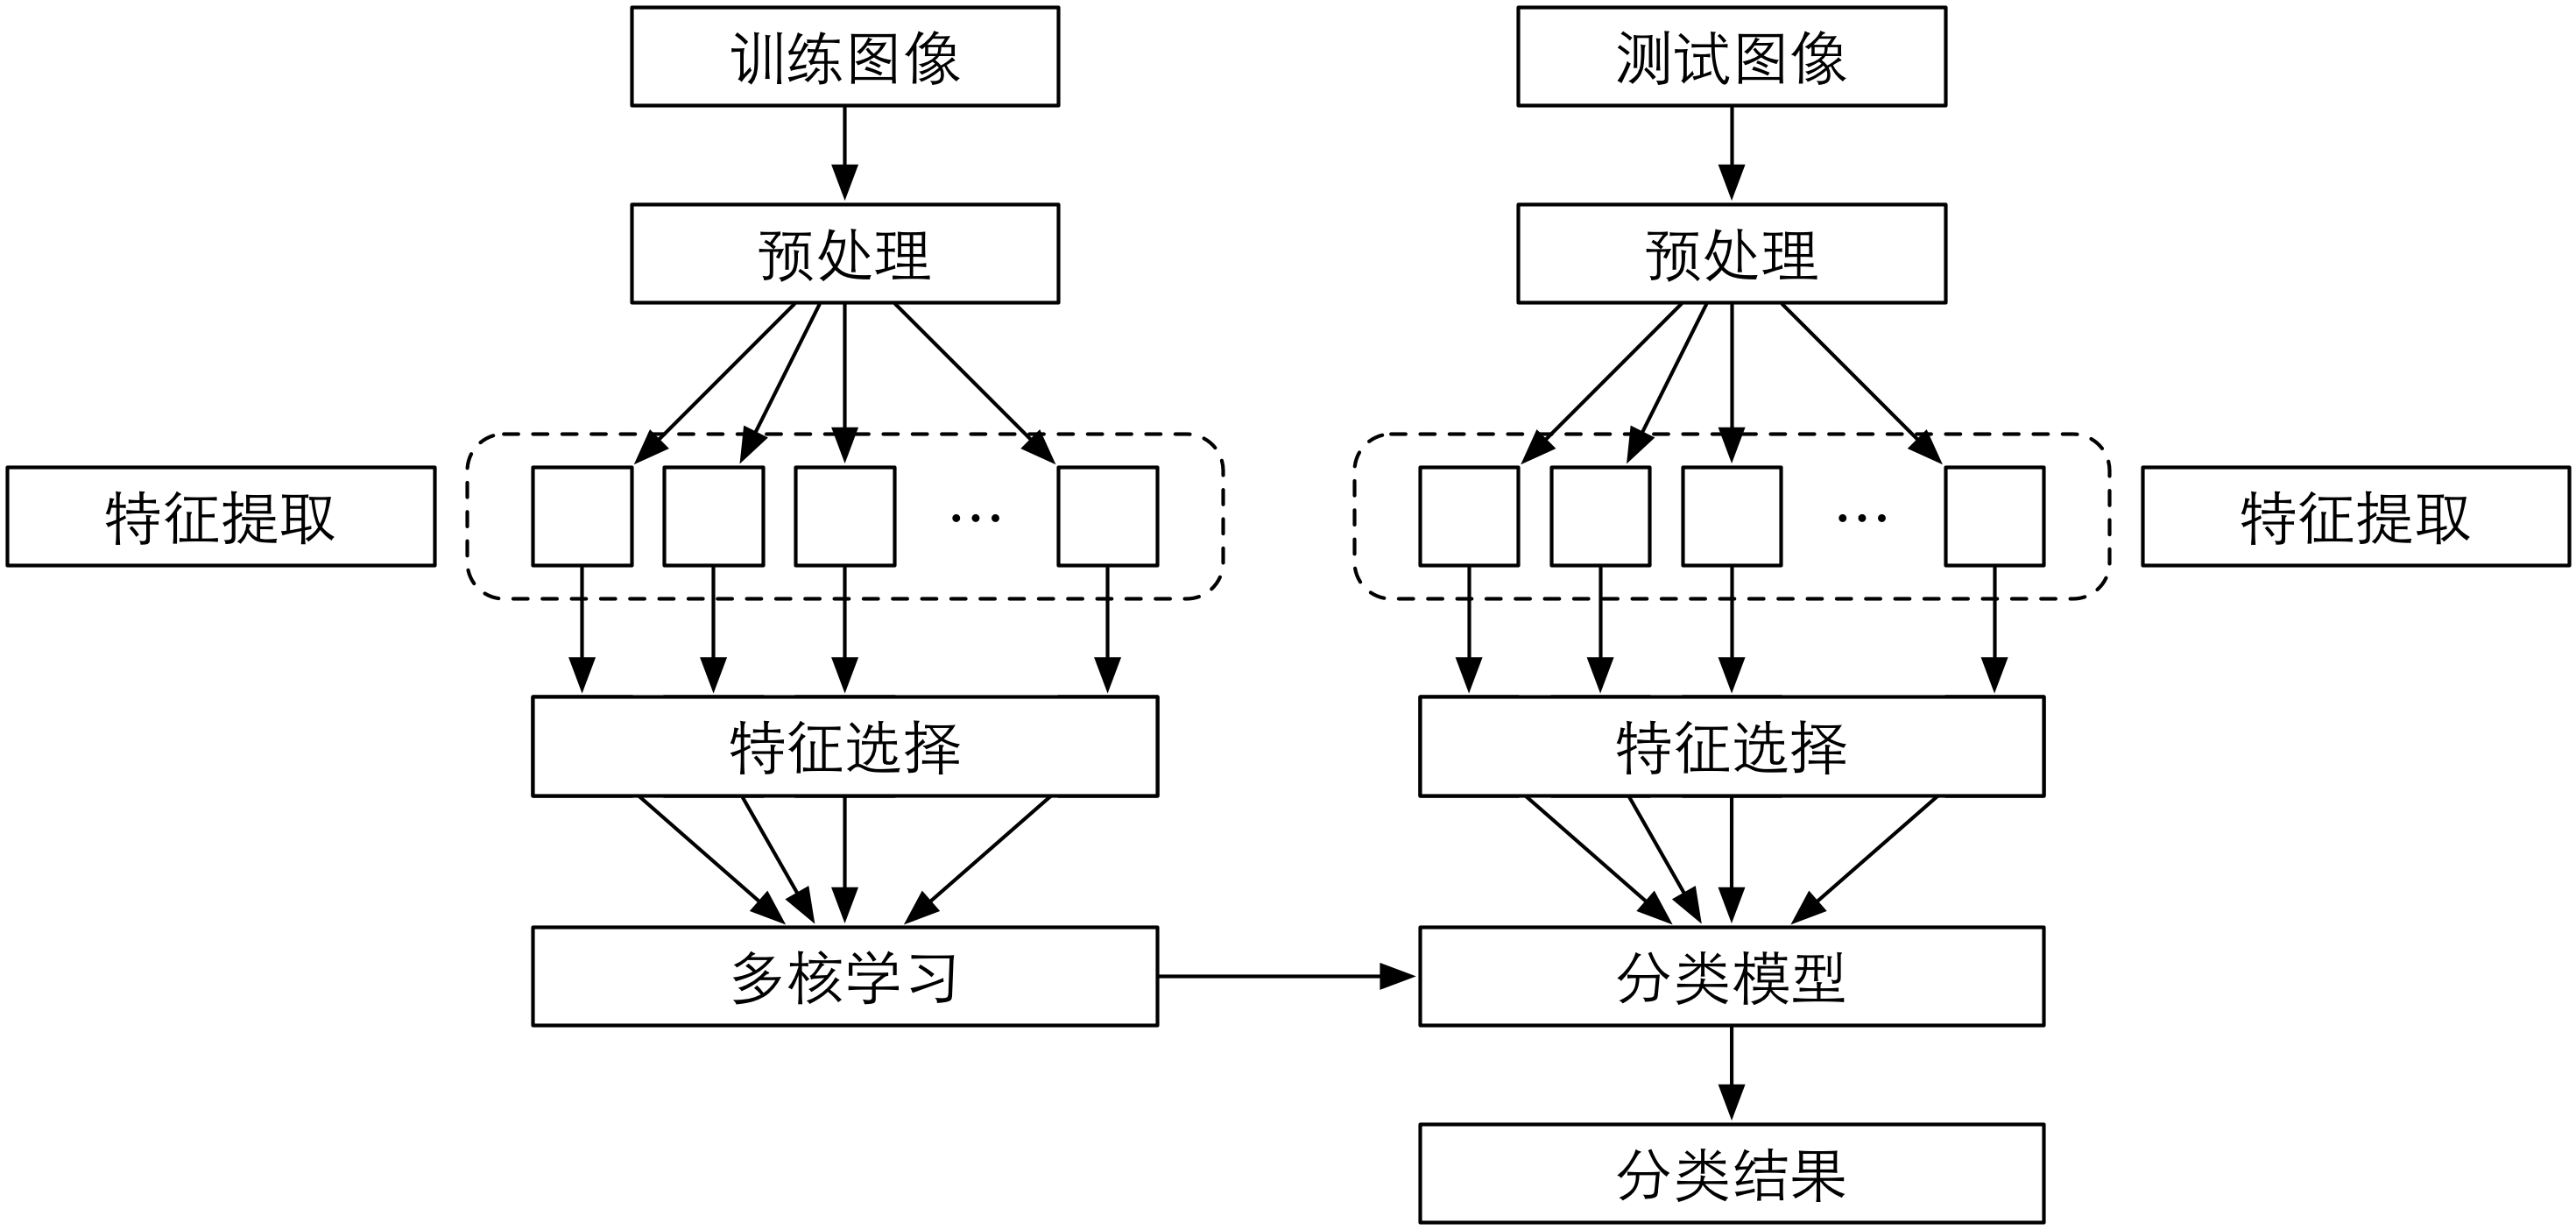
\includegraphics[height=6cm]{frame}
  \caption{基于多核学习的浮游生物分类系统算法结构流程图}
  \label{fig:frame}
\end{figure}

1、图像预处理

图像预处理是在图像识别之前进行的准备工作,包括去除图中的噪声、二值化分割图像背景等处理,避免无关因素对之后分类的影响。浮游生物数据集中的图像由水下图像采集设备获得,在采集浮游生物图像的过程中不可避免的会受到水中杂质等因素的干扰,造成采集的图像中会含悬浮物等噪声。因此为了提高图像的质量,在进行特征提取前要对采集的浮游生物图像进行预处理。

在本文实验使用的三个数据集中,WHOI采集的浮游生物图像没有分割,因此在预处理时首先要对该数据集进行分割。对该数据集的图像通过检测边缘进行分割~\cite{sosik2007automated}:首先将灰度图像进行相位一致性计算,然后采用Canny算子检测图像中的边缘,将获得的边缘图像用数学形态学算法(闭运算、膨胀、细化)进行处理,得到简单的轮廓边缘,使用获得的轮廓边缘就可以对其对应的浮游生物图像进行分割。

由于原浮游生物图像中可能存在悬浮颗粒等杂质,分割后图像中除了浮游生物外还会存在着小的杂质区域,因此在预处理过程中我们进行如下操作:首先得到原图像的二值图,然后采用数学形态学方法,去掉二值图像中面积小于一定像素数量的小连通区域;之后用得到的二值图对原图像重新做分割,获得去除噪声后的图像。图~\ref{fig:nonoise}中显示了预处理前后的浮游生物图像,能够看出图像~\ref{fig:nonoise4}中的杂质点明显减少。
\begin{figure}[h]
  \centering%
  \subcaptionbox{原图像\label{fig:nonoise1}}%标题的长度,超过则会换行,如下一个小图。
    {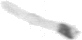
\includegraphics[height=2cm]{Preprocess/nonoise1}}%
  \hspace{2em}%
  \subcaptionbox{原图像的二值图\label{fig:nonoise2}}
      {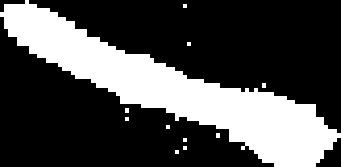
\includegraphics[height=2cm]{Preprocess/nonoise2}}\\
      ~\newline
  %\hspace{2em}%
  \subcaptionbox{预处理后的二值图\label{fig:nonoise3}}
      {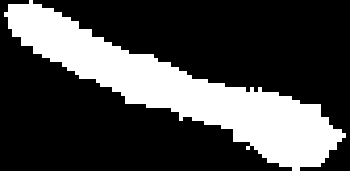
\includegraphics[height=2cm]{Preprocess/nonoise3}}
  \hspace{2em}%
  \subcaptionbox{预处理后的图像\label{fig:nonoise4}}
      {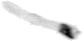
\includegraphics[height=2cm]{Preprocess/nonoise4}}
  \caption{图像预处理}
  \label{fig:nonoise}
\end{figure}

2、特征提取

采用~\ref{sec:FeatureExtraction}章节中提到特征描述方法对浮游生物的形态特征进行提取,可以实现从纹理、形状、灰度等不同角度对浮游生物形态特征进行描述。在特征提取后可以将提取的特征分为10类(每种特征提取方法提取的特征作为一类,其中粒子测度采用两组参数可以得到两组特征,将这两组特征分别作为一类),如图~\ref{fig:framework}所示。

3、特征选择

 在上一步中从不同角度提取了丰富的特征对浮游生物进行描述,然而这些特征中可能存在冗余或不相关的部分,它们不仅对分类性能的提高没有积极作用,甚至还会影响分类效率。因此,使用特征选择从所有特征中选取最优子集、去除冗余部分,可以提高分类的性能和效率。并且,对不同数据集进行分类时,采用特征选择可以针对每一个数据集从所有特征中找到适合的特征组合。本文采用了基于封装式评价准则的特征选择方法~\cite{Kohavi1997Wrappers},针对特征提取部分获得的10类特征分别进行选择,如图~\ref{fig:framework}所示。

4、多核学习

针对特征提取和特征选择后得到的10组特征信息,为每组特征分别选定3种核函数,采用多核学习的方法通过融合核函数实现特征的融合。在本文中使用非线性多核学~\cite{cortes2009learning}将所有核函数融合到一起,同时训练得到最终分类器,如图~\ref{fig:framework}所示。最终得到的分类器可以对未知的浮游生物图像进行识别,并具有广泛的适用范围和较高的准确率。下面设计对比实验对分类系统的性能进行评价。

\begin{figure}[H] % use float package if you want it here
  \centering
  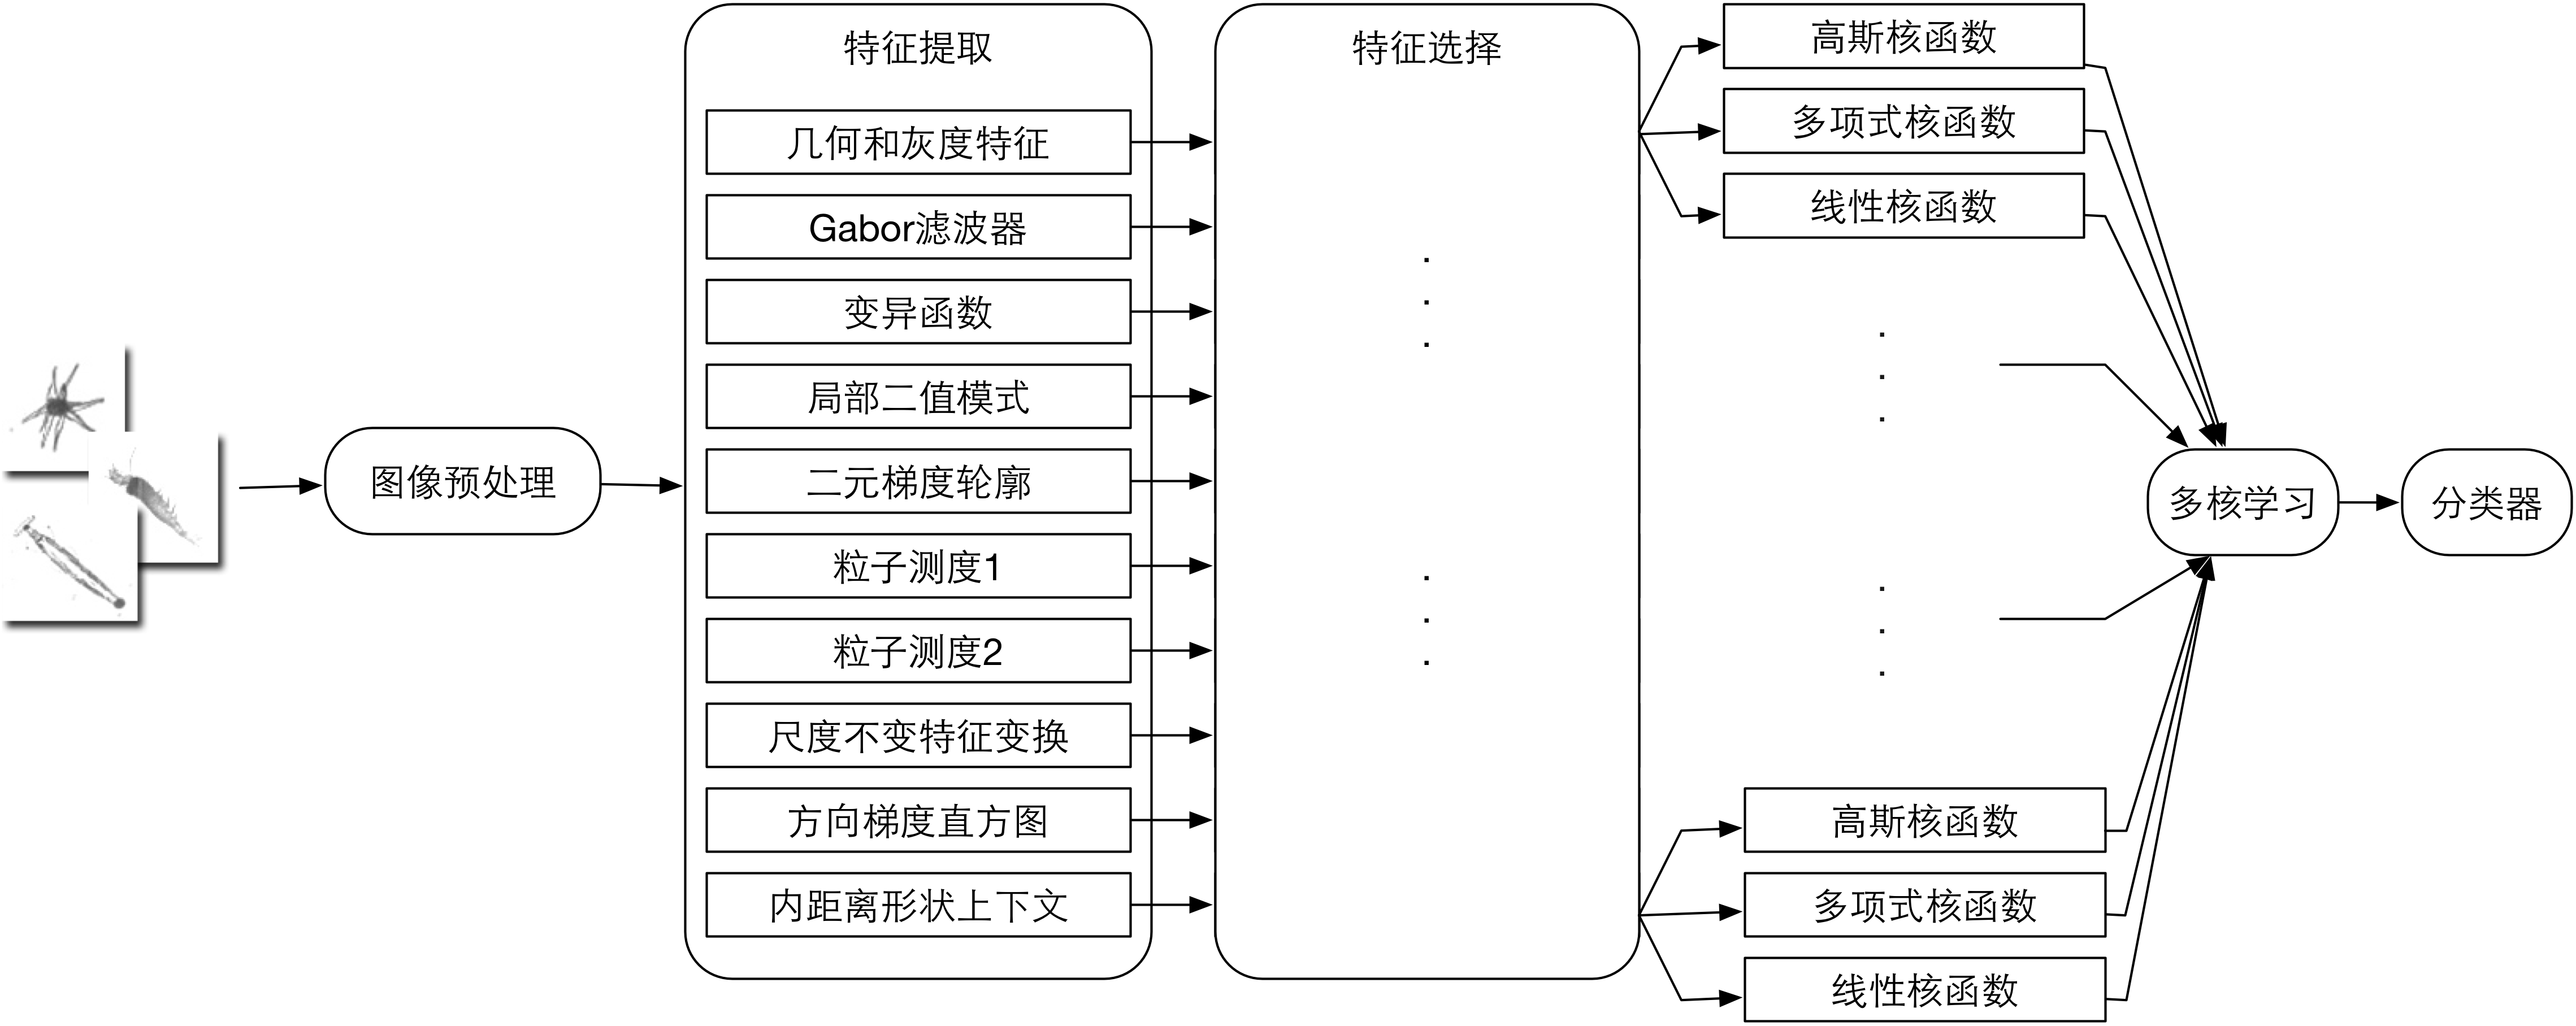
\includegraphics[height=6cm]{frame/framework}
  \caption{基于多核学习的浮游生物分类系统详细算法流程}
  \label{fig:framework}
\end{figure}

\section{对比实验}
\label{sec:experiment}

为了对本文设计的浮游生物分类系统的性能进行分析和评价,我们设计了如下三组对比实验:实验一是结合目前分类性能较好的浮游生物分类方法设计一个基准分类系统,作为分类系统性能对比评价的基准;实验二是在实验一的基础上,将使用~\ref{sec:FeatureExtraction}中提到的特征提取方法来对浮游生物特征进行描述;实验三采用本文设计的基于多核学习的浮游生物分类系统进行实验。将以上三个实验进行对比分析,从而实现对浮游生物分类系统各部分性能的评价。

\subsection{基准实验}
\label{sec:baselineExperiment}

根据Sosik等人在2007年提出的浮游植物自动分类方法~\cite{sosik2007automated}和ZooScan系统~\cite{gorsky2010digital}设计浮游生物分类的基准系统,该基准系统的算法流程框图如图\ref{fig:shiyan1frame}所示。
\begin{figure}[H] % use float package if you want it here
  \centering
  
\includegraphics[height=0.7cm]{shiyan/shiyan1/shiyan1}
  \caption{基准实验的算法流程框图}
  \label{fig:shiyan1frame}
\end{figure}

首先对浮游生物图像进行预处理,降低图像中的噪声信息。然后对浮游生物形态特征进行提取,这里使用的特征提取方法结合了Sosik论文中的210个特征和ZooScan系统中的53个特征,因此经过特征提取每幅图像可以获得一个263维的特征向量。在得到每幅图像的特征后,采用特征选择除去其中的冗余部分。经过特征选择后,三个数据集保留下来的特征维数如表~\ref{tab:weishu}所示。最后对保留的特征归一化,用支持向量机算法来训练分类器,并使用混淆矩阵统计实验结果和分类准确率。

\begin{table}[htbp]
\small
  \centering
  \caption{特征选择后得到的特征维数}
  \label{tab:weishu}
  \begin{tabular}[c]{cccc}
    \toprule
    %\hline
    ~ & WHOI数据集 & ZooScan数据集 & Kaggle数据集\\
    \midrule
    %\hline
    特征维数 & 90 & 88 & 100\\
    \bottomrule
    %\hline
  \end{tabular}
\end{table}

该实验在~\ref{sec:dataset}中介绍的三个数据集上得到结果如表~\ref{tab:shiyan1Result}所示,混淆矩阵如图~\ref{fig:shiyan1}(图中横轴和纵轴为数据集中浮游生物的种类,见附录~\ref{fulu};图中数值表示分为对应类别图像的数量,数值越大颜色越深)。在WHOI采集的数据集上分类结果的F-Measure为0.8832,比相同条件下Sosik论文~\cite{sosik2007automated}中的分类结果有所提高。在ZooScan系统采集的数据集上得到分类结果的F-Measure为0.8212,相比于ZooScan系统的分类结果(0.7947)~\cite{gorsky2010digital}有一定提高。由此可以看出该实验设计的基准分类方法有较好的分类性能,可以作为评价浮游生物分类性能的基准。

\begin{figure}[h]
  \centering%
  \subcaptionbox{WHOI采集的数据集\label{fig:shiyan1whoiCM}}%标题的长度,超过则会换行,如下一个小图。
    {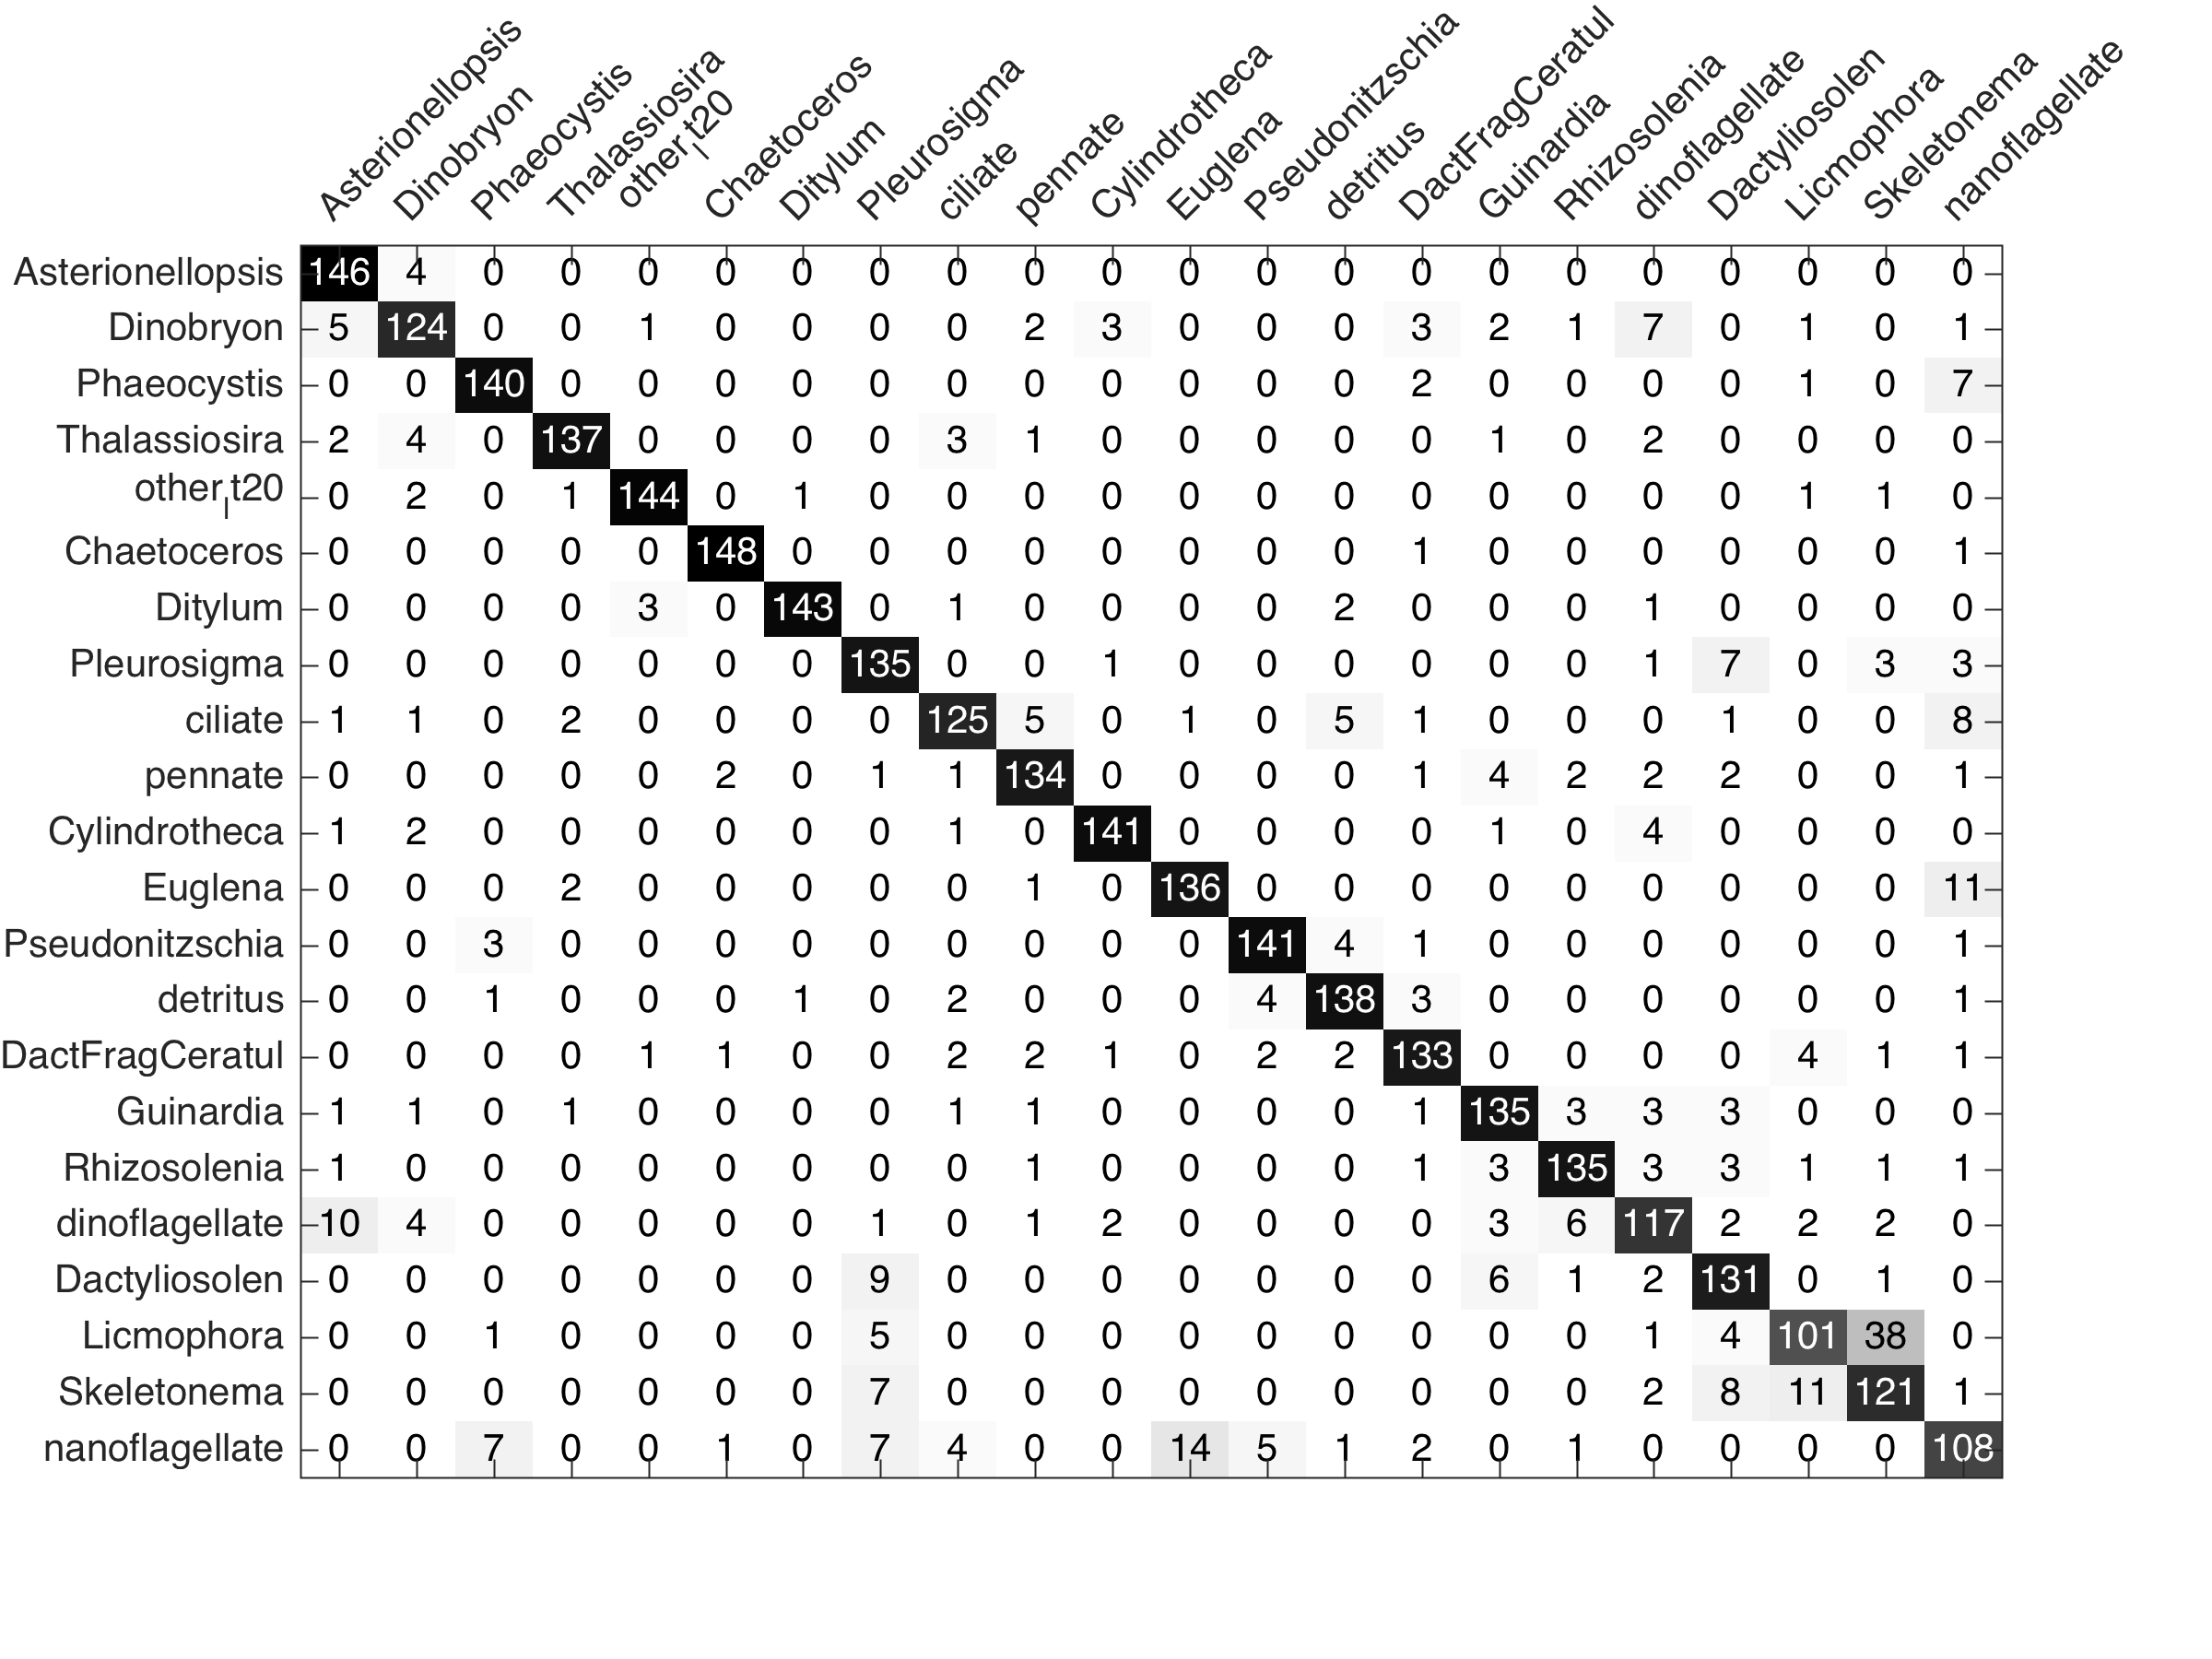
\includegraphics[height=5.5cm]{shiyan/shiyan1/whoiCM}}%\\%
  %~\newline
  %\hspace{2em}%
  \subcaptionbox{ZooScan采集的数据集\label{fig:shiyan1zooscanCM}}
      {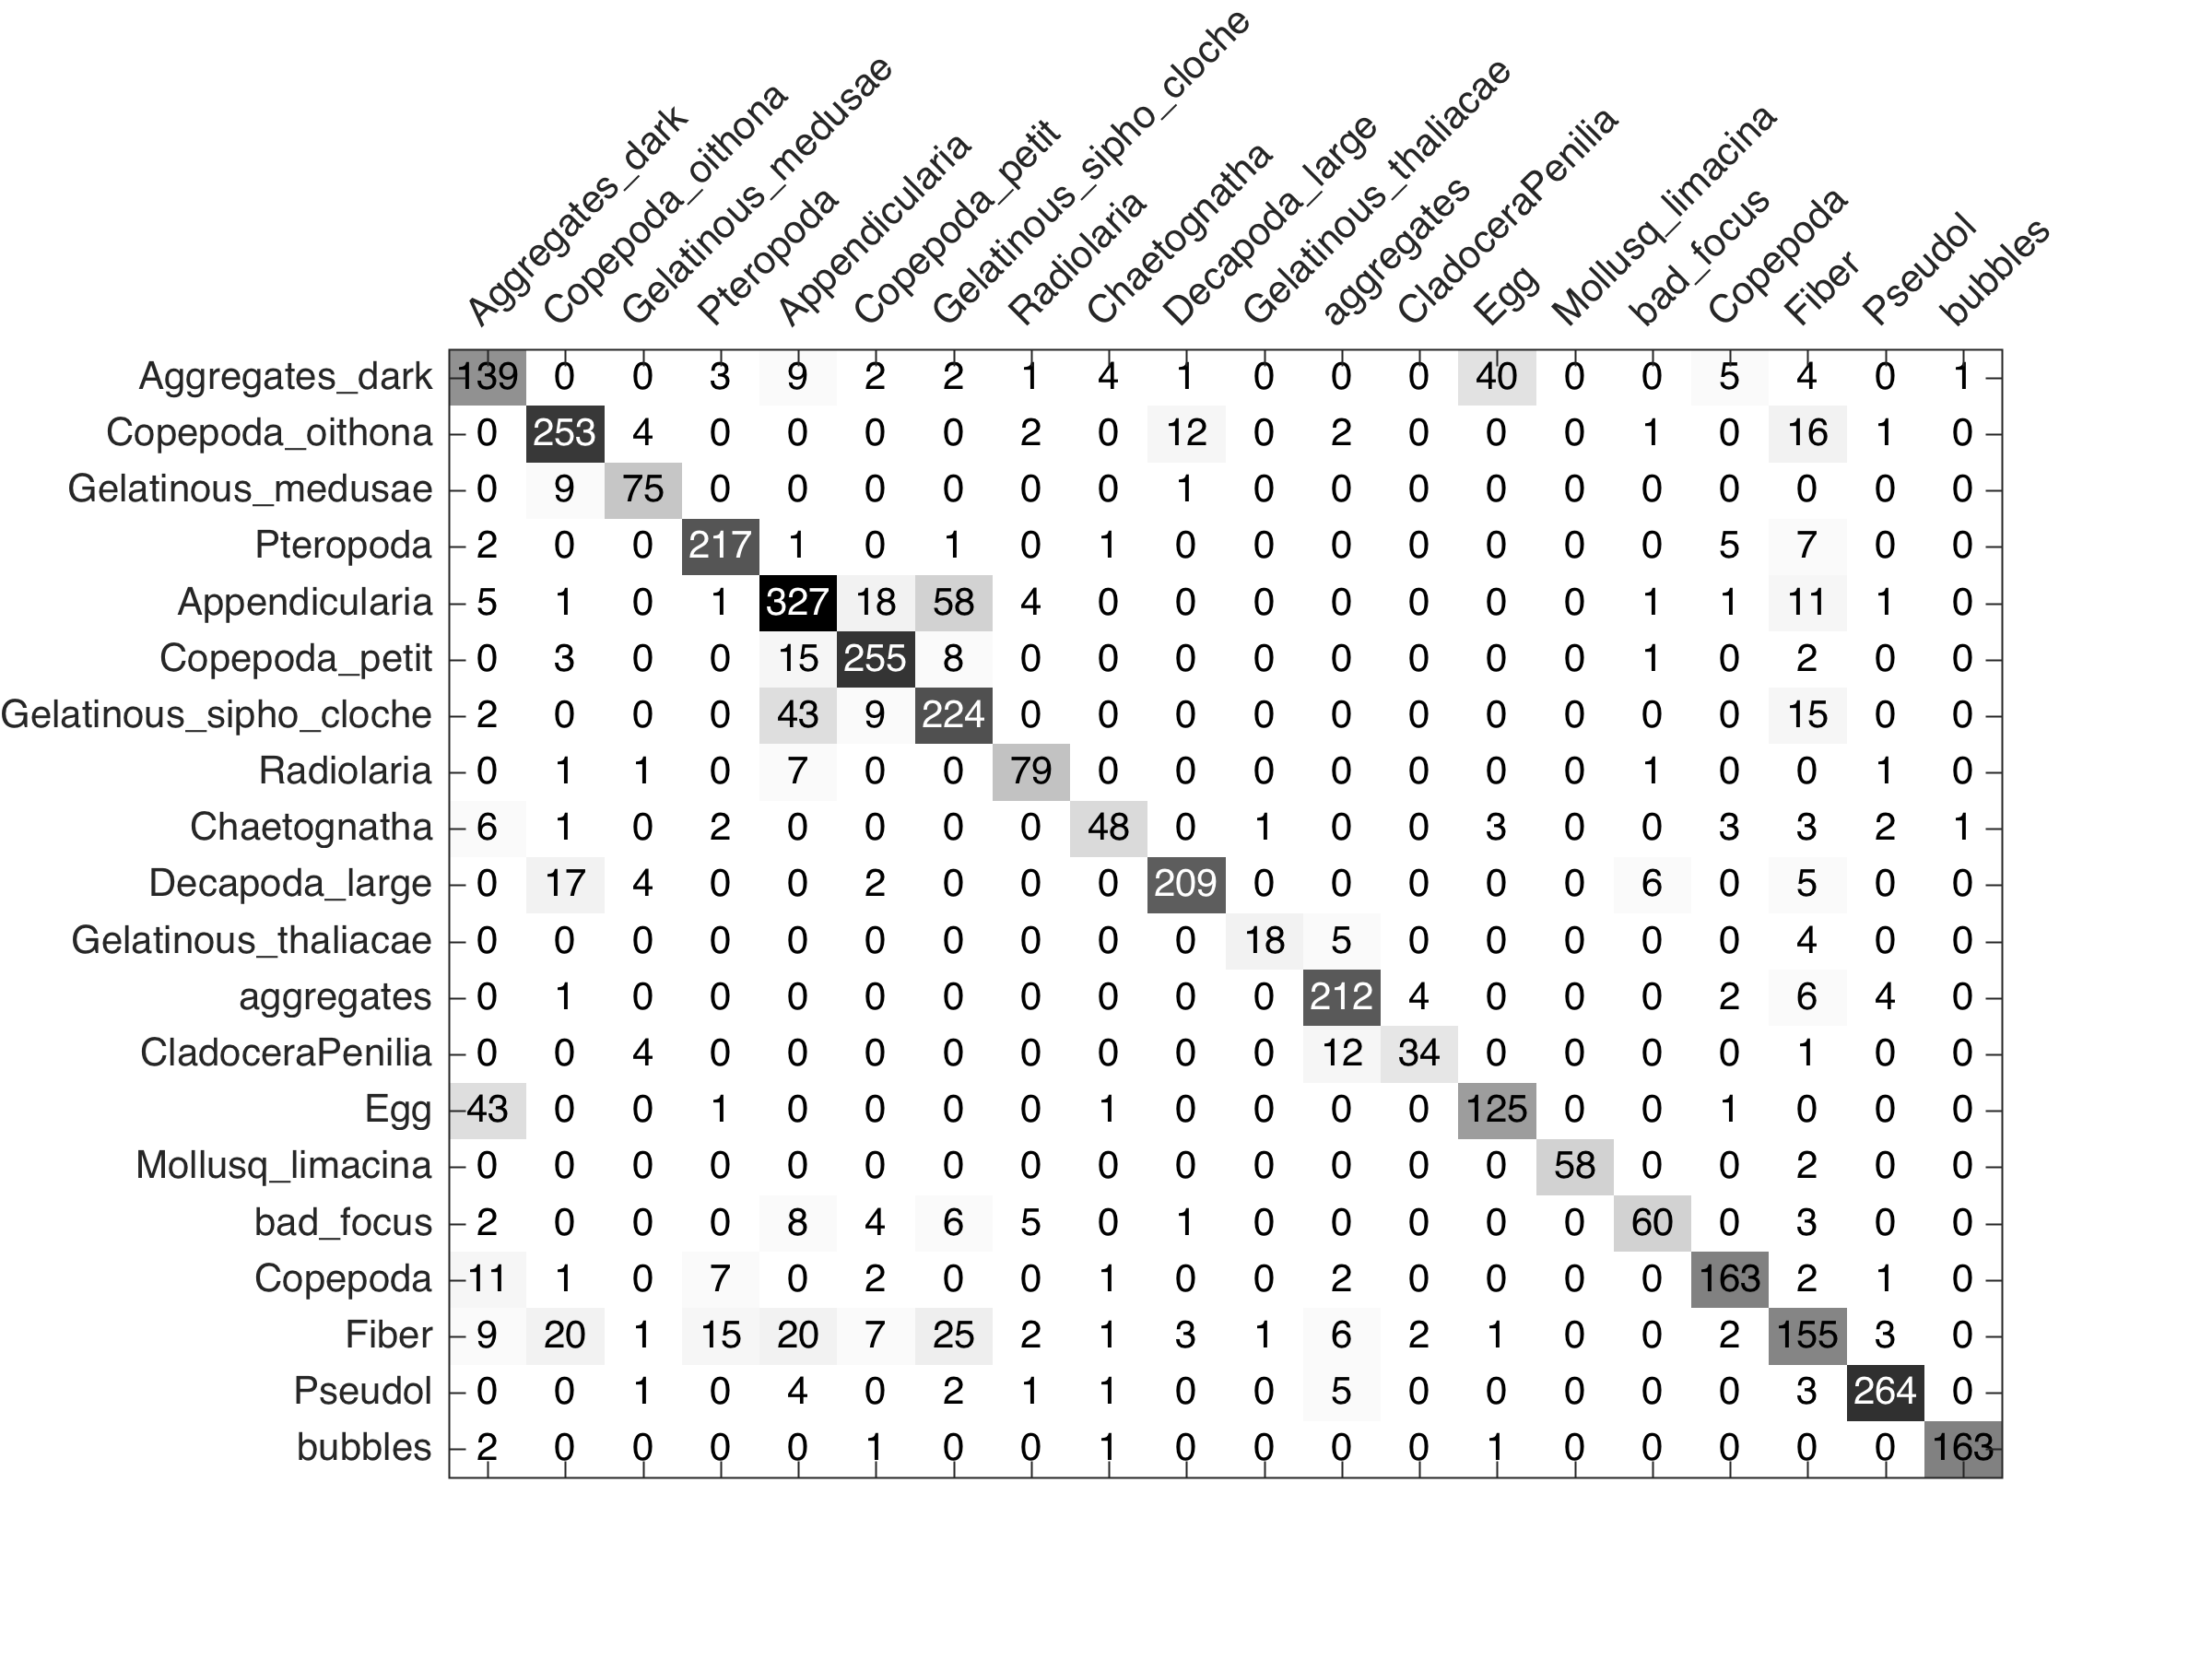
\includegraphics[height=6cm]{shiyan/shiyan1/zooscanCM}}\\
  ~\newline
  %\hspace{2em}%
  \subcaptionbox{Kaggle竞赛数据集\label{fig:shiyan1kaggleCM}}
      {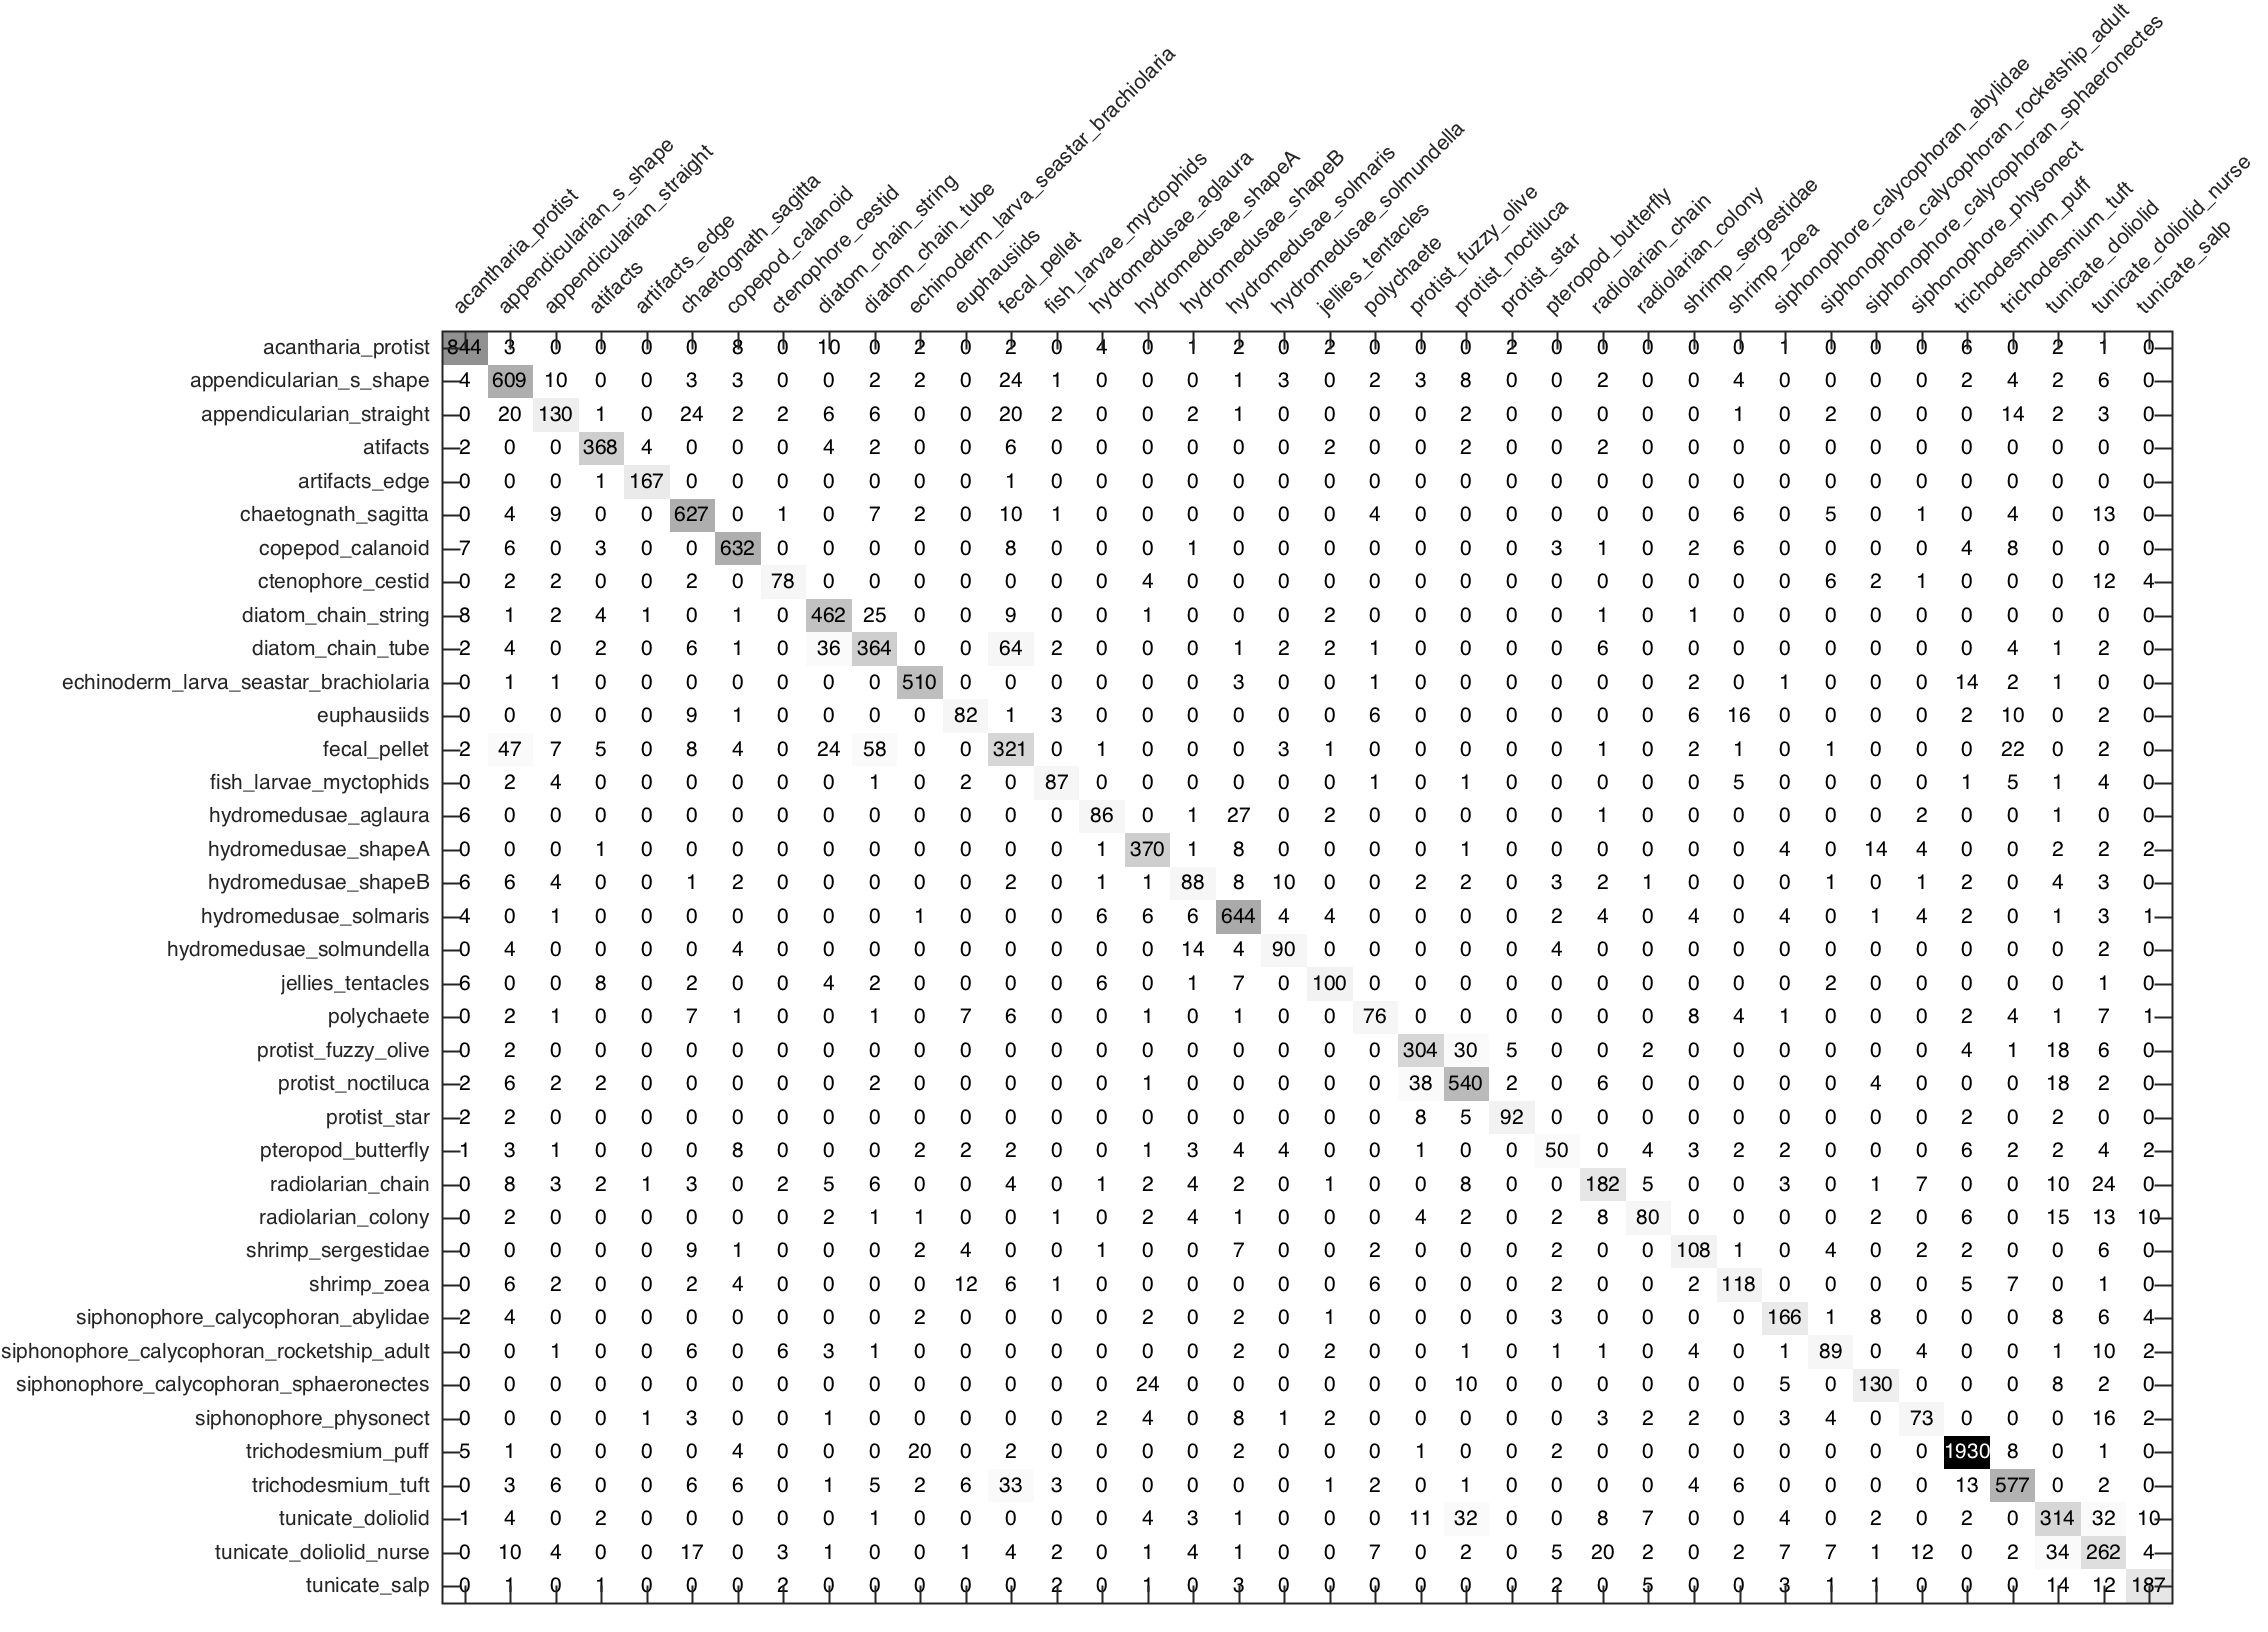
\includegraphics[height=11cm]{shiyan/shiyan1/kaggleCM}}
  \caption{基准实验分类结果的混淆矩阵}
  \label{fig:shiyan1}
\end{figure}

\begin{table}[htbp]
\small
  \centering
  \caption{基准实验的分类结果}
  \label{tab:shiyan1Result}
  \begin{tabular}[c]{cccc}
    \toprule
    %\hline
    ~ & WHOI数据集 & ZooScan数据集 & Kaggle数据集\\
    \midrule
    %\hline
    Recall & 0.8827 & 0.8060 & 0.7536\\
    %\hline
    %1-Precision & 11.63\% & 16.3\% & 21.49\%\\
    Precision & 0.8837 & 0.8370 & 0.7851\\
    F-Measure & 0.8832 & 0.8212 & 0.7690\\
    \bottomrule
    %\hline
  \end{tabular}
\end{table}

\subsection{特征对比实验}
\label{sec:featureexperiment}

在基准系统的基础上设计特征对比实验,使用~\ref{sec:FeatureExtraction}中的特征提取方法来对浮游生物进行描述,从而对本文设计分类系统的特征提取部分的性能进行评价,该实验的基本算法流程如图~\ref{fig:shiyan2frame}。
\begin{figure}[htbp] % use float package if you want it here
  \centering
  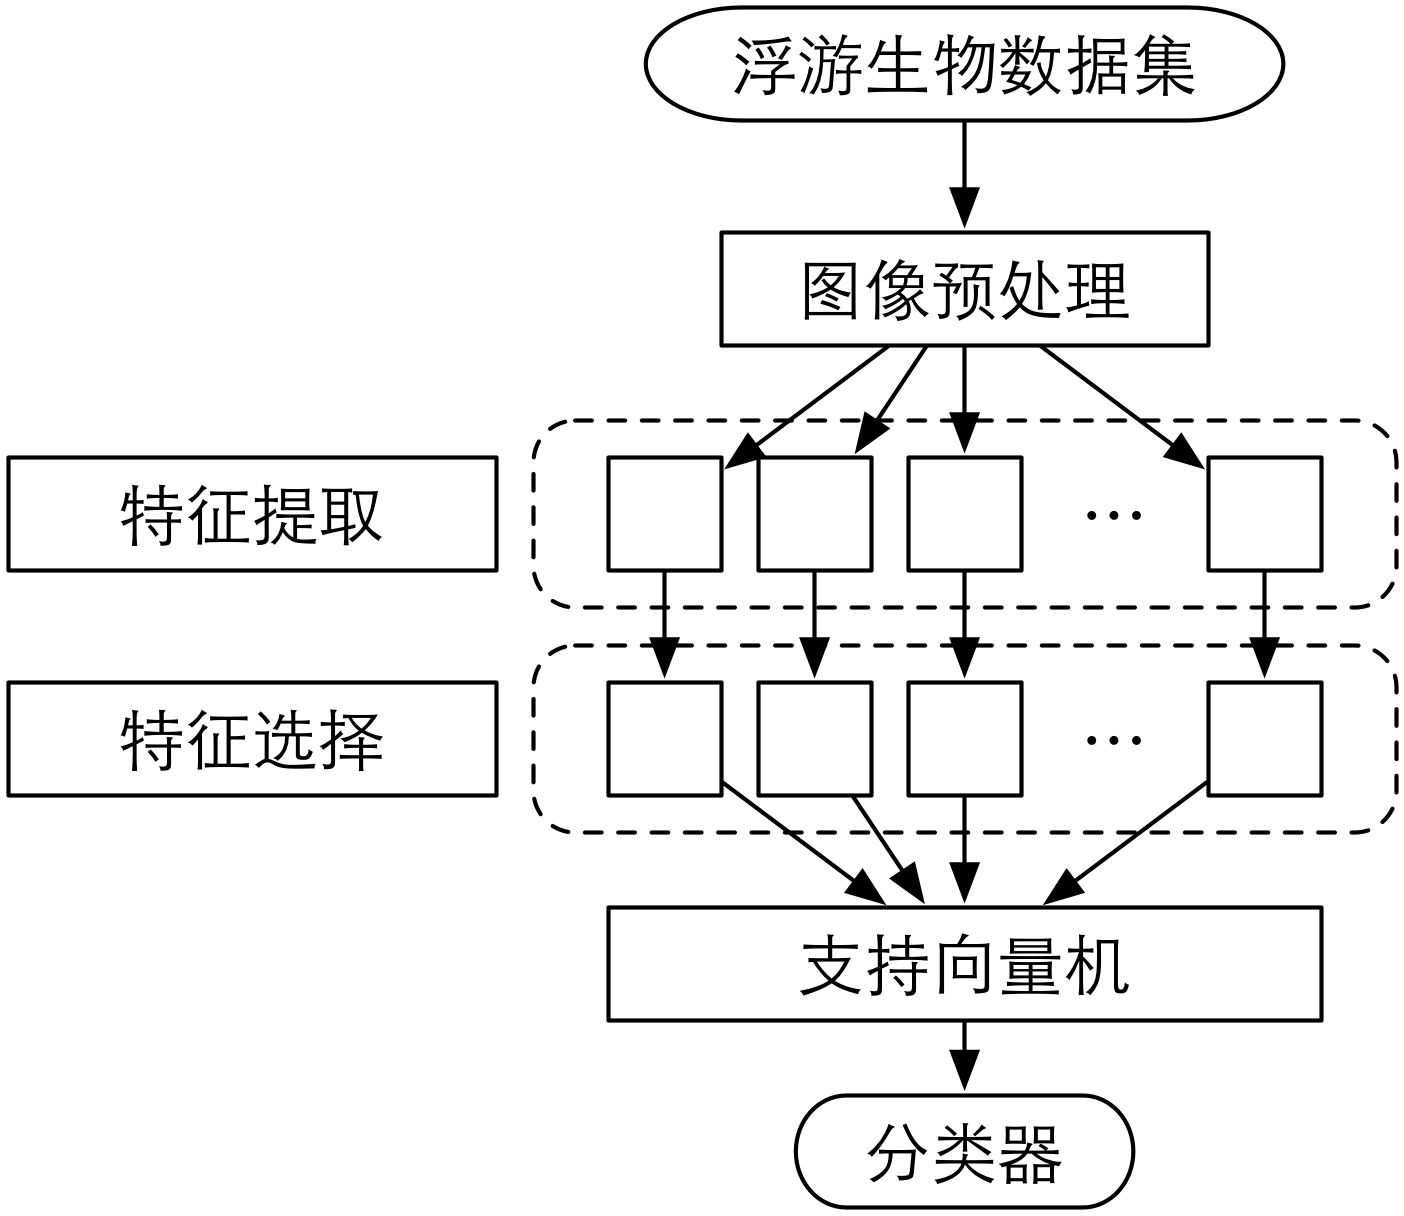
\includegraphics[height=6cm]{frame/jishu}
  \caption{特征对比实验算法流程框图}
  \label{fig:shiyan2frame}
\end{figure}

首先进行图像预处理,然后采用~\ref{sec:FeatureExtraction}中的特征提取方法分别提取浮游生物的形状、纹理等特征。在完成特征提取后,将所有特征分为10类(每类特征提取方法提取得到的特征作为一类,其中粒子测度采用两组参数提取特征得到两组特征)。针对每类特征分别采用特征选择方法去除冗余特征,然后将经过特征选择后的到的所有特征串联在一起,用支持向量机训练得到最终的分类器。

在三个数据集上进行实验时,支持向量机采用不同参数得到的分类结果如表~\ref{tab:shiyan2Result}所示。从表~\ref{tab:shiyan2Result}中能够得到,本实验在三个数据集上得到的最优分类结果及其相应的参数为:当采用高斯核函数且惩罚因子C=100时在WHOI取得最好分类结果,对应的F值为0.8963;在ZooScan系统采集的数据集上,当使用高斯核函数且C=10时取得最优分类结果,F值为0.8609;在Kaggle数据集上进行实验时采用高斯核函数且C=10取得最优分类结果,F值为0.8304。本实验在这三个数据集上取得的最优分类结果的混淆矩阵如图~\ref{fig:shiyan2}所示(图中横轴和纵轴为数据集中浮游生物的种类,见附录~\ref{fulu};图中数值表示分为对应类别图像的数量,数值越大颜色越深)。将实验结果与实验一的结果进行对比可以对本文设计的浮游生物分类系统的特征提取部分的性能进行评价。
%Recall = 89.57\%, 1-Precision = 10.3\%;Recall = 85.39\%, 1-Precision = 13.2\%;为Recall = 82.41\%, 1-Precision = 16.33\%

\begin{table}[htbp]
\scriptsize
  \centering
  \caption{特征对比实验的分类结果}
  \label{tab:shiyan2Result}
  \begin{tabular}[c]{ccccccccccc}
    \toprule
    %\hline
    \multirow{2}*{数据集} & \multirow{2}*{C} & \multicolumn{3}{c}{高斯核函数} & \multicolumn{3}{c}{多项式核函数} & \multicolumn{3}{c}{线性核函数}\\
    %\cline{3-8}
     & & Recall & Precision & F-Measure & Recall & Precision & F-Measure & Recall & Precision & F-Measure\\
    \midrule
    %\hline
    \multirow{3}*{WHOI数据集} & 1 & 0.8400 & 0.8457 & 0.8428 & 0.8897 & 0.8905 & 0.8901 & 0.8645 & 0.8659 & 0.8652\\
    %\cline{2-8}
     & 10 & 0.8894 & 0.8900 & 0.8897 & 0.8945 & 0.8953 & 0.8949 & 0.8812 & 0.8822 & 0.8817\\
    %\cline{2-8}
     & 100 & 0.8957 & 0.8970 & 0.8963 & 0.8842 & 0.8854 & 0.8848 & 0.8633 & 0.8641 & 0.8637\\
    \midrule
    %\hline
    \multirow{3}*{ZooScan数据集} & 1 & 0.7965 & 0.8394 & 0.8174 & 0.8245 & 0.8401 & 0.8322 & 0.7991 & 0.8186 & 0.8087\\
    %\cline{2-8}
     & 10 & 0.8539 & 0.8680 & 0.8609 & 0.8414 & 0.8478 & 0.8446 & 0.8552 & 0.8399 & 0.8475\\
    %\cline{2-8}
     & 100 & 0.8487 & 0.8638 & 0.8562 & 0.8304 & 0.8398 & 0.8351 & 0.8227 & 0.8177 & 0.8202\\
    \midrule
    %\hline
    \multirow{3}*{Kaggle数据集} & 1 & 0.7726 & 0.8104 & 0.7910 & 0.7748 & 0.8040 & 0.7891 & 0.7132 & 0.7491 & 0.7307\\
    %\cline{2-8}
     & 10 & 0.8241 & 0.8367 & 0.8304 & 0.8070 & 0.8192 & 0.8131 & 0.7844 & 0.7937 & 0.7890\\
    %\cline{2-8}
     & 100 & 0.8209 & 0.8311 & 0.826 & 0.7901 & 0.8027 & 0.7964 & 0.7810 & 0.7795 & 0.7802\\
    \bottomrule
    %\hline
  \end{tabular}
\end{table}

\begin{figure}[h]
  \centering%
  \subcaptionbox{WHOI采集的数据集\label{fig:shiyan2whoiCM}}
    {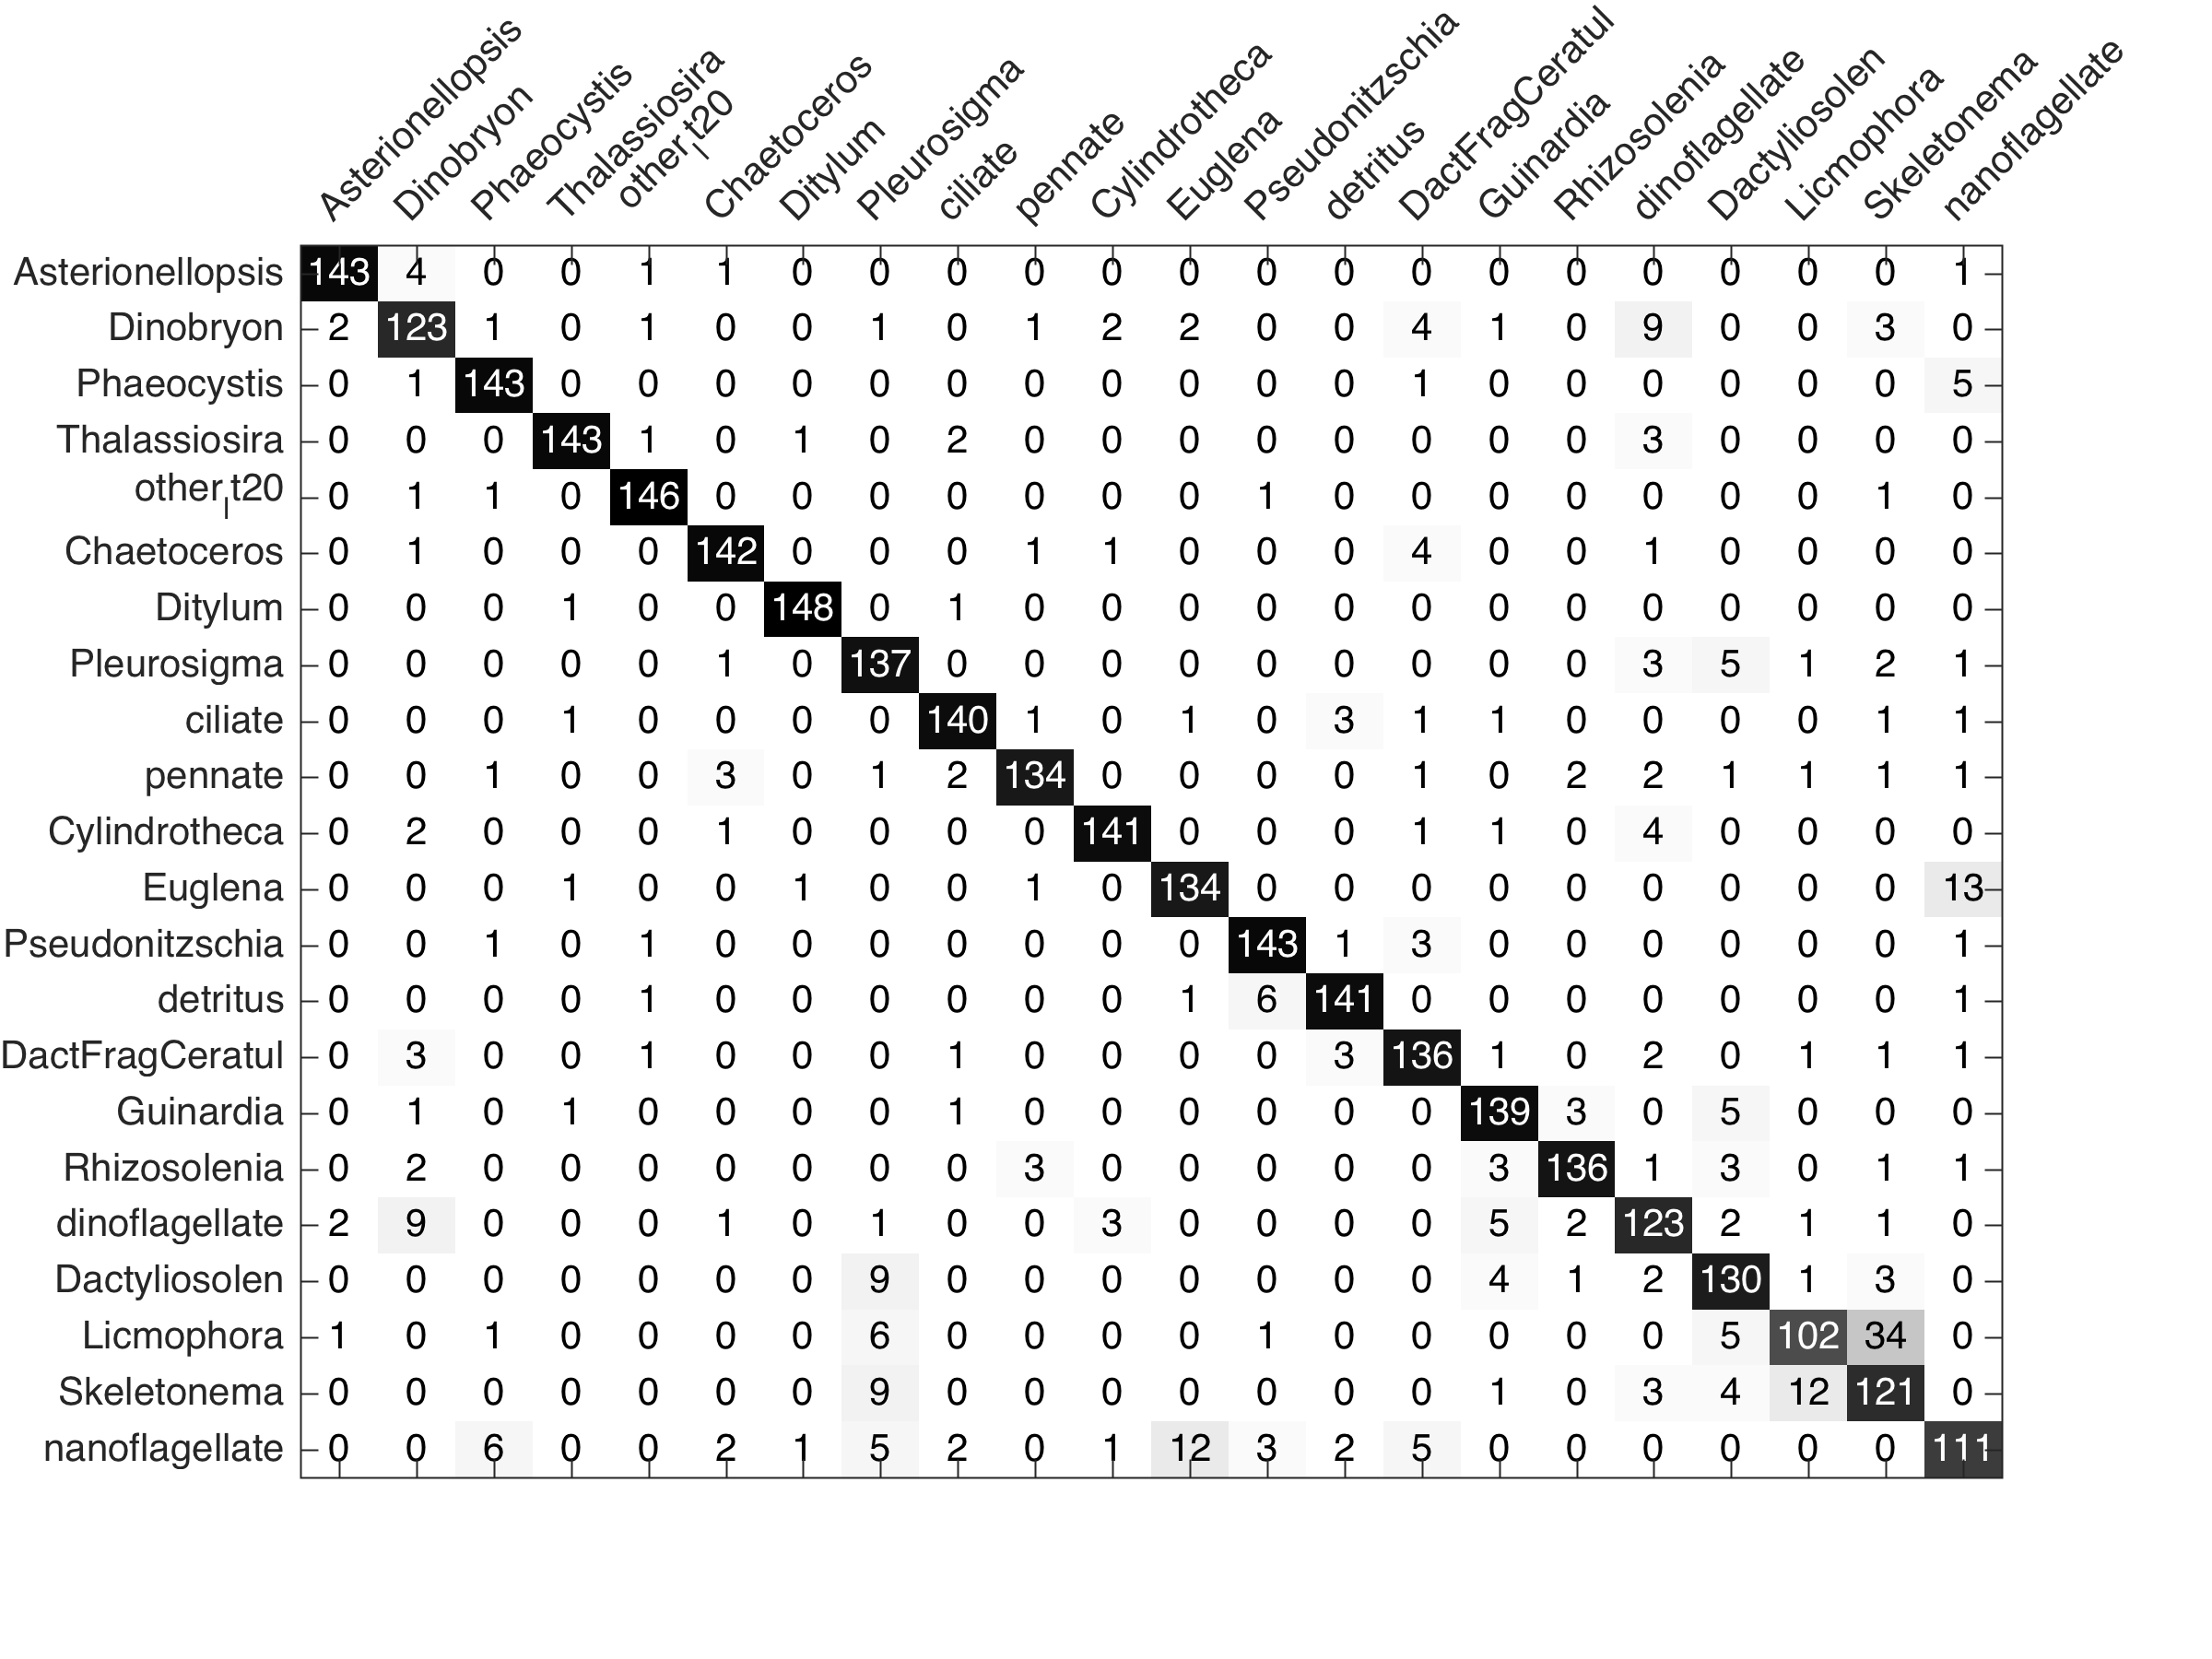
\includegraphics[height=5.3cm]{shiyan/shiyan2/whoiCM}}
  \subcaptionbox{ZooScan采集的数据集\label{fig:shiyan2zooscanCM}}
      {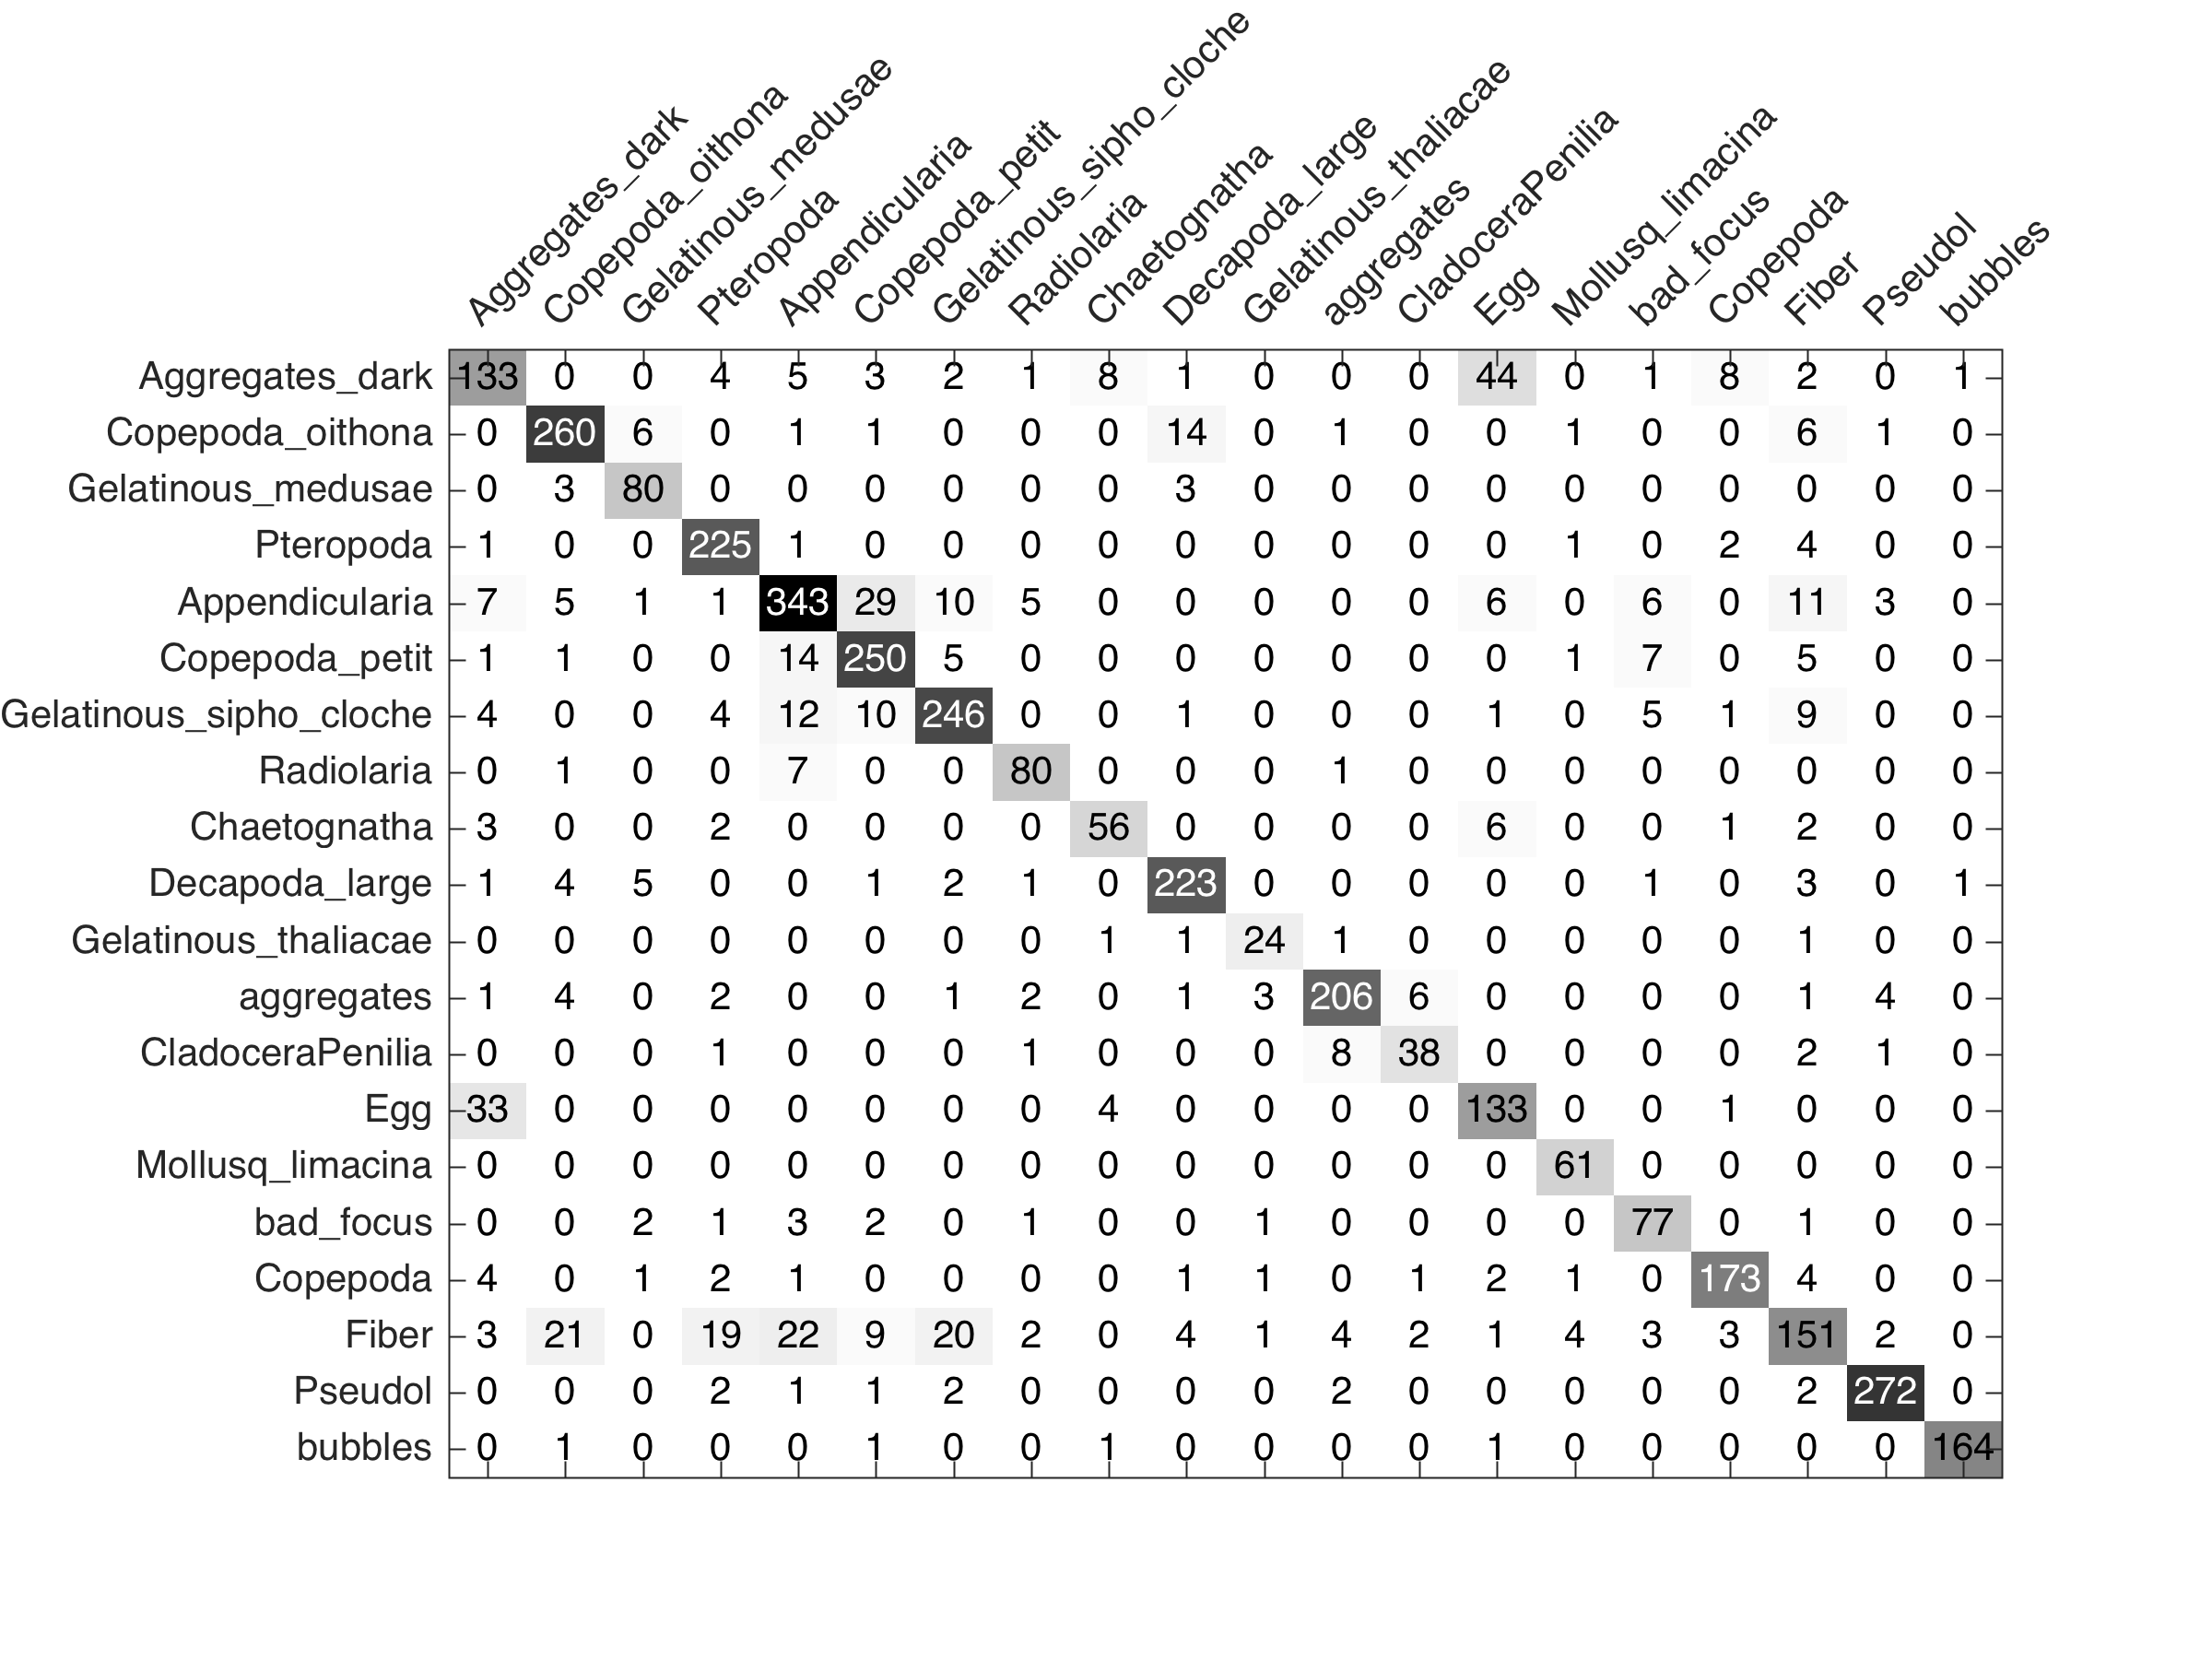
\includegraphics[height=5.8cm]{shiyan/shiyan2/zooscanCM}}\\
  ~\newline
  %\hspace{2em}%
  \subcaptionbox{Kaggle竞赛数据集\label{fig:shiyan2kaggleCM}}
      {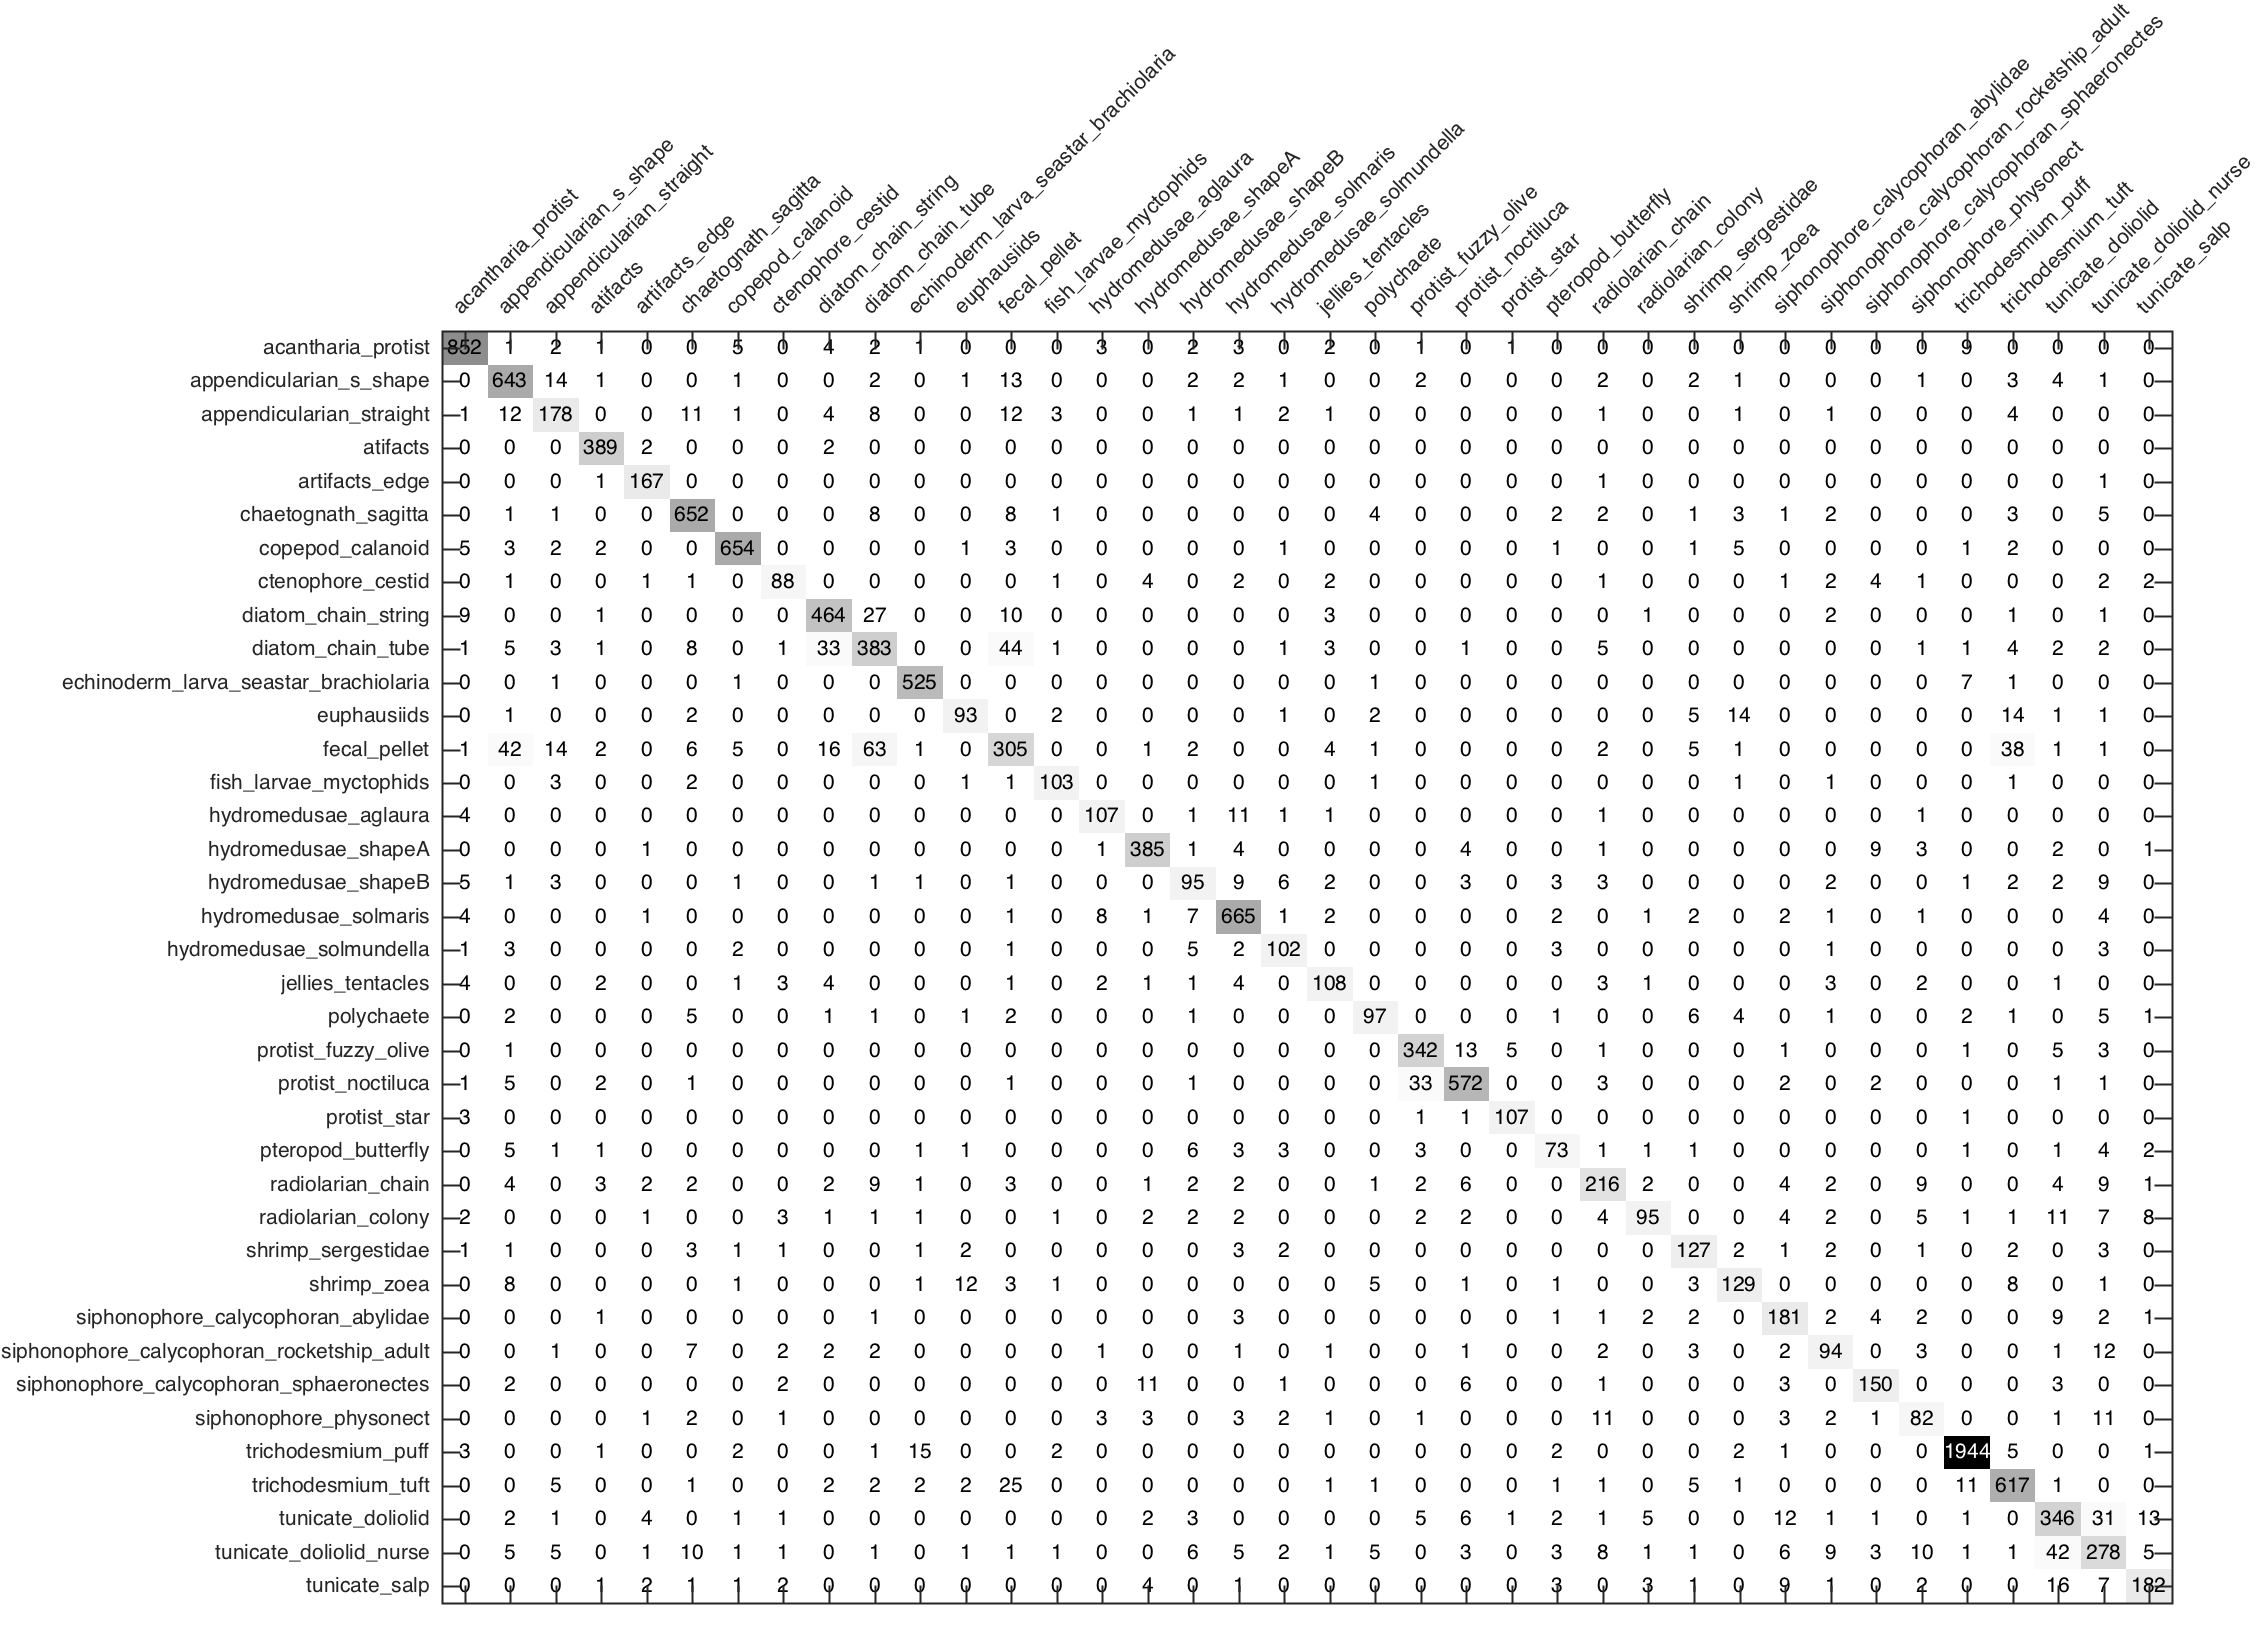
\includegraphics[height=11cm]{shiyan/shiyan2/kaggleCM}}
  \caption{特征对比实验最优分类结果的混淆矩阵}
  \label{fig:shiyan2}
\end{figure}

\subsection{基于多核学习的浮游生物图像分类实验}
\label{sec:ourExperiment}

将本文提出的基于多核学习的浮游生物分类系统分别在三个数据集上进行实验。在实验中为了对多核学习的性能进行分析,针对多核学习算法中的核函数种类设计了两组实验:(1)在多核学习时,每种特征只设定一种核函数,其算法流程如图~\ref{fig:shiyan31}所示,该组实验使用不同核函数和参数得到的分类结果如表~\ref{tab:shiyan31Result}所示;(2)每种特征使用三种核函数(分别为高斯核函数、多项式核函数、线性核函数),该实验的算法流程图如图~\ref{fig:shiyan32}所示,不同参数得到的分类结果如表~\ref{tab:shiyan32Result}。

\begin{figure}
\begin{minipage}{0.48\textwidth}
  \centering
  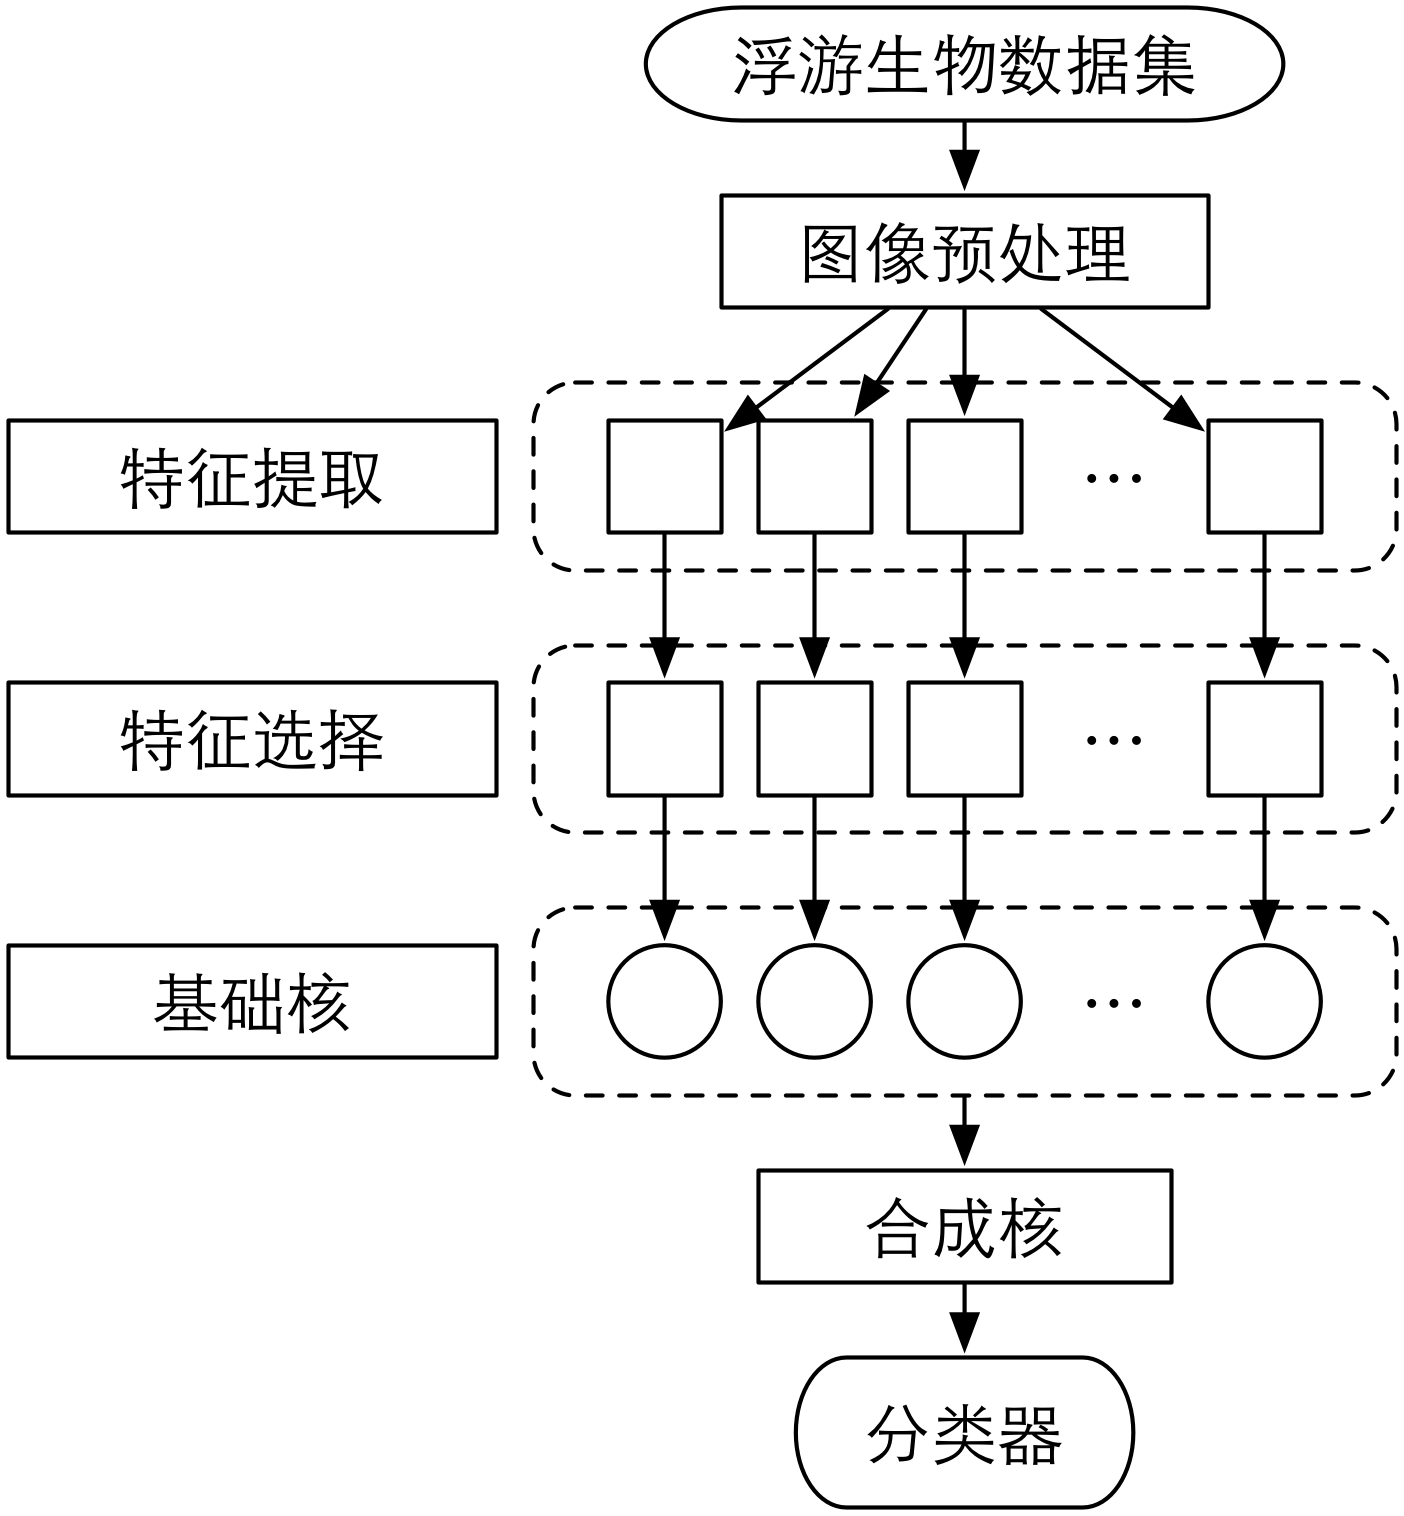
\includegraphics[height=6cm]{shiyan/shiyan3/shiyan31}
  \caption{基于多核学习的浮游生物分类的算法流程图(一种核函数)}
  \label{fig:shiyan31}
\end{minipage}\hfill
\begin{minipage}{0.48\textwidth}
  \centering
  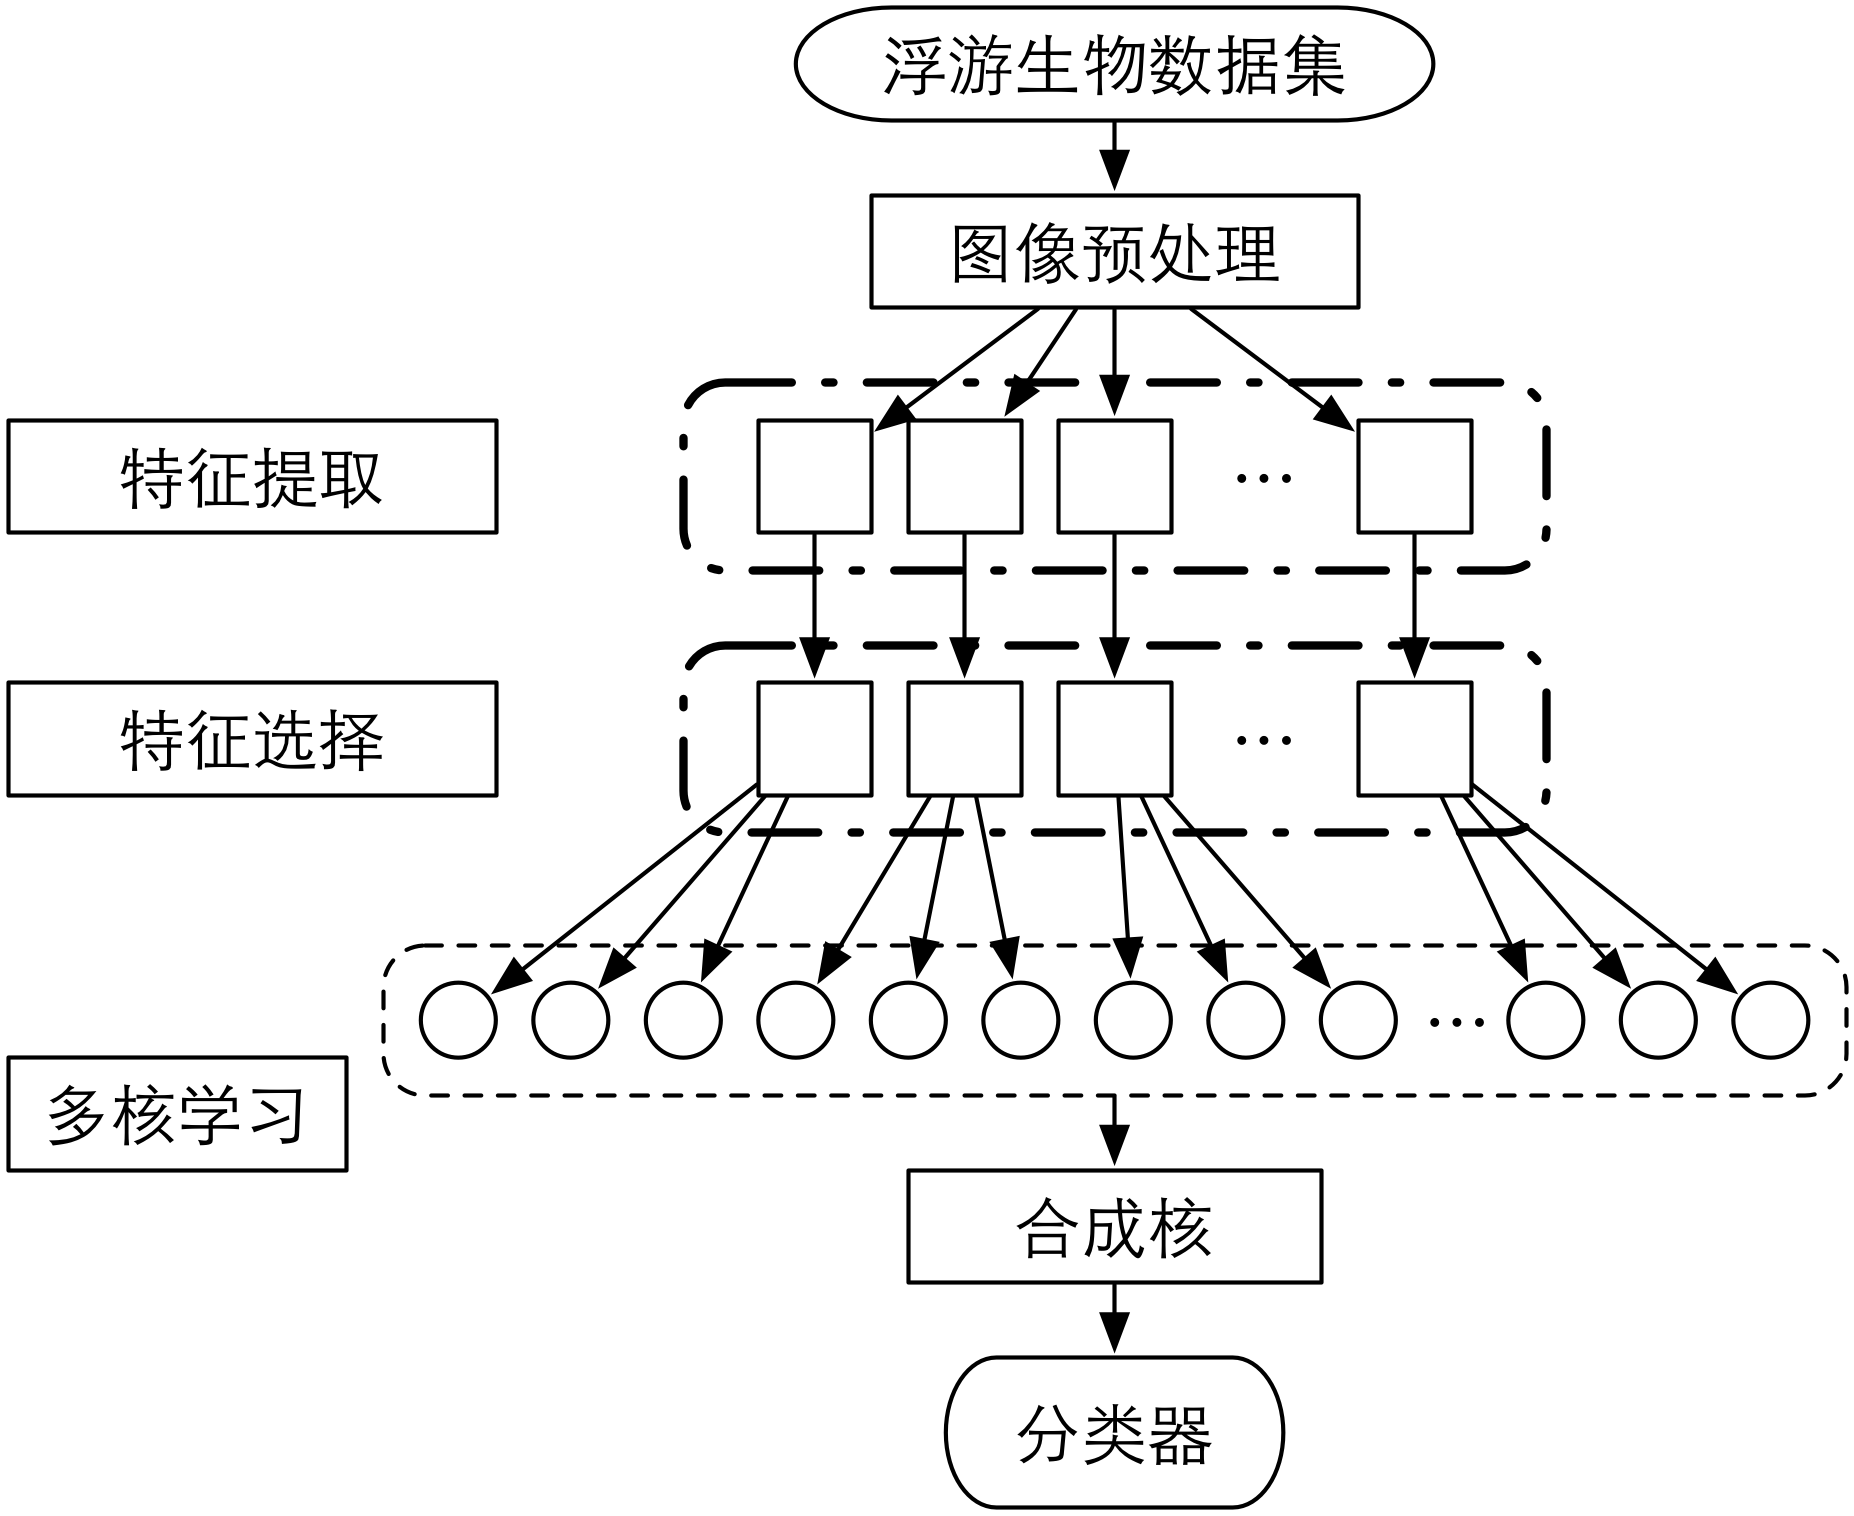
\includegraphics[height=6cm]{shiyan/shiyan3/shiyan32}
  \caption{基于多核学习的浮游生物分类的算法流程图(三种核函数)}
  \label{fig:shiyan32}
\end{minipage}
\end{figure}

\begin{table}[htbp]
\scriptsize
  \centering
  \caption{基于多核学习的浮游生物分类结果(一种核函数)}
  \label{tab:shiyan31Result}
  \begin{tabular}[c]{ccccccccccc}
    \toprule
    %\hline
    \multirow{2}*{数据集} & \multirow{2}*{C} & \multicolumn{3}{c}{高斯核函数} & \multicolumn{3}{c}{多项式核函数} & \multicolumn{3}{c}{线性核函数}\\
    %\cline{3-8}
     & & Recall & 1-Precision & F-Measure & Recall & 1-Precision & F-Measure & Recall & 1-Precision & F-Measure\\
    \midrule
    %\hline
    \multirow{3}*{WHOI数据集} & 1 & 0.8848 & 0.8865 & 0.8856 & 0.8958 & 0.8979 & 0.8968 & 0.8855 & 0.8882 & 0.8868\\
    %\cline{2-8}
     & 10 & 0.8875 & 0.8896 & 0.8885 & 0.8967 & 0.8984 & 0.8975 & 0.8912 & 0.8935 & 0.8923\\
    %\cline{2-8}
     & 100 & 0.8858 & 0.8880 & 0.8869 & 0.8939 & 0.8956 & 0.8947 & 0.8842 & 0.8859 & 0.8850\\
    \midrule
    %\hline
    \multirow{3}*{ZooScan数据集} & 1 & 0.8332 & 0.8826 & 0.8572 & 0.8394 & 0.8739 & 0.8553 & 0.8178 & 0.8447 & 0.8310\\
    %\cline{2-8}
     & 10 & 0.8626 & 0.8999 & 0.8809 & 0.8674 & 0.8824 & 0.8748 & 0.8398 & 0.8472 & 0.8435\\
    %\cline{2-8}
     & 100 & 0.8660 & 0.9008 & 0.8831 & 0.8679 & 0.8837 & 0.8757 & 0.8351 & 0.8437 & 0.8394\\
    \midrule
    %\hline
    \multirow{3}*{Kaggle数据集} & 1 & 0.7846 & 0.8259 & 0.8047 & 0.8039 & 0.8324 & 0.8179 & 0.7809 & 0.8076 & 0.7940\\
    %\cline{2-8}
     & 10 & 0.8295 & 0.8358 & 0.8326 & 0.8260 & 0.8438 & 0.8348 & 0.8132 & 0.8234 & 0.8183\\
    %\cline{2-8}
     & 100 & 0.8297 & 0.8316 & 0.8306 & 0.8211 & 0.8418 & 0.8313 & 0.7968 & 0.8090 & 0.8029\\
    \bottomrule
    %\hline
  \end{tabular}
\end{table}

\begin{table}[htbp]
\scriptsize
  \centering
  \caption{基于多核学习的浮游生物分类结果(三种核函数)}
  \label{tab:shiyan32Result}
  \begin{tabular}[c]{ccccc}
    \toprule
    %\hline
    \multirow{2}*{数据集} & \multirow{2}*{C} & \multicolumn{3}{c}{高斯核函数+多项式核函数+线性核函数}\\
    %\cline{3-4}
     & & Recall & 1-Precision & F-Measure\\
    \midrule
    %\hline
    \multirow{3}*{WHOI数据集} & 1 & 0.8964 & 0.8983 & 0.8973\\
    %\cline{2-4}
     & 10 & 0.8988 & 0.8997 & 0.8992\\
    %\cline{2-4}
     & 100 & 0.9000 & 0.9009 & 0.9004\\
    \midrule
    %\hline
    \multirow{3}*{ZooScan数据集} & 1 & 0.8542 & 0.8862 & 0.8699\\
    %\cline{2-4}
     & 10 & 0.8834 & 0.9042 & 0.8937\\
    %\cline{2-4}
     & 100 & 0.8831 & 0.9019 & 0.8924\\
    \midrule
    %\hline
    \multirow{3}*{Kaggle数据集} & 1 & 0.8030 & 0.8388 & 0.8205\\
    %\cline{2-4}
     & 10 & 0.8367 & 0.8551 & 0.8458\\
    %\cline{2-4}
     & 100 & 0.8346 & 0.8512 & 0.8428\\
    \bottomrule
    %\hline
  \end{tabular}
\end{table}

根据表~\ref{tab:shiyan31Result}能够发现,采用一种核函数在三个数据集上取得的最优分类结果为:在WHOI数据集上进行实验,采用多项式核函数且C = 10时得到的最优结果,F值为0.8975;在ZooScan采集的数据集上,采用高斯核函数且C=100时取得最优分类结果,F值为0.8831;在kaggle数据集上取得最优分类结果的F值为0.8348,对应的参数为多项式核函数且C=10。图~\ref{fig:shiyan3}为以上最优分类结果对应的混淆矩阵(图中横轴和纵轴为数据集中浮游生物的种类,见附录~\ref{fulu};图中数值表示分为对应类别图像的数量,数值越大颜色越深)。分析表~\ref{tab:shiyan32Result}可以得到使用三种核函数在三个数据集上的最优分类结果:WHOI数据集F值为0.9004;ZooScan数据集F值为0.8937;Kaggle数据集F值为0.8458。将本实验与之前的实验结果进行对比可以对基于多核学习的浮游生物分类系统的整体性能进行评价。
%Recall = 89.6\%, 1-Precision = 10.16\%;为Recall = 86.79\%, 1-Precision = 11.63\%;Recall = 82.6\%, 1-Precision = 15.62\%;
%Recall = 90\%,1-Precsion = 9.91\%;Recall = 88.34\%,1-Precision = 9.58\%;Recall = 83.67\%,1-Precision = 14.49\%

\begin{figure}[h]
  \centering%
  \subcaptionbox{WHOI采集的数据集\label{fig:shiyan3whoiCM}}%标题的长度,超过则会换行,如下一个小图。
    {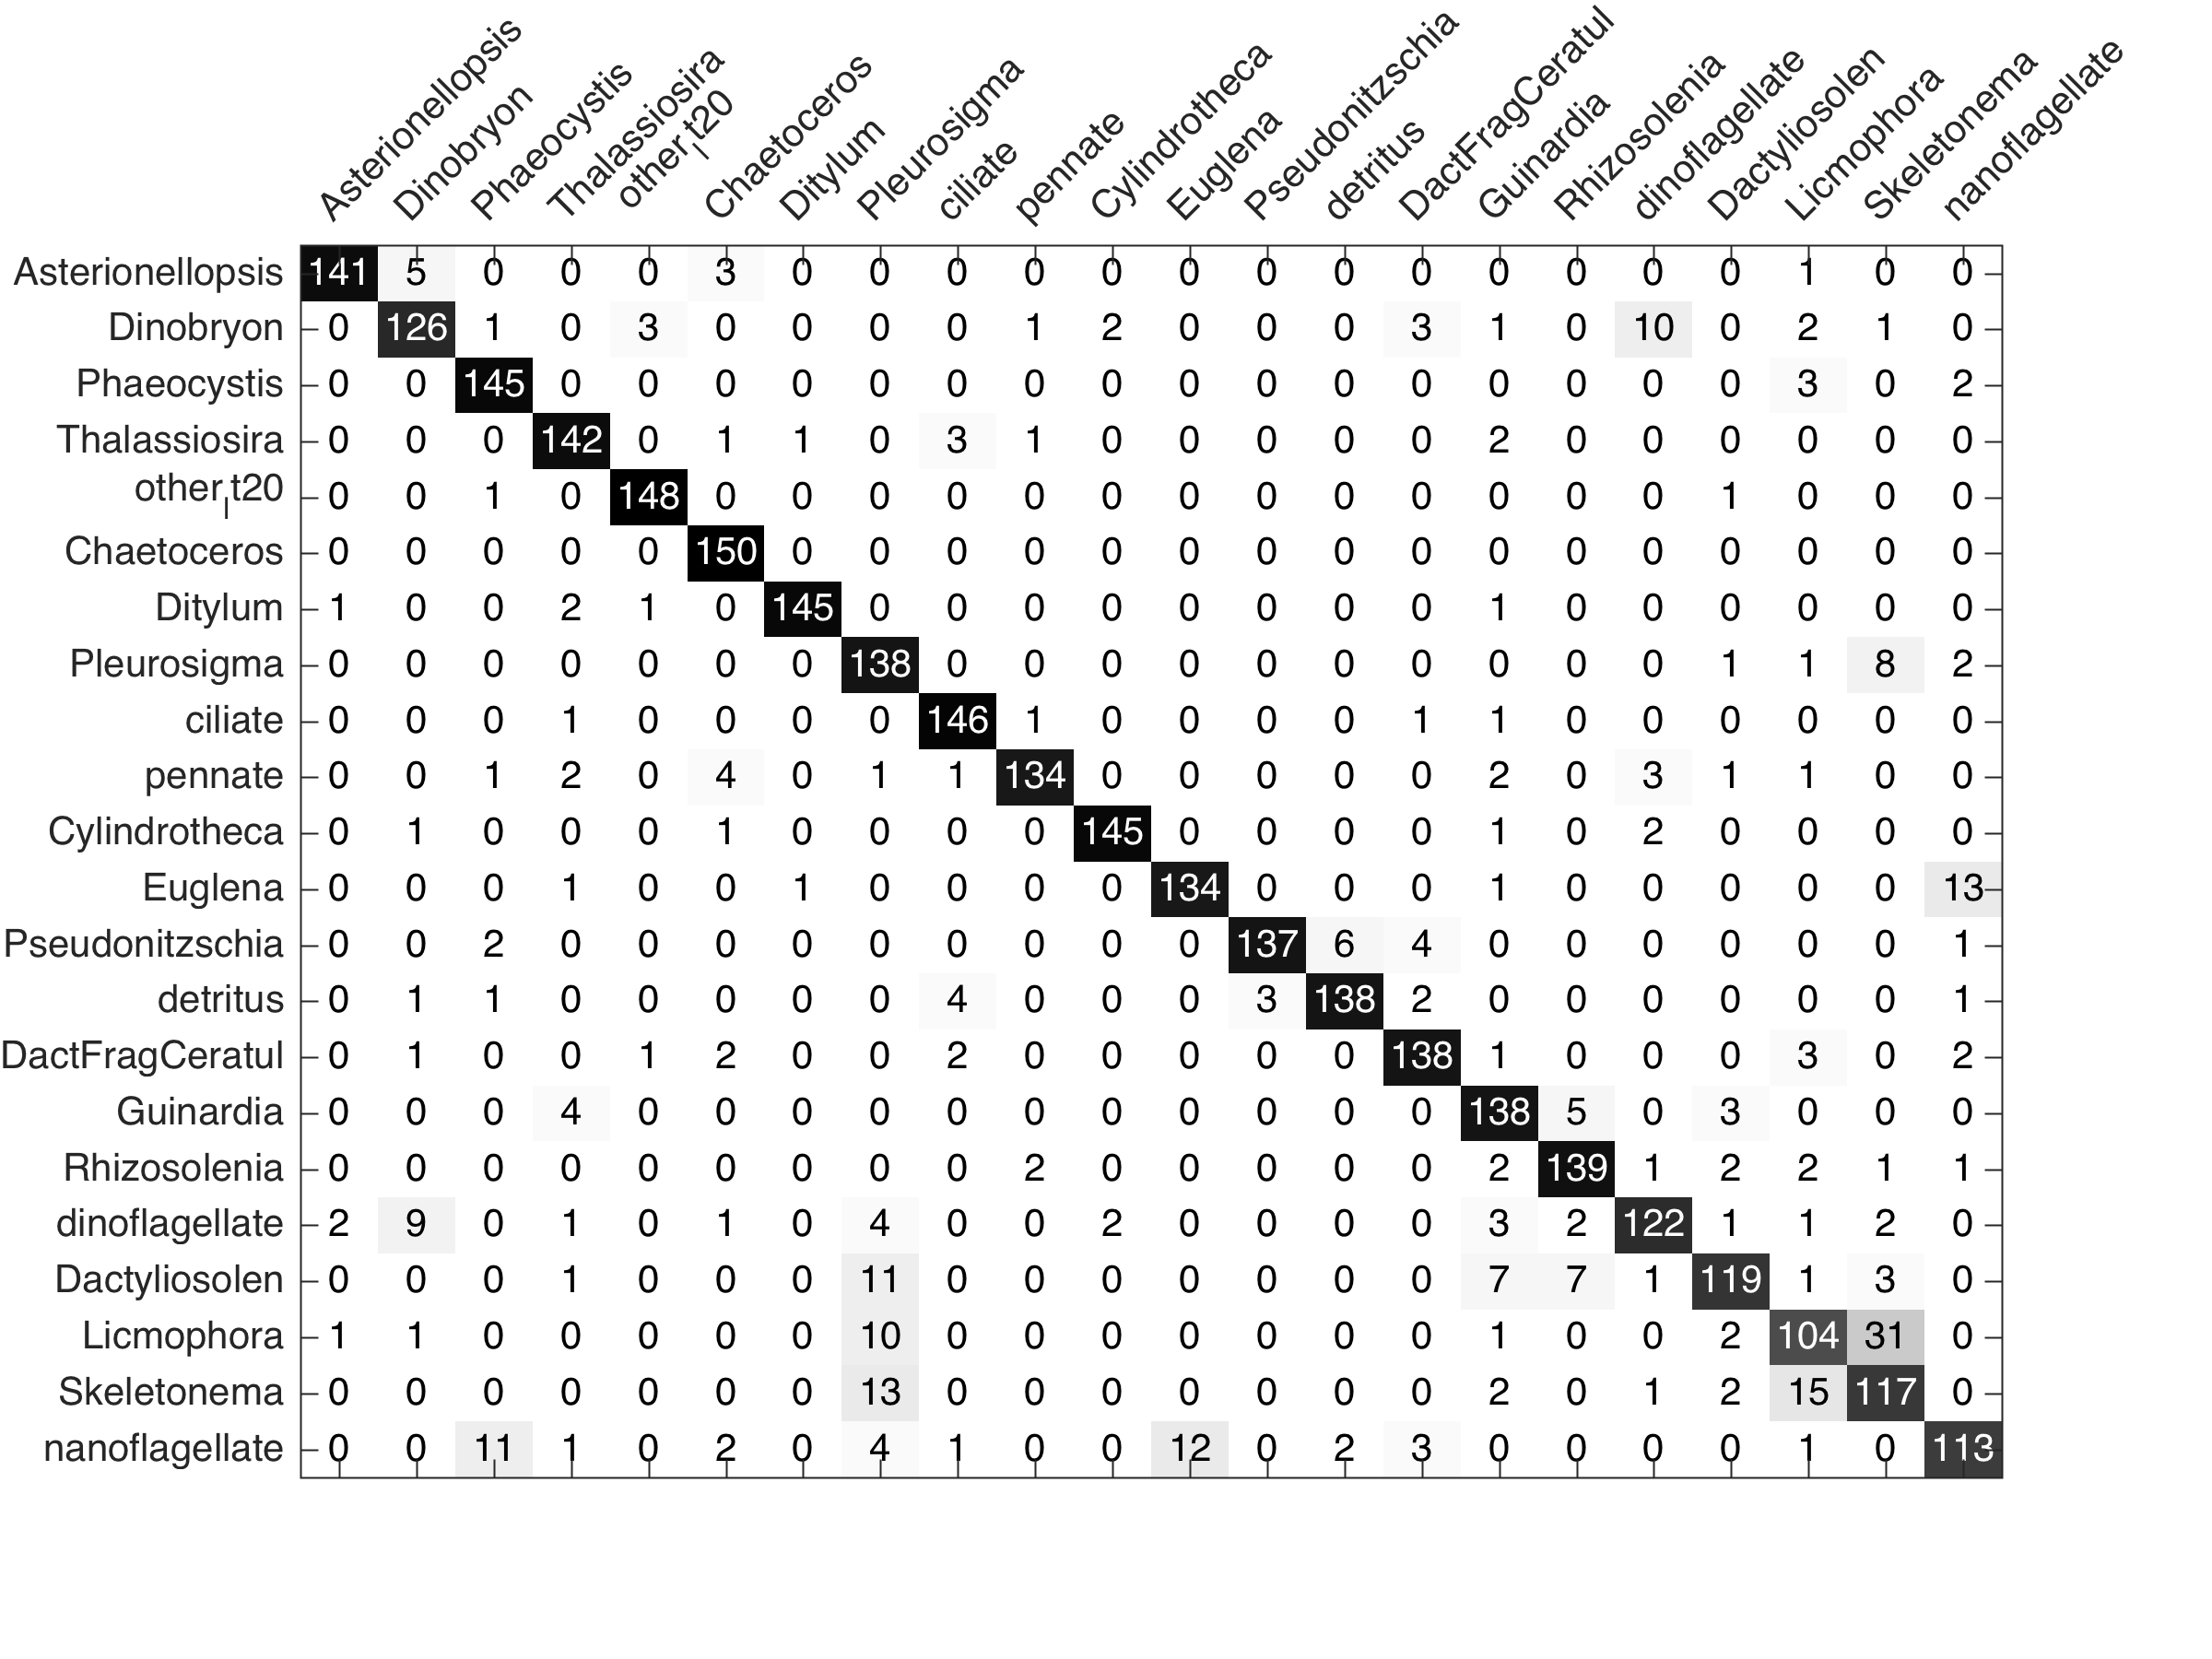
\includegraphics[height=5.5cm]{shiyan/shiyan3/whoiCM}}%\\%
  %~\newline
  %\hspace{2em}%
  \subcaptionbox{ZooScan采集的数据集\label{fig:shiyan3zooscanCM}}
      {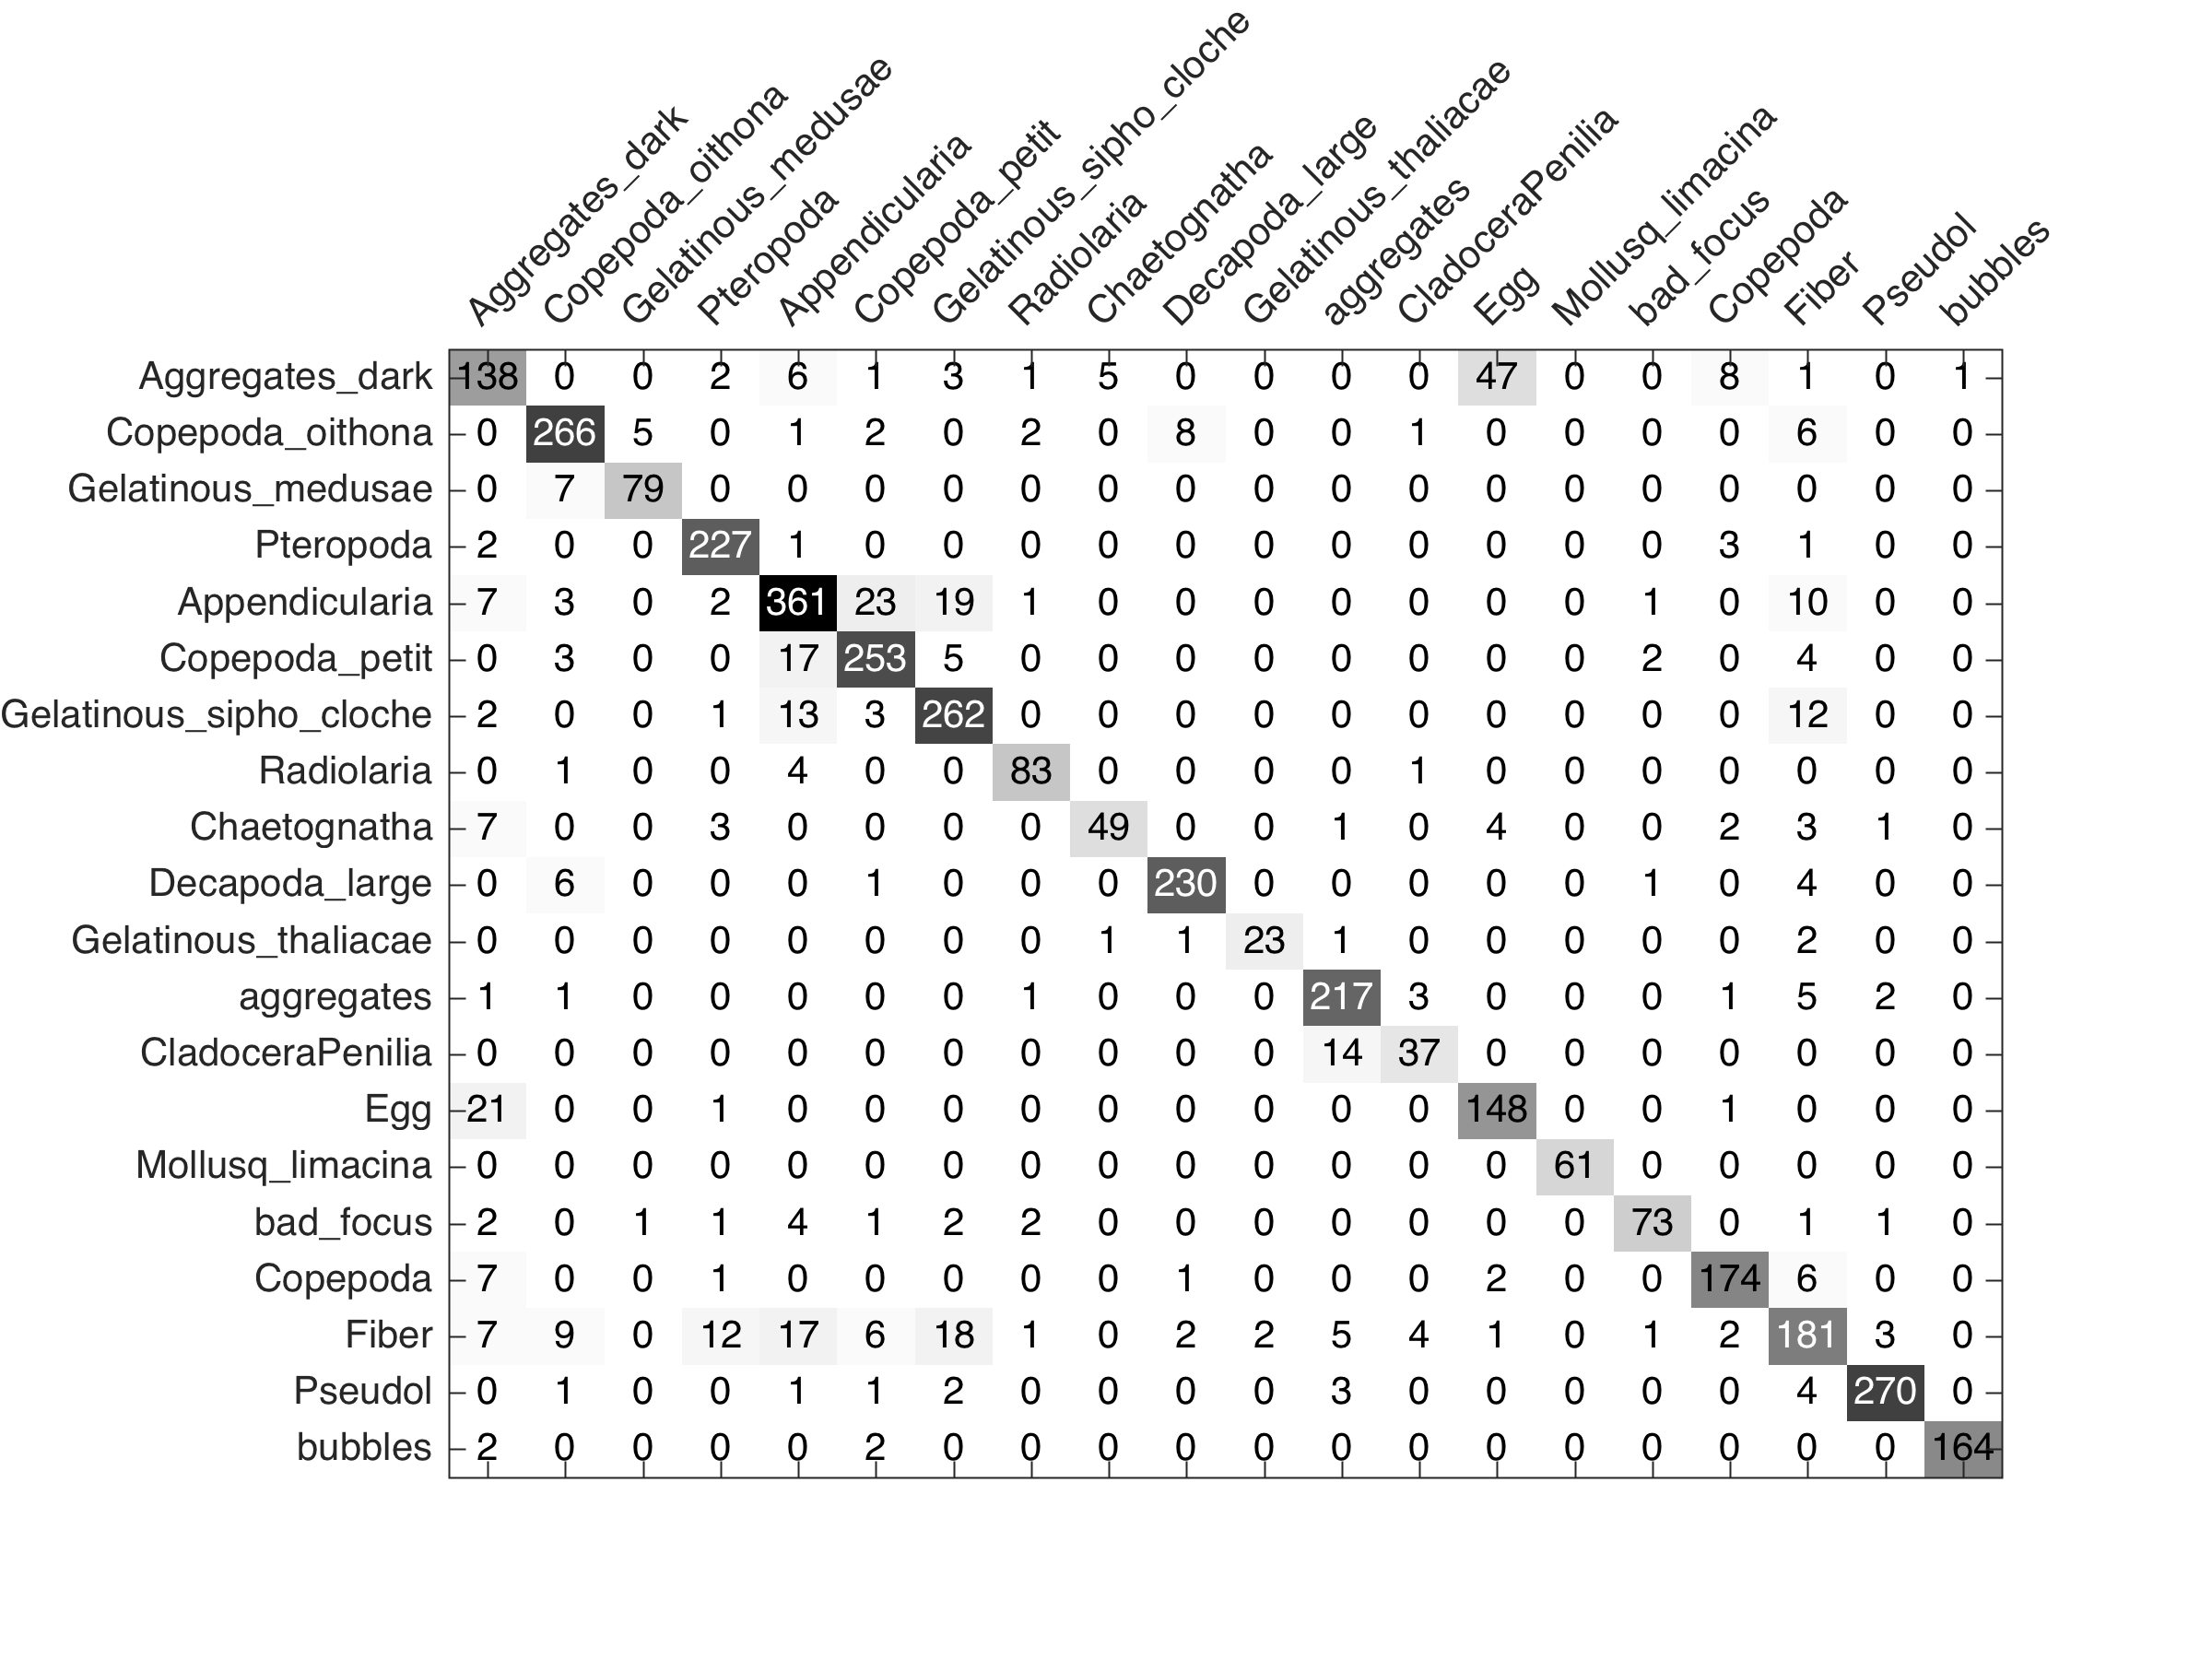
\includegraphics[height=6cm]{shiyan/shiyan3/zooscanCM}}\\
  ~\newline
  %\hspace{2em}%
  \subcaptionbox{Kaggle竞赛数据集\label{fig:shiyan3kaggleCM}}
      {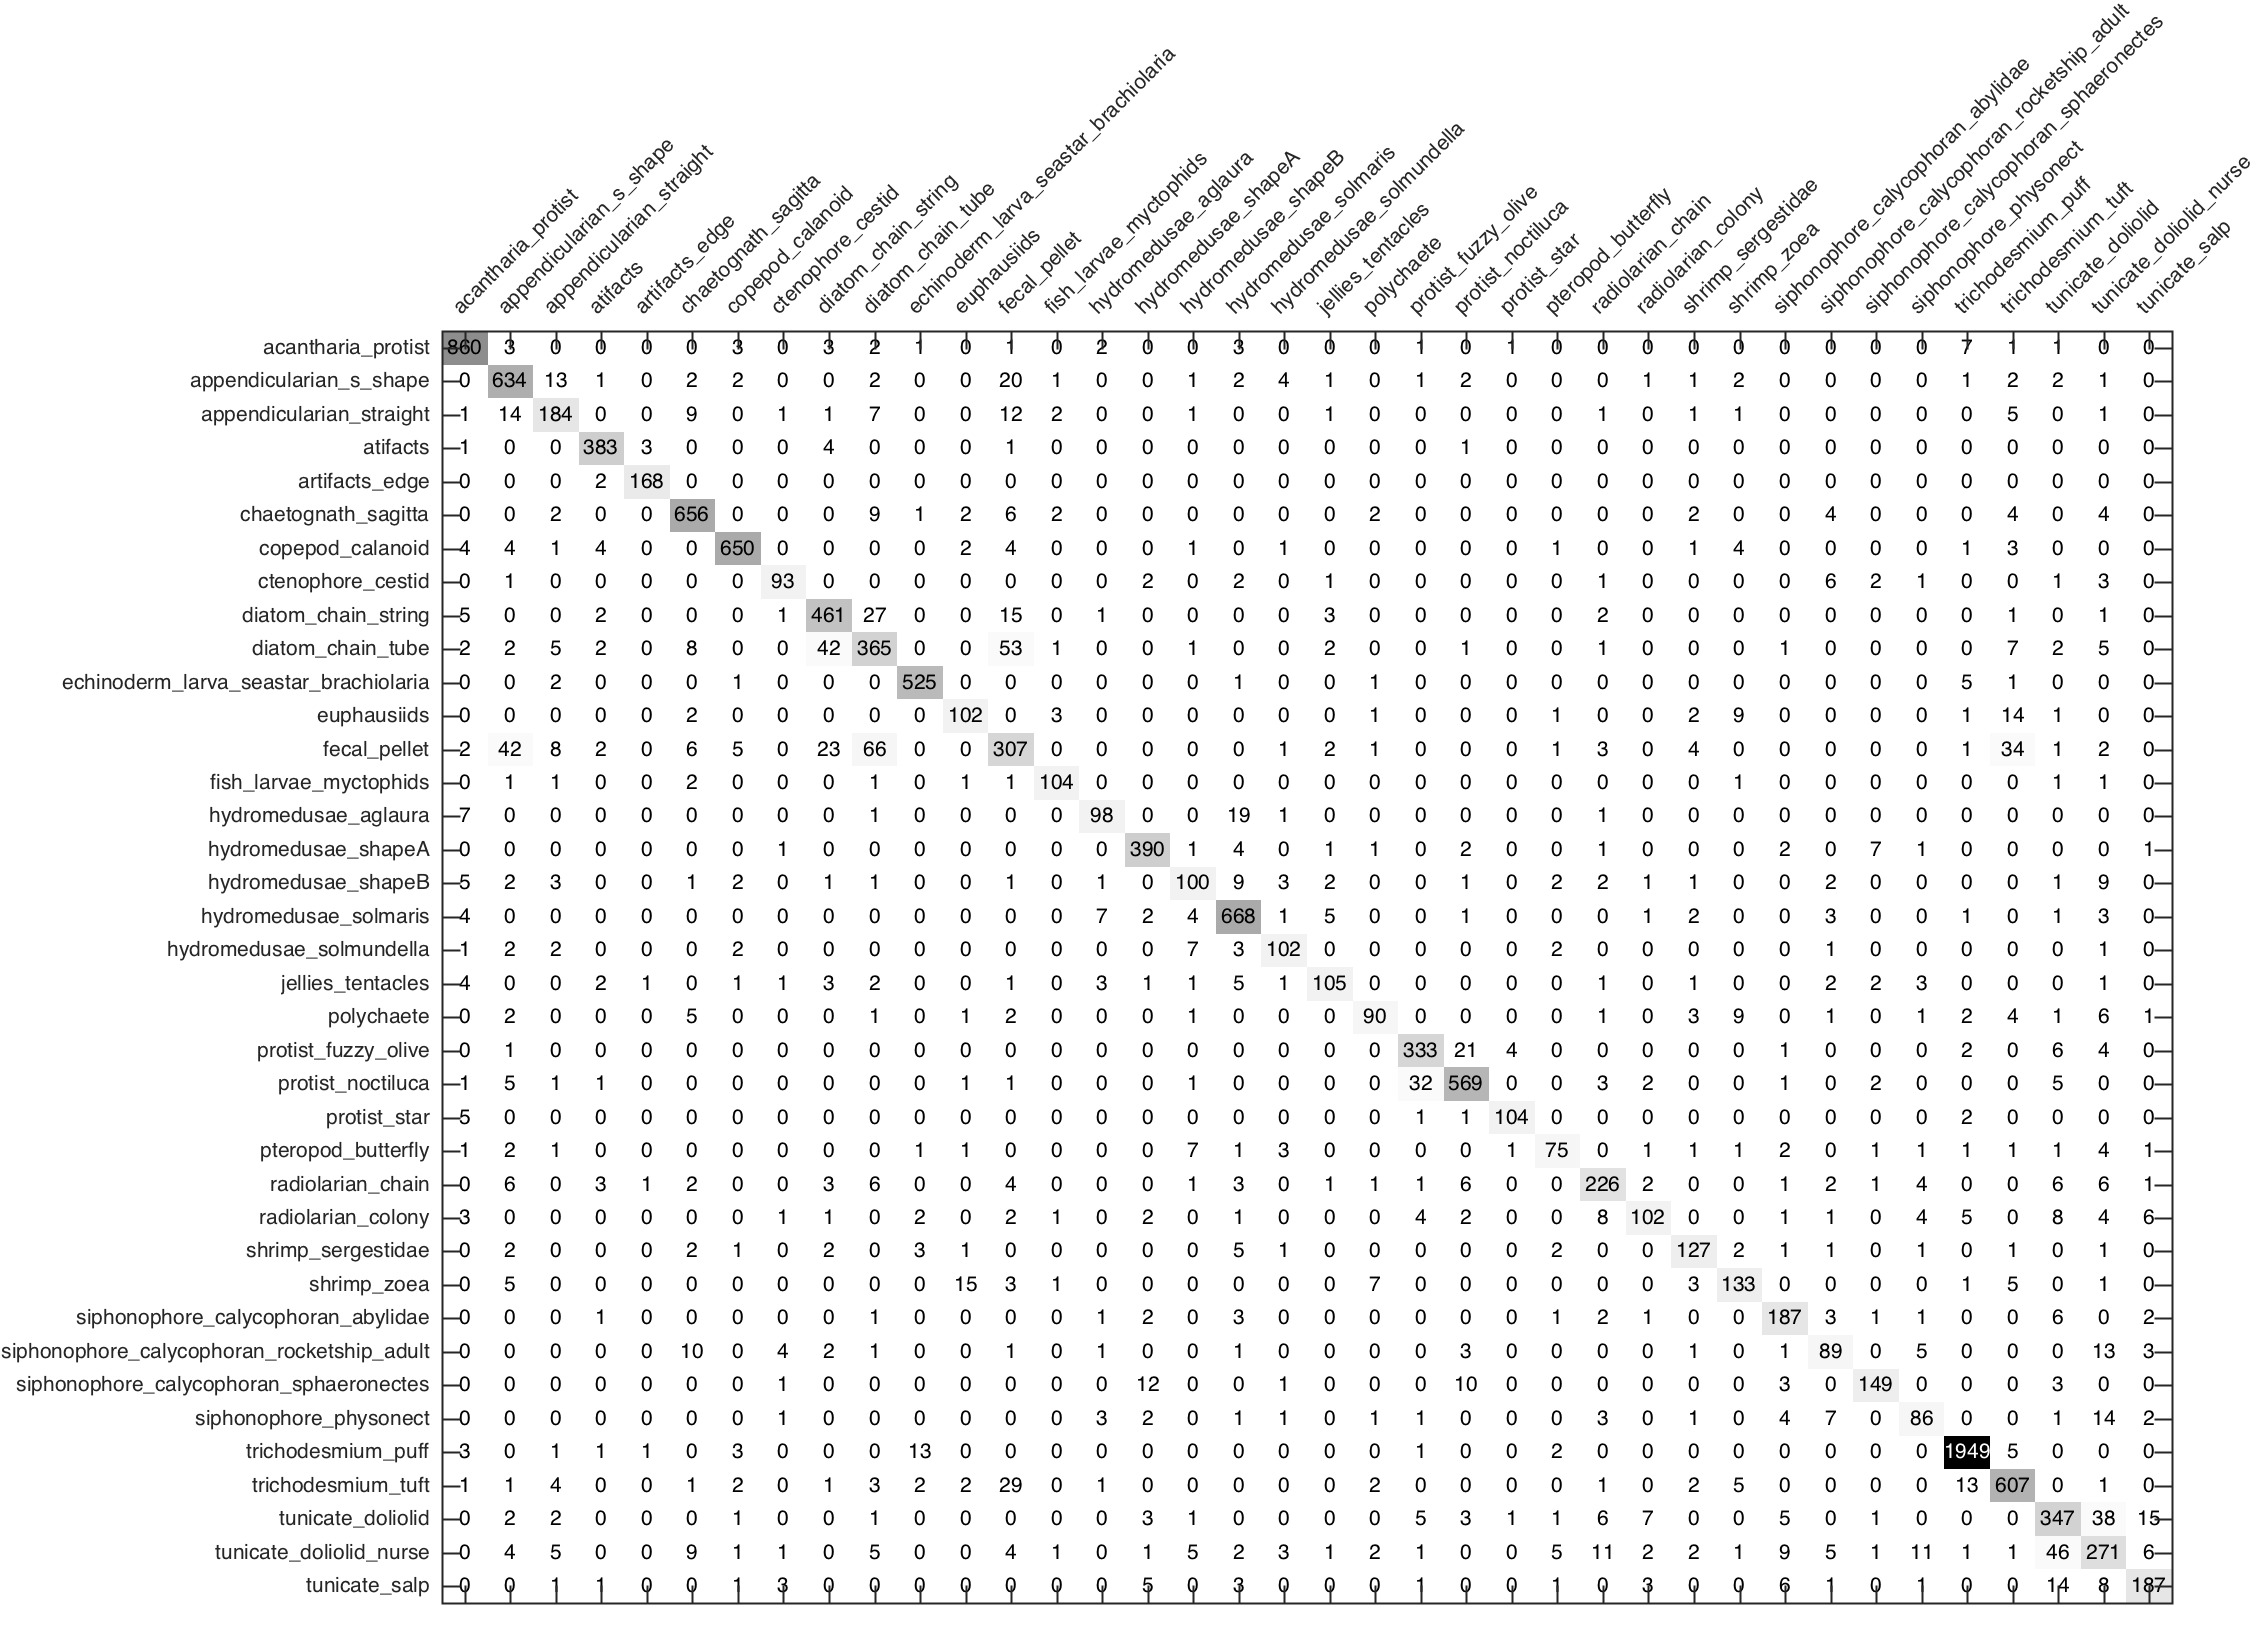
\includegraphics[height=11cm]{shiyan/shiyan3/kaggleCM}}
  \caption{基于多核学习的浮游生物最优分类结果的混淆矩阵(一种核函数)}
  \label{fig:shiyan3}
\end{figure}

\section{实验结果分析}

浮游生物包括浮游植物和动物两大类,这两类生物之间的形态差别较大。同时,浮游生物的种类繁多,按照“界门纲目科属种”的级别进行划分,从“界”到“种”,越向下被归为同一属的生物之间形态相差越小。以上这两个方面是浮游生物分类研究两个较大的难点。为了扩大浮游生物分类系统的适用范围,提高分类的准确率,我们提出了一种基于多核学习的浮游生物分类系统,该系统具有以下特点:首先,从多个角度对浮游生物的特征进行描述,具有较广的适用范围;其次,采用特征选择算法去除冗余特征;最后使用多核学习训练分类器,提高分类器的性能。

为了对本文提出的系统性能进行评价,在\ref{sec:experiment}中设计了三组对比实验。实验一为基准实验,综合目前性能较好的浮游生物分类方法设计而来,作为评价分类系统对比的基准。实验二是在实验一的基础上使用\ref{sec:FeatureExtraction}中的方法提取浮游生物特征,通过对比实验一与实验二的分类结果对特征提取方法的性能进行评价。实验三将本文设计的浮游生物分类系统在三个数据集上进行实验,将其分类结果与实验一和二对比来对分类系统总体性能进行评价。

根据表~\ref{tab:shiyan1Result}和表~\ref{tab:shiyan2Result},比较实验一与实验二在三个数据集上取得的最优分类结果可得表~\ref{tab:compare1and2}。从表~\ref{tab:compare1and2}中能够得出,实验二在三个数据集上取得的分类准确率比实验一都有一定程度的提高,同时错误率也相应的降低,其中在Kaggle数据集上的效果最为明显,F值提高了0.0641,分类性能有明显提高。此外,对比图~\ref{fig:shiyan1}和图~\ref{fig:shiyan2}可以看出:与实验一相比,实验二得到的分类结果,在Kaggle竞赛数据集上有36个类别的准确提高了,在WHOI和ZooScan采集的数据集上分别有14、16个类别提高。由此可以看出,结合多种特征对浮游生物的形态特征进行全面描述有利浮游生物的区分。例如,图~\ref{fig:shiyan1zooscanCM}中“Appendicularia”类图像中有58张图在实验一中被错误的分为“Gelatinous\_sipho\_cloche”类,而在实验二中,这个数字从58下降到了10。因此,在分类过程中从多个角度的对浮游生物的形态特征进行描述,可以提高分类系统的性能。

\begin{table}[htbp]
\small
  \centering
  \caption{特征对比实验与基准实验分类结果的对比}
  \label{tab:compare1and2}
  \begin{tabular}[c]{cc}
    \toprule
    %\hline
    数据集 & F-Measure提高量\\
    \midrule
    %\hline
    WHOI数据集 & 0.0131\\
    %\hline
    ZooScan数据集 & 0.0397\\
    %\hline
    Kaggle数据集 & 0.0641\\
    \bottomrule
    %\hline
  \end{tabular}
\end{table}

% \begin{table}[htbp]
%   \centering
%   \caption{实验二与实验一分类结果的对比}
%   \label{tab:compare1and2}
%   \begin{tabular}[c]{ccc}
%     \toprule
%     %\hline
%     数据集 & Recall & 1-Precision\\
%     \midrule
%     %\hline
%     WHOI数据集 & 1.3\% & -1.33\%\\
%     %\hline
%     ZooScan数据集 & 4.79\% & -3.1\%\\
%     %\hline
%     Kaggle数据集 & 7.05\% & -5.16\%\\
%     \bottomrule
%     %\hline
%   \end{tabular}
% \end{table}

实验三包含了两组实验:一个是在多核学习过程中每种特征只选用一种核函数;另一个是在多核学习时每种特征使用三种核函数。对比表~\ref{tab:shiyan31Result}和表~\ref{tab:shiyan2Result}中最优分类准确率可以的表~\ref{tab:compare31and2},这是实验三中每种特征使用一种核函数的多核学习与实验二的对比结果,可以得出使用多核学习能够提高分类器的性能。观察混淆矩阵图~\ref{fig:shiyan2}和图~\ref{fig:shiyan3}可以发现:采用多核学习得到的分类结果,在WHOI采集的数据集中有11类图像分类结果得到了提高,在Kaggle数据集上有21类,而在ZooScan数据集上所有类别的准确率都得到了提高。由此可见,采用多核学习的分类系统相较于采用单核学习方法的分类系统有较好的性能。同时,对比表~\ref{tab:shiyan31Result}和~\ref{tab:shiyan32Result}得到表~\ref{tab:compare3},可以发现使用多核学习时每种特征采用三种不同的核函数会使分类准确率有进一步的提高。

\begin{table}[htbp]
\small
  \centering
  \caption{基于多核学习的浮游生物分类实验(一种核函数)与特征对比实验分类结果对比}
  \label{tab:compare31and2}
  \begin{tabular}[c]{cc}
    \toprule
    %\hline
    数据集 & F-Measure提高量\\
    \midrule
    %\hline
    WHOI数据集 & 0.0012\\
    %\hline
    ZooScan数据集 & 0.0122\\
    %\hline
    Kaggle数据集 & 0.0044\\
    \bottomrule
    %\hline
  \end{tabular}
\end{table}

% \begin{table}[htbp]
%   \centering
%   \caption{每种特征使用一种核函数得到的分类结果与实验二分类结果的对比}
%   \label{tab:compare31and2}
%   \begin{tabular}[c]{ccc}
%     \toprule
%     %\hline
%     数据集 & Recall & 1-Precision\\
%     \midrule
%     %\hline
%     WHOI数据集 & 0.1\% & -0.14\%\\
%     %\hline
%     ZooScan数据集 & 1.4\% & -1.57\%\\
%     %\hline
%     Kaggle数据集 & 0.19\% & -0.71\%\\
%     \bottomrule
%     %\hline
%   \end{tabular}
% \end{table}

\begin{table}[htbp]
\small
  \centering
  \caption{每种特征使用三种核函数和一种核函数得到的分类结果对比}
  \label{tab:compare3}
  \begin{tabular}[c]{cc}
    \toprule
    %\hline
    数据集 & F-Measure提高量\\
    \midrule
    %\hline
    WHOI数据集 & 0.0029\\
    %\hline
    ZooScan数据集 & 0.0106\\
    %\hline
    Kaggle数据集 & 0.0110\\
    \bottomrule
    %\hline
  \end{tabular}
\end{table}

根据表~\ref{tab:shiyan32Result}可得,我们提出的基于多核学习的分类系统在三个数据集的上最优分类结果的F值可以达到0.9004、0.8937、0.8458,与实验一基准系统的最优分类结果对比有很大提高,如表~\ref{tab:compare3and1}。其中在Kaggle数据集上的性能提高最明显,F值提高了0.0768。有此可以看出,本文提出的基于多核学习的浮游生物分类系统有较好的分类性能和较高的泛化能力,可以广泛的应用于浮游生物研究。

\begin{table}[ht]
\small
  \centering
  \caption{基于多核学习的浮游生物分类实验(三种核函数)与基准实验分类结果对比}
  \label{tab:compare3and1}
  \begin{tabular}[c]{cc}
    \toprule
    %\hline
    数据集 & F-Measure提高量\\
    \midrule
    %\hline
    WHOI数据集 & 0.0172\\
    %\hline
    ZooScan数据集 & 0.0725\\
    %\hline
    Kaggle数据集 & 0.0768\\
    \bottomrule
    %\hline
  \end{tabular}
\end{table}

% \begin{table}[ht]
%   \centering
%   \caption{基于多核学习的浮游生物分类系统与基准系统的分类结果的对比}
%   \label{tab:compare3and1}
%   \begin{tabular}[c]{ccc}
%     \toprule
%     %\hline
%     数据集 & Recall & 1-Precision\\
%     \midrule
%     %\hline
%     WHOI数据集 & 1.73\% & -1.72\%\\
%     %\hline
%     ZooScan数据集 & 7.74\% & -6.72\%\\
%     %\hline
%     Kaggle数据集 & 8.31\% & -7\%\\
%     \bottomrule
%     %\hline
%   \end{tabular}
% \end{table}

\section{本章小结}

本文提出了基于多核学习的浮游生物分类系统,该系统主要采用多核学习融合多种特征进行分类识别,提高了分类系统的泛化能力和分类性能。本章介绍了多核学习的原理,采用非线性多核学习来进行特征融合和训练分类器。为了检验分类系统的分类性能,我们还设计了三组实验进行对比。首先根据Sosik等人提出的浮游植物分类系统~\cite{sosik2007automated}和ZooScan系统~\cite{gorsky2010digital}设计基准分类系统,以此作为后续实验对比的基准;其次还设计了特征对比实验,对分类系统中特征提取部分的性能进行评价;最后采用本文设计的浮游生物分类系统进实验,对该分类系统的性能进行评价分析。在设计对比实验的同时为了检验系统的泛化能力,将所有的实验都分别在三个不同的数据集上进行。

\chapter{总结与展望}

\section{总结}

浮游生物自动分类系统是浮游生物检测的重要部分,它通过图像处理和模式识别方法对采集的浮游生物图像进行自动分类来实现。浮游生物自动分类可以解决人工分类专业水平要求高、费时、费力等问题,提高分类的效率,对浮游生物监测具有重要的研究意义。在本文中,我们从提高浮游生物分类系统的准确率、适用范围等方面出发,以特征提取、多核学习等知识为基础研究基于多核学习的浮游生物分类,主要工作内容如下:
\begin{enumerate}
\item 构建不同的浮游生物数据集,提高分类系统的适用范围。为了验证本文设计的分类系统的泛化能力,我们从网上搜集了不同机构和图像采集设备采集的浮游生物图像,构建三个不同的数据集进行实验,即包含浮游植物数据集,也包含浮游动物数据集。
\item 分析浮游生物的形态特征,选取合适的特征提取方法进行特征描述。人们对浮游生物进行分类时会根据其形状、纹理、大小等特征综合考虑。因此本文在设计浮游生物分类系统时,以人的识别方式为基础,分别提取了浮游生物的以下几类特征:几何灰度特征、纹理特征(例如Gabor滤波器、局部二值模式等)、局部特征(例如形状上下文、尺度不变特征变换等)、粒子测度。从多个角度对浮游生物进行全面描述,提取丰富的浮游生物特征信息,为后续分类做准备。
\item 从提取的特征中为每个数据集选取最优的特征组合,除去其中的冗余部分。采集的丰富的浮游生物特征中会存在不相关或冗余部分,它们会影响分类器的性能。在特征提取后采用特征选择去除其中的冗余部分,减少特征的维数,提高分类的准确率和泛化能力。
\item 分析多核学习理论,选用适合的多核学习方法训练分类器。在本文的分类系统中采用非线性多核学习,针对每种特征选定适合的核函数参数,实现特征的融合并充分发挥每种特征的分类性能。
\item 设计对比实验,建立合理的评价体系,对本文提出的分类系统各部分的性能进行评价。首先根据目前性能较好的浮游生物分类方法设计一个基准分类系统,作为对比评价的基准;然后进行特征对比实验,对分类系统特征提取部分的性能进行评价;最后,用本文设计的浮游生物分类系统进行实验,与之前两个实验对比,对多核学习以及整个分类系统的性能进行评价。
\end{enumerate}

\section{展望}

本文提出的基于多核学习的浮游生物分类系统已经取得了较高的分类准确率,并且用于不同的浮游生物数据集时都有较好的性能,但是对浮游生物图像分类还有几个方面要进行深入研究:
\begin{enumerate}
\item 在多核学习中,每个核函数会对应生成一个核矩阵,核矩阵的数量越多计算量越大,在一定程度上会影响训练时间。因此多核学习相对于单核学习算法的计算速度较慢。如何提高多核学习的计算速度,使该系统可以更好的用于浮游生物实时监测是接下来需要研究的内容之一。
\item 从本文方法在三个数据集上的实验结果可以发现,虽然本文方法对不均衡的数据集(即数据集中每个类别图像数量不等)的分类准确率有一定的提升,然而其分类准确度还低于均衡数据集,因此下一步可以针对数据集不均衡问题进行深入研究。
\end{enumerate}
%\include{data/chap06}


%%% 其它部分
\backmatter

%% 本科生要这几个索引,研究生不要。选择性留下。
% 插图索引
% \listoffigures
% % 表格索引
% \listoftables
% % 公式索引
% \listofequations


%% 参考文献
% 注意:至少需要引用一篇参考文献,否则下面两行可能引起编译错误。
% 如果不需要参考文献,请将下面两行删除或注释掉。
\bibliographystyle{thuthesis}
\clearpage %目录中显示的页码正确
\phantomsection %目录中的链接能正确跳转
\addcontentsline{toc}{chapter}{参考文献} %目录中以章的名义添加条目
\bibliography{ref/refs}


%% 附录
\begin{appendix}
\chapter{浮游生物种类}
\label{fulu}

实验构建的三个数据集中浮游生物的分类:

\begin{table}[ht]
\small
  \centering
  \caption{WHOI采集的数据集}
  \begin{tabular}[c]{cc}
    \toprule
    \multicolumn{2}{c}{浮游生物种类}\\
    \midrule
    Asterionellopsis & Euglena\\
    Dinobryon & Pseudonitzschia\\
    Phaeocystis & Detritus\\
    Thalassiosira & DactFragCeratul\\
    Other\_20 & Guinardia\\
    Chaetoceros & Rhizosolenia\\
    Ditylum & Dinoflagellate\\
    Pleurosigma & Dactyliosolen\\
    Ciliate & Licmophora\\
    Pennate & Skeletonema\\
    Cylindrotheca & Nanoflagellate\\
    \bottomrule
  \end{tabular}
\end{table}

\begin{table}[ht]
\small
  \centering
  \caption{ZooScan系统采集的数据集}
  \begin{tabular}[c]{cc}
    \toprule
    \multicolumn{2}{c}{浮游生物种类}\\
    \midrule
    Aggregates\_dark & Gelatinous\_thaliacae\\
    Copepoda\_oithona & Aggregates\\
    Gelatinous\_medusae & CladoceraPenilia\\
    Pteropoda & Egg\\
    Appendicularia & Mollusq\_limacina\\
    Copepoda\_petit & Bad\_focus\\
    Gelatinous\_sipho\_cloche & Copepoda\\
    Radiolaria & Fiber\\
    Chaetognatha & Pseudol\\
    Decapoda\_large & Bunnles\\
    \bottomrule
  \end{tabular}
\end{table}

\begin{table}[ht]
\small
  \centering
  \caption{Kaggle竞赛数据集}
  \begin{tabular}[c]{cc}
    \toprule
    \multicolumn{2}{c}{浮游生物种类}\\
    \midrule
    acantharia\_protist & jellies\_tentacles\\
    appendicularian\_s\_shape & polychaete\\
    appendicularian\_straight & protist\_fuzzy\_olive\\
    artifacts & protist\_noctiluca\\
    artifacts\_edge & protist\_star\\
    chaetognath\_sagitta & pteropod\_butterfly\\
    copepod\_calanoid & radiolarian\_chain\\
    ctenophore\_cestid & shrimp\_sergestidae\\
    diatom\_chain\_string & shrimp\_zoea\\
    diatom\_chain\_tube & siphonophore\_calycophoran\_abylidae\\
    echinoderm\_larva\_seastar\_brachiolaria & siphonophore\_calycophoran\_rocketship\_adult\\
    euphausiids & siphonophore\_calycophoran\_sphaeronetes\\
    fecal\_pellet & siphonophore\_physonect\\
    fish\_larvae\_myctophids & trichodesmium\_puff\\
    hydromedusae\_aglaura & trichodesmium\_puff\\
    hydromedusae\_shapeA & trichodesmium\_tuft\\
    hydromedusae\_shapeB & tunicate\_doliolid\\
    hydromedusae\_solmaris & tunicate\_doliolid\_nurse\\
    hydromedusae\_solmundella & tunicate\_salp\\
    \bottomrule
  \end{tabular}
\end{table}

\end{appendix}

%% 致谢
% 如果使用声明扫描页,将可选参数指定为扫描后的 PDF 文件名,例如:
% \begin{acknowledgement}[scan-statement.pdf]
\begin{acknowledgement}
  
  转眼间三年的研究生生活即将结束,在这三年中我得到了导师、同门、家人以及朋友等许多人的帮助,在研究生生涯即将结束时,我想向这些给予我帮助的人们表示诚挚的感谢。

  首先,感谢导师姬光荣老师和郑海永老师对我的细心指导。在这三年的研究生生活中,郑老师教会我如何学习科研、如何工作思考、如何做人做事,他的严格要求让我养成好的习惯,并不断的提高自己。同时,我也十分感谢姬老师,在这三年里对我进行悉心指导,并给予我许多的关心和照顾。我研究生生活中最幸运的事就是可以同时有这两位老师的指导和关心,十分感谢两位老师为我所付出的一切。

  感谢朱亚菲师姐、孙晓庆师姐以及邱欣欣师姐,她们在科研和生活中给予我很大的帮助。感谢同级的伙伴们,你们的帮助陪伴伴随我走过了这美好难忘的三年。感谢实验室的师弟师妹们,这三年的时光因为你们而美好。

  感谢我的父母,你们对我的支持和无私付出,在我面对困难时给予我力量。在以后的日子里,我会更加努力,定不辜负你们的期望。

  感谢国家自然科学基金项目“基于视觉注意结合生物形态特征的海洋浮游植物显微图像分析”(批准号:61301240)、国家自然科学基金项目“基于生物形态特征的中国海常见有害赤潮藻显微图像识别”(批准号:61271406)、中央高校基本科研业务费项目“海洋浮游动物原位探测与分析系统”(批准号:201562023)的资助。

  最后,感谢所有关心和帮助过我的人,祝愿你们永远幸福快乐!
\end{acknowledgement}


%% 个人简历
\begin{resume}

  \resumeitem{个人简历}

  1992 年 5 月 14 日出生于 山东 省 威海 市。

  2010 年 9 月考入 浙江师范 大学 数理与信息工程 学院 电子信息工程 专业,2014 年 7 月本科毕业并获得 学士 学位。

  2014 年 9 月考入 中国海洋 大学 电子 系攻读 硕士 学位至今。

  \researchitem{发表的学术论文} % 发表的和录用的合在一起

  % 1. 已经刊载的学术论文(本人是第一作者,或者导师为第一作者本人是第二作者)
  \begin{publications}
    \item Wang R, Dai J, Zheng H, Ji G, Qiao X. Multi features combination for automated zooplankton classification, in Proceedings of OCEANS’16 MTS/IEEE Shanghai, 2016.
    \item Gu Z, Wang R, Dai J, Zheng H, Zheng B. Automatic searching of fish from underwater images via shape matching, in Proceedings of OCEANS’16 MTS/IEEE Shanghai. 2016.
  \end{publications}

  % 2. 尚未刊载,但已经接到正式录用函的学术论文(本人为第一作者,或者
  %    导师为第一作者本人是第二作者)。
  % \begin{publications}[before=\publicationskip,after=\publicationskip]
  %   \item Yang Y, Ren T L, Zhu Y P, et al. PMUTs for handwriting recognition. In
  %     press. (已被 Integrated Ferroelectrics 录用. SCI 源刊.)
  % \end{publications}

  % 3. 其他学术论文。可列出除上述两种情况以外的其他学术论文,但必须是
  %    已经刊载或者收到正式录用函的论文。
  % \begin{publications}
  %   \item Wu X M, Yang Y, Cai J, et al. Measurements of ferroelectric MEMS
  %     microphones. Integrated Ferroelectrics, 2005, 69:417-429. (SCI 收录, 检索号
  %     :896KM)
  %   \item 贾泽, 杨轶, 陈兢, 等. 用于压电和电容微麦克风的体硅腐蚀相关研究. 压电与声
  %     光, 2006, 28(1):117-119. (EI 收录, 检索号:06129773469)
  %   \item 伍晓明, 杨轶, 张宁欣, 等. 基于MEMS技术的集成铁电硅微麦克风. 中国集成电路,
  %     2003, 53:59-61.
  % \end{publications}

  \resumeitem{在学期间参加的研究项目} % 有就写,没有就删除
  \begin{enumerate}
  \item 国家自然科学基金项目“基于视觉注意结合生物形态特征的海洋浮游植物显微图像分析”(批准号:61301240)。
  \item 国家自然科学基金项目“基于生物形态特征的中国海常见有害赤潮藻显微图像识别”(批准号:61271406)。
  \item 中央高校基本科研业务费“海洋浮游动物原位探测与分析系统”(批准号:201562023)。
  \end{enumerate}

\end{resume}


%% 本科生进行格式审查是需要下面这个表格,答辩可能不需要。选择性留下。
% 综合论文训练记录表
%\includepdf[pages=-]{scan-record.pdf}
\end{document}
